\documentclass[
    11pt,
    a4paper,
    egregdoesnotlikesansseriftitles,
    toc=chapterentrywithdots,
    twoside,openright,
    titlepage,
    parskip=half,
    headings=normal,  % reduces heading size
    listof=totoc,
    bibliography=totoc,
    index=totoc,
    captions=tableheading,  % caption below table
    chapterprefix,
    listof=flat,
    final
]{scrbook}


% details about your thesis
\newcommand{\titel}{Analyse und Überarbeitung des Graphical User Interfaces von EB GUIDE Studio 6 zur Steigerung der Usability}
\newcommand{\artderarbeit}{Bachelorarbeit}  % {Bachelorarbeit,Masterarbeit}
\newcommand{\autor}{Sandra Schumann}
\newcommand{\studiengang}{Medieninformatik}  % {Informatik,Wirtschaftsinformatik,Medieninformatik}
\newcommand{\matrikelnr}{302\,0357}
\newcommand{\erstgutachter}{Prof.\,Dr.~Korbinian Riedhammer}
\newcommand{\zweitgutachter}{Prof.\,Dr.~Matthias\,Teßmann}
\newcommand{\logo}{figures/TH-Nuernberg-RGB.png}
\newcommand{\keywords}{hot, fuzz}
 

% custom head and foot
\usepackage[automark]{scrlayer-scrpage}
\pagestyle{scrheadings}
\ihead{\headmark}
\chead{}
\ohead{\pagemark}
\renewcommand*\chaptermarkformat{\chapappifchapterprefix{\ }% 
  \thechapter.\enskip}

\RedeclareSectionCommand[tocindent=0pt]{section}
\RedeclareSectionCommand[tocindent=0pt]{subsection}
%\RedeclareSectionCommand[tocnumwidth=70pt]{chapter}

\usepackage{scrhack}

% other packages
\usepackage[utf8]{inputenc}
\usepackage[T1]{fontenc}
\usepackage{lmodern,relsize,textcomp,csquotes}
\usepackage{amsmath,amsfonts}
\usepackage[english, ngerman]{babel}  % flip for German thesis
\usepackage[final]{graphicx}
\usepackage{setspace,geometry,xcolor}
\usepackage{makeidx}
\usepackage{paralist,ifthen,todonotes}
\usepackage{url}
\usepackage{pdfpages}
\usepackage{here}
\usepackage{subfig}

% table setup
\usepackage{longtable}
\usepackage{array}
\usepackage{ragged2e}
\usepackage{lscape}

% pdf hyperref
\usepackage[
    bookmarks=true,
    bookmarksopen=true,
    bookmarksnumbered=true,
    bookmarksopenlevel=1,
    pdftitle={\titel},
    pdfauthor={\autor},
    pdfcreator={\autor},
    pdfsubject={\titel},
    pdfkeywords={\keywords},
    pdfpagelabels=true,
    colorlinks=true,
    linkcolor=red,
    urlcolor=magenta,
    anchorcolor=black,
    citecolor=cyan,
    filecolor=magenta,
    menucolor=red,
    plainpages=false,
    hypertexnames=true,
    linktocpage=true,
]{hyperref}
\usepackage[ngerman]{cleveref}


% configure your listings style
\usepackage{listings}
\lstset{
	language=csh,
	tabsize=3,
	extendedchars=true,
	frame=single,
	showstringspaces=true,
	numbers=left,
	numberstyle=\small,
	breakautoindent=true
}
\renewcommand\lstlistingname{Auflistung}

% page setup
% \setlength{\topskip}{\ht\strutbox}
\geometry{paper=a4paper,left=2.5cm,top=3.0cm,bindingoffset=.8cm}
\onehalfspacing
\frenchspacing
\clubpenalty = 10000
\widowpenalty = 10000 
\displaywidowpenalty = 10000

% some commands
\newcommand{\ua}{\mbox{u.\,a.\ }}
\newcommand{\zB}{\mbox{z.\,B.\ }}
\newcommand{\dahe}{\mbox{d.\,h.,\ }}
\newcommand{\bzw}{\mbox{bzw.\ }}
\newcommand{\bzgl}{\mbox{bzgl.\ }}
\newcommand{\eg}{\mbox{e.\,g.\ }}
\newcommand{\ie}{\mbox{i.\,e.\ }}
\newcommand{\wrt}{\mbox{w.\,r.\,t.\ }}
\newcommand{\etal}{\mbox{\emph{et.\,al.\ }}}


% TODO remove if not needed...
\usepackage{blindtext}
\usepackage{longtable}


\begin{document}

\setcounter{secnumdepth}{3}  % numerate subsections
\setcounter{tocdepth}{2}  % ...but don't include them in toc

\frontmatter
\include{cover}\cleardoublepage

% download the following form and complete it (hit save in your editor)
% https://intern.ohmportal.de/fileadmin/Gelenkte_Doks/Abt/SZS/SB/SB_0050_FO_Pruefungsrechtliche_Erklaerung_und_Erklaerung_zur_Veroeffentlichung_der_Abschlussarbeit_public.pdf
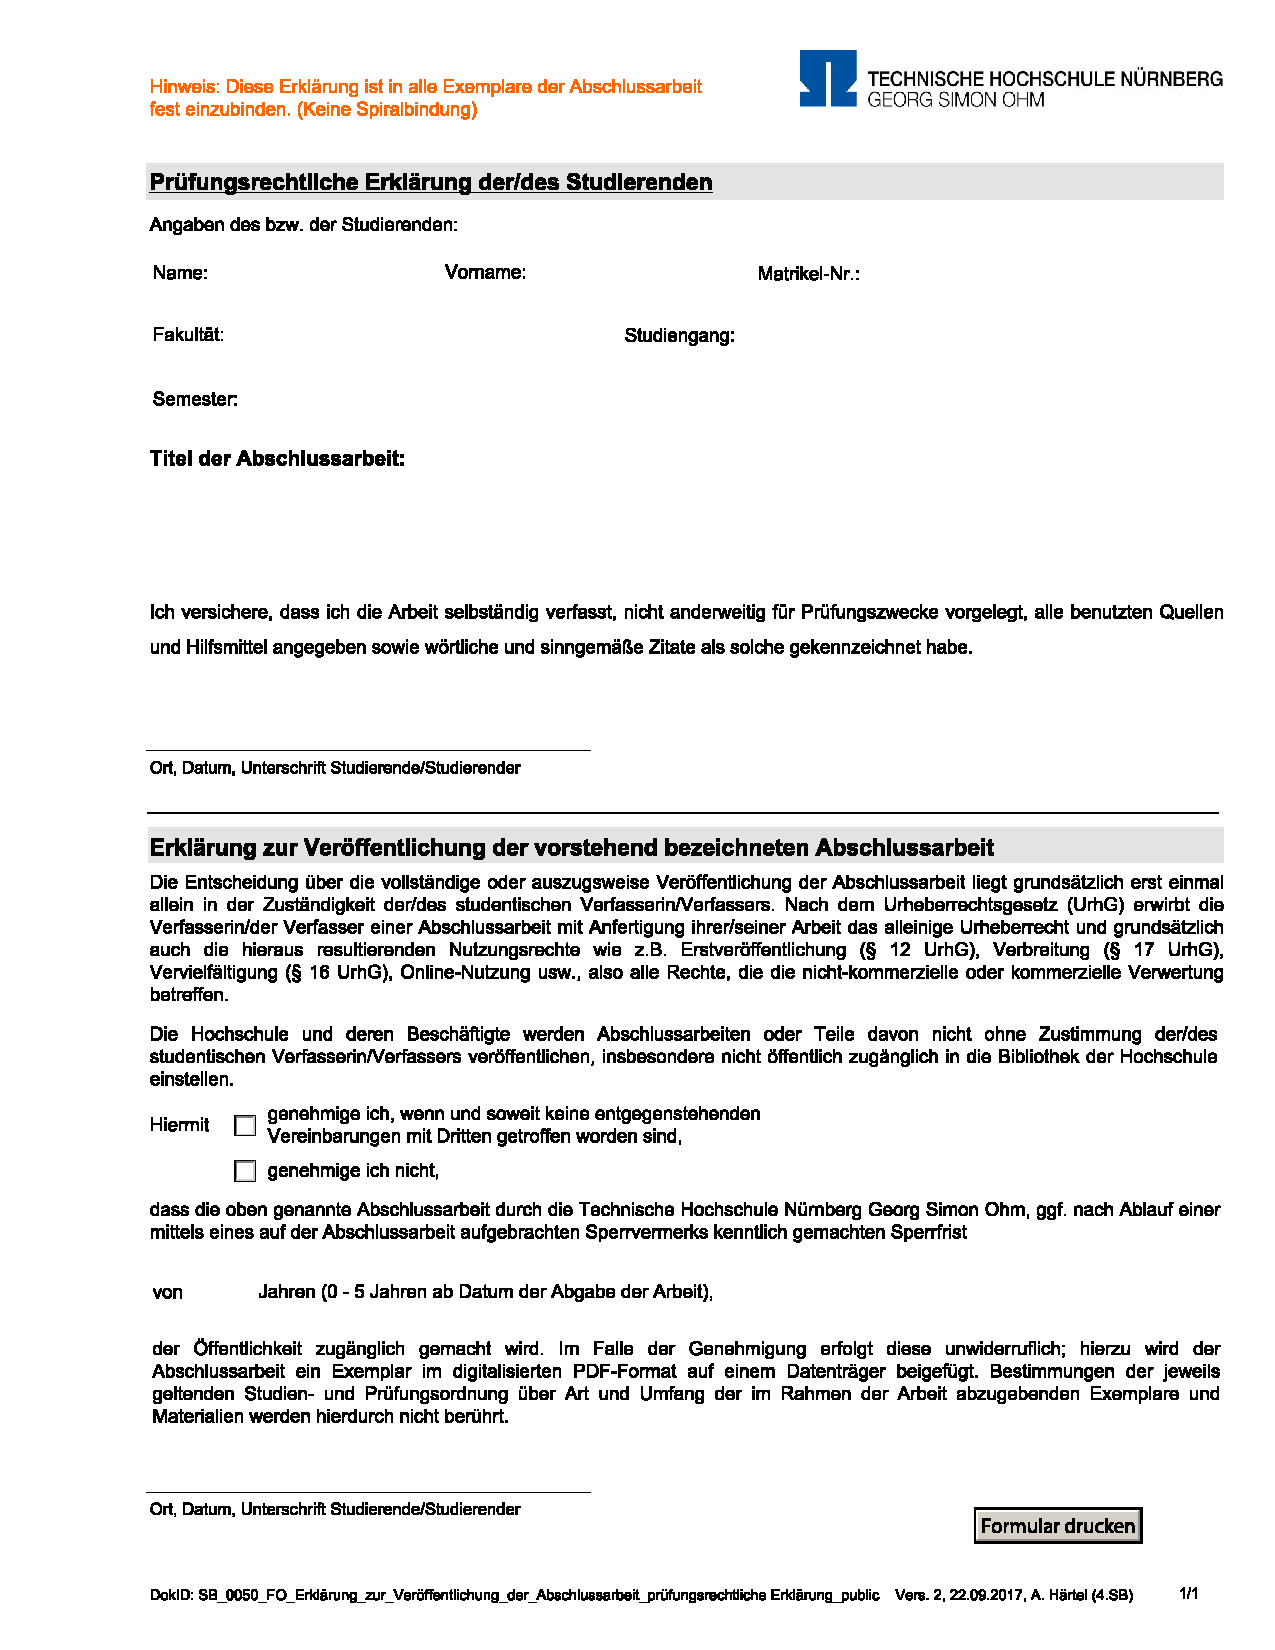
\includepdf{SB_0050_FO_Pruefungsrechtliche_Erklaerung_und_Erklaerung_zur_Veroeffentlichung_der_Abschlussarbeit_public.pdf}\cleardoublepage

\thispagestyle{empty}
\section*{Kurzdarstellung}
\label{sec:kurzdarstellung}

Die vorliegende wissenschaftliche Arbeit behandelt die Analyse und anschließende Überarbeitung des User Interfaces von EB GUIDE Studio 6, mit der Zielsetzung dessen Usability zu verbessern.
Um dies zu erreichen wurde sich an den einzelnen Iterationsschritten des Human-Centered Design Process orientiert.
Für die Identifizierung der Schwächen im Interface wurden Modellierer innerhalb der Zielgruppe bei ihrer täglichen Arbeit beobachtet und befragt.
Für drei dieser Schwächen wurden, nach allgemein gültigen Gestaltprinzipien, Verbesserungen erarbeitet, welche teilweise mithilfe eines Prototyping Tools und teilweise, im bestehenden Projekt, mit C\# und WPF umgesetzt wurden.
Die durchzuführende Testaufgabe wurde so ausgelegt, dass die Nutzer, während des Tests, mit allen eingearbeiteten Verbesserungen interagieren.
Um vergleichbare Werte zu erhalten wurde die Aufgabe von je fünf Nutzern mit dem bestehenden und dem überarbeiteten Interface durchgeführt.
Um die Usability zu messen wurde bei der Auswertung der Tests auf die Effizienz und Fehlerrate der Nutzer geachtet.

Nach einer Iteration des Design Process wird deutlich, dass die Anpassungen die Usability teilweise erhöht haben, die Verbesserungen jedoch auch noch Schwächen enthalten die Nachbesserung verlangen.
Hierfür können, aufbauend auf den durch diese Arbeit bereit stehenden Grundlagen, weitere Iterationen des Design Process durchgeführt werden, bis die Verbesserungen die Benutzeranforderungen hinreichend erfüllen.


\cleardoublepage

\tableofcontents

\mainmatter
\chapter{Einleitung}\label{ch:intro}

In diesem einführenden Kapitel wird zunächst kurz das Partnerunternehmen der Abschlussarbeit mit der zugehörigen Abteilung User Experience vorgestellt.
Weiterhin wird die Motivation dieser Arbeit und das verfolgte Ziel erläutert, bevor es noch einen Überblick über die folgenden Kapitel gibt.

\section{Elektrobit Automotive GmbH}
Partner der Bachelorarbeit ist die Firma Elektrobit Automotive GmbH - im Folgenden nur noch als EB bezeichnet.
EB ist ein vielfach ausgezeichnetes, internationales Unternehmen, welches sich auf die Entwicklung von Produkten und Dienstleistungen im Bereich der Automobilindustrie spezialisiert hat.
Mit über 30 Jahren Branchenerfahrung bietet EB seinen Kunden unter anderem innovative Lösungen für das vernetzte Fahrzeug, Human Machine Interface Technologien (HMI), Navigations- und Fahrassistenzsysteme und Steuergeräte. 
Die Automotive Software von EB befindet sich in über 1 Billionen Geräten, die in mehr als 90 Millionen Fahrzeugen weltweit Verwendung finden.
Mit über 2300 beschäftigten Mitarbeitern, verteilt auf 3 Kontinente und 9 Länder, und einer durchschnittlichen jährlichen Wachstumsrate von über 10 \%, ist EB ein weltweit etabliertes Unternehmen mit Hauptsitz in Erlangen\cite{about_eb}.

\section{Abteilung User Experience}
Jedes Gerät, das für den alltäglichen Gebrauch gedacht ist, sollte eine erfolgreiche Interaktion gewährleisten.
Dafür ist eine Schnittstelle zwischen Mensch und Maschine (HMI), die einen intuitiven, einfachen und schnellen Umgang mit diesem Gerät ermöglicht, unabdingbar.
Um die Erfahrungsqualität im Allgemeinen möglichst hoch zu halten, wünschen Nutzer sich auf ihre Bedürfnisse angepasste User-Interfaces in allen Lebensbereichen, womit der Bereich UX auch in der Automobilbranche einen hohen Bedeutungsgrad genießt.
Die Abteilung User Experience von EB befasst sich vor allem mit der Entwicklung multimodaler HMIs für Kombiinstrumente, Head Units und Head-Up Displays.
Diese werden von EB von der Konzeptphase bis hin zur Serienentwicklung mit Hilfe der Software EB-GUIDE entwickelt.

\section{Motivation}
Die in dieser Arbeit untersuchte Software, EB GUIDE, wird sowohl intern bei Elektrobit genutzt, als auch extern als Produkt vertrieben.
Bei firmeninterner Nutzung eines Produktes hängt die Usability des Selbigen direkt mit der Effektivität der damit durchgeführten Arbeit zusammen.
Dies begründet sich darin, dass Zeit, die Nutzer damit verbringen unklare Funktionen der Software zu verstehen, bezahlte Arbeitszeit darstellt ist der jedoch kein tatsächlicher Arbeitsfortschritt zu verzeichnen ist.
Darüber hinaus führt das fehlerhafte ausführen, oder nicht auffinden von Softwarefunktionen zu steigender Frustration des Nutzers, was ebenfalls die Produktivität negativ beeinflusst.

Für den Vertrieb einer Software ist schlechte Usability ebenfalls fatal.
Sobald es mehr als eine Software für ein Anwendungsgebiet gibt, werden Firmen die Software nutzen, die eine bessere Usability aufweist.
Diese Entscheidung begründet sich auf den gleichen Argumenten, weshalb Elektrobit bei  firmeninterner Nutzung eine Software mit hoher Usability bevorzugt.

Eine schlechte Usability von EB Guide hat also sowohl interne, als auch vertriebliche negative Folgen, weshalb Elektrobit es anstrebt die Usabiity der Software durchgehend zu verbessern.

\section{Zielsetzung}
Ziel dieser Bachelorarbeit ist es, Schwachstellen im User Interface von EB GUIDE zu identifizieren und durch deren Verbesserung die Usability von EB GUIDE zu erhöhen.
Dafür ist zuerst eine Analyse der Arbeitsabläufe innerhalb der Modellierungsarbeit nötig, um entsprechende Probleme im User Interface zu erkennen.
Anschließend gilt es, Konzepte zu entwickeln welche, durch Anpassung und Überarbeitung der entsprechenden Komponenten in der Benutzerschnittstelle, diese Probleme beheben oder minimieren.
Diese Konzepte werden anschließend noch grafisch und interaktiv visualisiert, um abschließende Usability-Tests durchführen zu können.
Dabei wird eine identische Aufgabenstellung von Probanden mit dem alten und dem überarbeiteten Interface durchgeführt und durch den Vergleich der Ergebnisse festgestellt, ob die Anpassungen die Usability von EB Guide erhöht haben.

\section{Aufbau der Arbeit}
Auf den folgenden Seiten werden zunächst die Theoretischen Grundlagen erläutert, die benötigt werden um eine Usabilitystudie durchzuführen und zu verstehen.
Dazu zählt auch das Prinzip des Human-Centered Design Process, nach dessen Iterationsschritten die Kapitel dieser Arbeit grob gegliedert sind.
Anschließend an die theoretischen Grundlagen werden Analysen an der bestehenden Software und am Arbeiterverhalten des Nutzer durchgeführt, um damit die existierenden Schwächen des Interfaces festzulegen und Verbesserungen erarbeiten zu können.
Diese werden im darauffolgenden Kapitel, in Form eines Prototyps umgesetzte oder direkt implementiert um die abschließenden Usability Tests durchführen zu können.
Abschließend werden die Ergebnisse dieser Tests ausgewertete und es wird ein kurzer Ausblick gegeben, welche Punkte in folgenden Iterationen des Design Process weiter verfolgt werden können.

\chapter{Theorie}\label{ch:data}

\section{Grafische Benutzeroberfläche}
Benutzerschnittstelle bezeichnet alle Komponenten eines interaktiven Systems, die dem Benutzer Interaktionsmöglichkeiten mit selbigem System bieten um ein verfolgtes Ziel zu erreichen.
Die grafische Benutzeroberfläche (GUI) bezeichnet hierbei den sichtbaren Anteil des Systems und damit nur einen Teil der gesamten Benutzerschnittstelle, zu der auch nicht sichtbare Teile wie z.B. die Funktionslogik beinhaltet sind.\cite{Sarodnick.2016}
Heutzutage sind die meisten Benutzeroberflächen auch grafische Benutzeroberflächen, mit denen in den häufigsten Fällen die Interaktion  über direkte Manipulation stattfindet.\cite{Nielsen.1995?}

\section{Ergonomie}
Unter Ergonomie versteht man im Allgemeinen die "Lehre von der menschlichen Arbeit und die Erkenntnis ihrer Gesetzmäßigkeiten"\cite{https:www.facebook.comArbeitsplatzergonomie.2014}.
Hierbei ist es wichtig zu verstehen, dass dabei der Fokus nicht ausschließlich auf einer technischen Komponente liegt, sondern das Zusammenspiel von Mensch, der zugeteilten Aufgabe und den verfügbaren Werkzeugen betrachtet wird\cite{Sarodnick.2016}.
Im Bezug auf Software bedeutet Ergonomie also konkret diese gut handhabbar und benutzerorientiert zu gestalten.

\section{Usability}
Mit immer höherer Komplexität von Systemen und Anwendungen kam der Begriff und das Verlangen nach  "Benutzerfreundlichkeit"\ auf.
Dieser Begriff suggeriert das lediglich die einfache Benutzung eines Systems ausschlaggebend ist, vernachlässigt hierbei jedoch die Notwendigkeit den Nutzer beim Erreichen seiner Ziele passend zu unterstützen.
Dies ist auch der Grund dafür das bald, statt auf "Benutzerfreundlichkeit"\ auf "Gebrauchstauglichkeit" (engl. Usability) geachtet wurde.
Im Gegensatz zur Ergonomie handelt es sich bei Usability nicht um eine eigenständige wissenschaftliche Disziplin, sondern um eine qualitative Anforderung an ein System\cite{Sarodnick.2016}.
Konkret spricht man bei einer Software-Anwendung von einer hohen Usability, wenn sie von der für sie bestimmten Zielgruppe effizient verwendet werden kann, also das verfolgte Ziel zufriedenstellend erreicht wird\cite{Richter.2016}.
Hierfür ist es entscheidend sich bewusst zu machen das ein technisches System oder Software immer Teil eines großen Handlungsablaufes ist und dazu dient Schritte dieses Handlungsablaufes zu erledigen.
Deshalb muss das System den Anforderungen dieses Ablaufes entsprechen und darf während der Entwicklung nicht getrennt davon betrachtet werden\cite{Sarodnick.2016}.

\section{User Experience}
Entgegen einer häufigen Annahme bezeichnen Usability und User Experience (UX) nicht das Gleiche.
Tatsächlich ist Usability lediglich ein Teil der gesamten User Experience eines Systems\cite{Knight.2019c}.
UX bezieht sich nicht nur auf die reine Nutzungszeit eines Systems, sondern berücksichtigt auch den Zeitraum davor und danach, bezeichnet als Antizipierte Nutzung und Verarbeitung der Nutzungssituation.
Usability ist hierbei, wie in \cref{fig:UX} zu sehen,  als wichtiger Faktor der User Experience in der aktiven Nutzungsphase zu betrachten, jedoch nicht mit dem Begriff gleichzusetzen \cite{Sarodnick.2016}.
Durch die zusätzliche Betrachtung der Effekte auf den Nutzer vor und nach der Nutzung, wie beispielsweise Erwartungen an das Produkt und Akzeptanz des selbigen, entstehen hier auch Verbindungen zur Gestaltung der Benutzerschnittstelle und dem Produkt-Design\cite{Richter.2016}.
Zusammenfassend lässt sich festhalten das Usability zwar die funktionsbezogene Betrachtungsweise abdeckt, die User Experience als ganzes jedoch auch emotionale Faktoren bezüglich Design und Ästhetik berücksichtigt um das Nutzungsvergnügen möglichst hoch zu halten.
Zusätzlich ist eine gute User Experience notwendig wenn ein Produkt auf dem Markt bestehen will.
Sobald es mehr als ein Produkt zur Lösung der gleichen Aufgabenstellung gibt, wird das mit der besseren User Experience Verwendung finden\cite{Knight.2019c}.

\begin{figure} [!h]
\begin{center}
  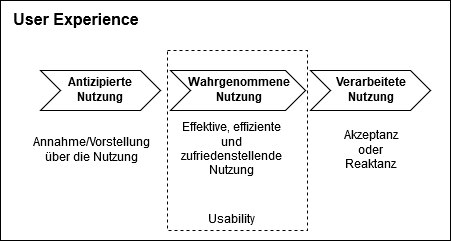
\includegraphics[scale=0.7]{figures/UX.png}
  \caption{Zusammenhang Usability und User Experience (nach \cite{Sarodnick.2016})}
  \label{fig:UX}
\end{center}
\end{figure}

\section{Human - Centered - Design - Process}
TODO

\begin{figure} [!h]
\begin{center}
  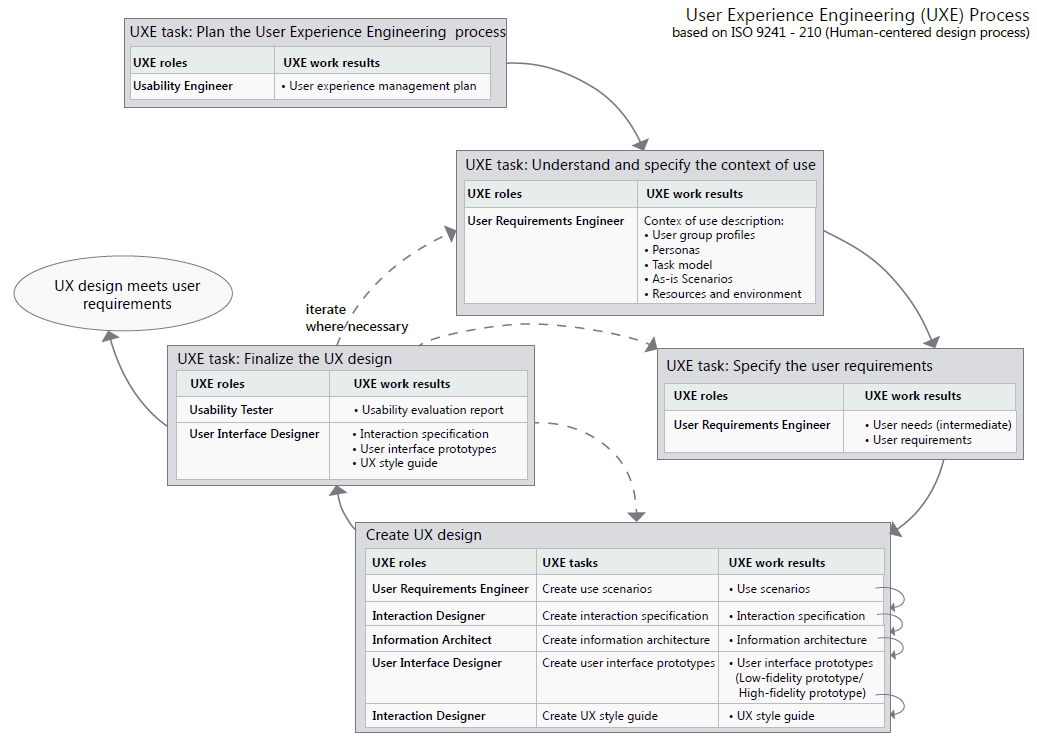
\includegraphics[width=\textwidth]{figures/HCD.png}
  \caption{Human - Centered - Design - Process bei Elektrobit}
  \label{fig:HCD}
\end{center}
\end{figure}

\section{Gestaltprinzipien der Usability}
TODO Notizen fertig machen
TODO Ausformulieren

\cite{Norman.2016} Für Einleitung etwas suchen

\subsection{Konsistenz}
Systeme sind benutzbarer wenn gleiche Funktionen auch die gleiche Darstellung haben.
Ermöglicht es bereits Gelerntes im neuen Kontext anzuwenden, dadurch schnell neue Fähigkeiten zu lernen, und den Fokus auf relevante neue Aspekte zu legen.

Ästhetische Konsistenz bezieht sich auf den Stil und Aussehen, z.B eines Logos. 

Funktionale Konsistenz bezieht sich auf die Konsistenz von Bedeutung und Aktion, z.B Ampel zeigt orange bevor sie rot wird. Erhöht die Usability und Lernfähigkeit, durch Übertragung bereits erlangten Wissens in die neue Umgebung. z.B Playbutton von Kassettenrekorder zu MP3-Player.

Interne Konsistenz bezieht sich auf Konsistenz mit anderen Elementen im System. Erzeugt Vertrauensgefühl bei den Nutzern, vermittelt durchdachtes Design, kein einfaches zusammenstöpseln von Komponenten. Innerhalb einer logischen Gruppen sollten Elemente ästhetisch und funktional Konsistent sein.

Ästhetische und funktionale Konsistenz sollten in allen Designbereichen berücksichtigt werden.
Ästhetische zur Einführung einmaliger Identitäten um Wiedererkennung zu gewährleisten.
Funktionale für gute Usability.
Systeme sollten immer eine interne Konsistenz aufweisen, wenn es bereits Designstandards gibt sollten diese analysiert werden.
\cite{Lidwell.2010}

\subsection{Sichtbarkeit}
Systeme sind benutzbarer wenn der aktuelle Status eindeutig zu erkennen ist, die möglichen Aktionen die ausgeführt werden können, und die Auswirkungen der ausgeführten Aktionen.
Prinzip baut auf der Erkenntnis auf das Menschen Lösungswege erkennen können wenn sie aus einer Anzahl von Optionen auswählen können, als wenn sie sich an einzelne Schritte aus dem Stegreif erinnern müssen.
Für komplexe Systeme ist dieses Prinzip daher das wichtigste für eine gute Usability.
häufig wird versucht alle möglichen Optionen die ein System bietet sichtbar zu machen, was dazu führt das die relevanten Optionen schwerer zu erreichen sind weil eine Informationsüberladung beim Nutzer stattfindet.
Als Lösung bietet sich eine Hierarchische Organisation oder Kontextsensitivität an.
Hierarchische platziert Funktionen und Informationen in logische Kategorien und versteckt sie mit einer übergeordneten Kontrolle, wie zum Beispiel einem Softwaremenü.
Kontextsensitive zeigt oder versteckt Aktionsmöglichkeiten und Informationen abhängig vom aktuellen Status des Systems.
\cite{Lidwell.2010}

\subsection{Affordanz}
Visuelle Eigenschaft eines Elementes das dem Nutzer vermittelt wie mit ihm interagiert werden kann. Im digitalen Umfeld z.B. ein Button.
Ästhetische Eigenschaften eines Buttons müssen visuell vermitteln das er angeklickt werden kann.
Kann visuell gelöst werden indem der Button wie ein Button in der echten Welt aussieht, also ein dreidimensionales Aussehen gewählt wird.
Oder indem der Button komplett anders als der Rest des Interfaces gestaltet wird damit der User versteht das hier eine Interaktion stattfinden kann.\cite{Knight.2019c}

\subsection{Rückmeldung}
Eine Rückmeldung nach der Interaktion eines Nutzers, verdeutlicht diesem das die von ihm beabsichtigte Aktion ausgeführt wurde, ob sie erfolgreich war oder nicht ändert nichts an der Tatsache das eine Rückmeldung nötig ist.
Kommt gar keine Rückmeldung vom System kann der Nutzer nicht zuordnen ob überhaupt eine Aktion ausgeführt wurde. Durch fehlende Rückmeldungen kommt Misstrauen beim Nutzer auf, weil ihm nicht vermittelt wird ob auf seine Aktionen auch eine Reaktion des Systems erfolgt.\cite{Knight.2019c}

\subsection{Mapping}
Wenn der Effekt den eine Nutzerinteraktion nach sich zieht, den Erwartungen des Nutzers entspricht, handelt es sich um gutes Mapping. Beispiel elektronisches Fensterheber, Hebel nach oben hebt das Fenster, Hebel nach unten senkt es.

Gutes Mapping ist zum Großteil eine Funktion der Ähnlichkeit eines Layouts, dessen Verhaltens, oder dessen Bedeutung.
Layout Herdplattenregler entspricht der Anordnung der Platten -> Layout
Bewegung Lenkrad -> Verhalten
Notfallknopf in der Farbe rot -> Bedeutung
In jedem dieser Fälle macht die Ähnlichkeit es möglich den Effekt der Handlung vorherzusehen, vereinfacht also die Bedienung.

Aktionsmöglichkeiten müssen so platziert werden das ihre Position und ihr Verhaltend dem Layout und dem Verhalten den Anwendung angepasst sind. Simple Beziehungen zwischen Eingabe und Aktion funktionieren am besten.
Die gleiche Aktion für verschiedene Funktionen zu benutzen sollte vermieden werden.
\cite{Lidwell.2010}
\subsection{Einschränkungen}
Einschränkung der Aktionen die ein Systems ausführen kann, z.B. ausgrauen von Buttons die nicht funktionstüchtig sind.
Richtige Anwendung von Einschränkungen macht ein Design einfacher nutzbar und reduziert deutlich die Wahrscheinlichkeit von Fehlschlägen während der Systeminteraktion.
Zwei Typen von Einschränkungen: Physische und Psychologische \cite{Lidwell.2010}

Mehr bei \cite{Norman.2016}
\subsection{Vorteile für den Nutzer}
Durch die Nutzung bekannter Interfacestrukturen und Funktionalitäten, muss der Nutzer seine Energie nicht darauf verschwenden darüber nachzudenken wie mit den Bestandteilen des Interfaces interagiert werden kann, oder was deren Funktion sein könnte.
\cite{Knight.2019c}

\section{EB Guide Studio}
Wie bereits in Abschnitt 1.2 erwähnt dient EB GUIDE der Entwicklung multimodalder HMIs.
Um nicht nur das Design sondern auch das Verhalten von User Interfaces bestimmen zu können und eine Auslieferung auf das Zielsystem zu ermöglichen besteht die Produktlinie EB GUIDE aus den verschiedenen, in \cref{fig:guide_puzzle} zu sehenden, Komponenten.
Hierbei wird zwischen Komponenten für das Graphical User Interface (GUI) und Komponenten für die Sprachsteuerung unterschieden.
Da die Sprachkomponenten jedoch für diese Arbeit nicht weiter relevant sind werden diese in den folgenden Kapiteln auch nicht genauer erläutert.
Innerhalb des GUI Bereiches bildet EB GUIDE Studio das tatsächliche Modellierungstool mit dem das Verhalten und Aussehen der Benutzeroberfläche definiert wird.
Für das entwickelte Modell stellt das EB GUIDE Target Framework auf dem Zielsystem die Laufzeitumgebung bereit.\cite{.c} 

\begin{figure} [!h]
\begin{center}
  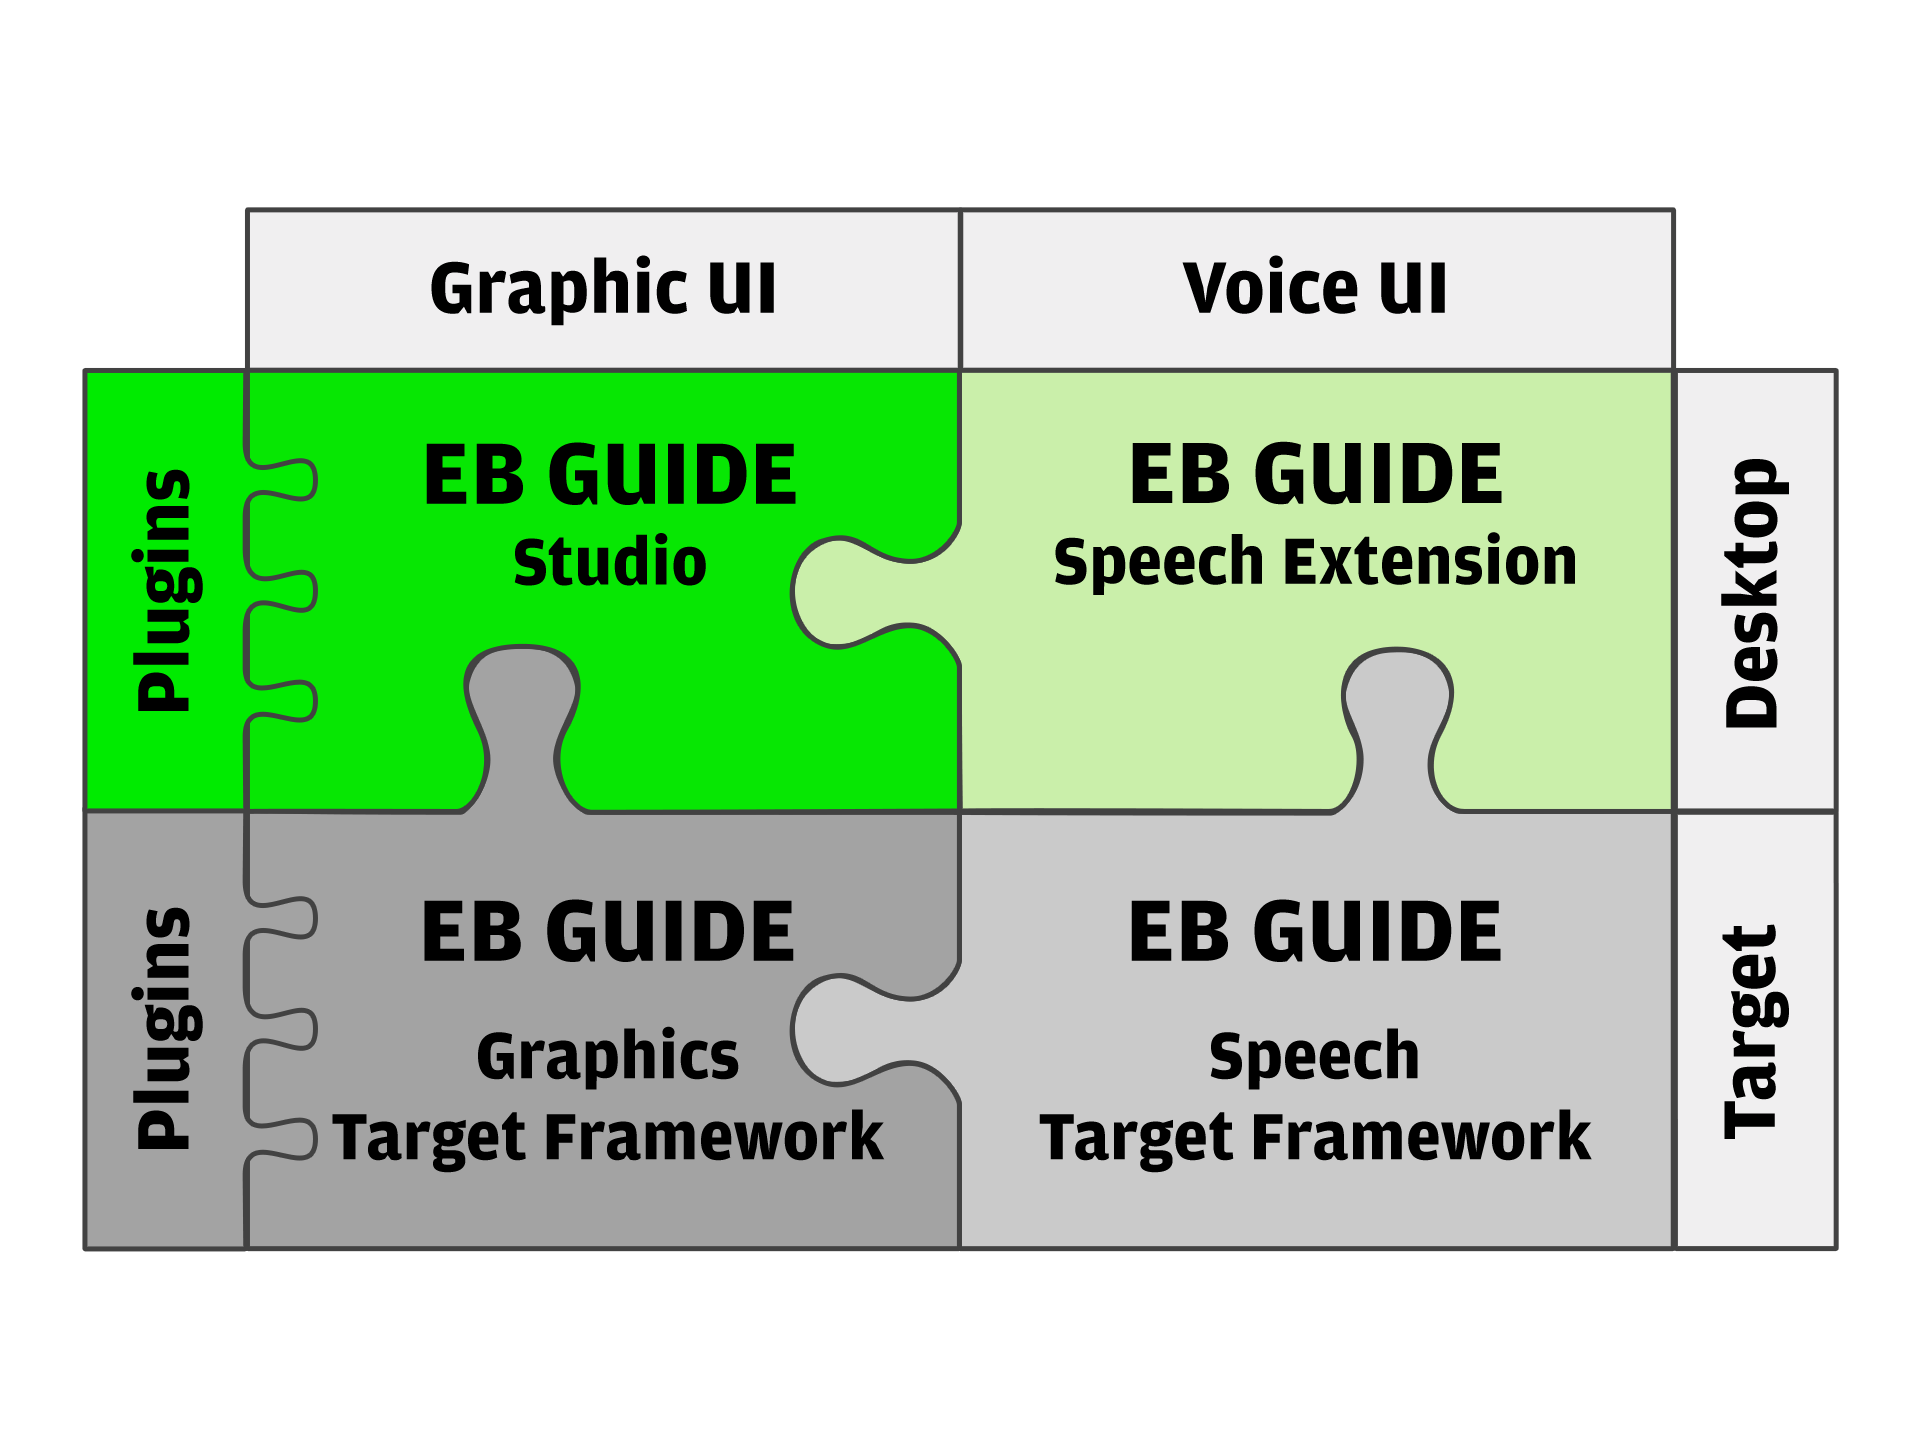
\includegraphics[scale=0.7]{figures/EB_GUIDE_Puzzle.png}
  \caption{Aufbau EB GUIDE}
  \label{fig:guide_puzzle}
\end{center}
\end{figure}

EB Guide Studio ist das Interface von EB Guide mit dem nach dem What-You-See-Is-What-You-Get (WYSIWYG) Prinzip User Interfaces modelliert werden. 
Durch das WYSIWYG Prinzip ist es während des Modellierens einer View bereits möglich das Endergebnis des Designs zu sehen.
Das Verhalten des Interfaces hingegen wird mithilfe einer Zustandsmaschine, der sogenannten Statemachine, modelliert die auf dem UML- Prinzip aufbaut.
Die Trennung der Logik und des Designs wird in EB GUIDE Studio grafisch durch zwei unterschiedliche Arbeitsoberflächen gestaltet in welchen den Modellierern jeweils die entsprechenden Tools und Elemente zur Verfügung stehen.

\begin{figure} [!h]
\begin{center}
  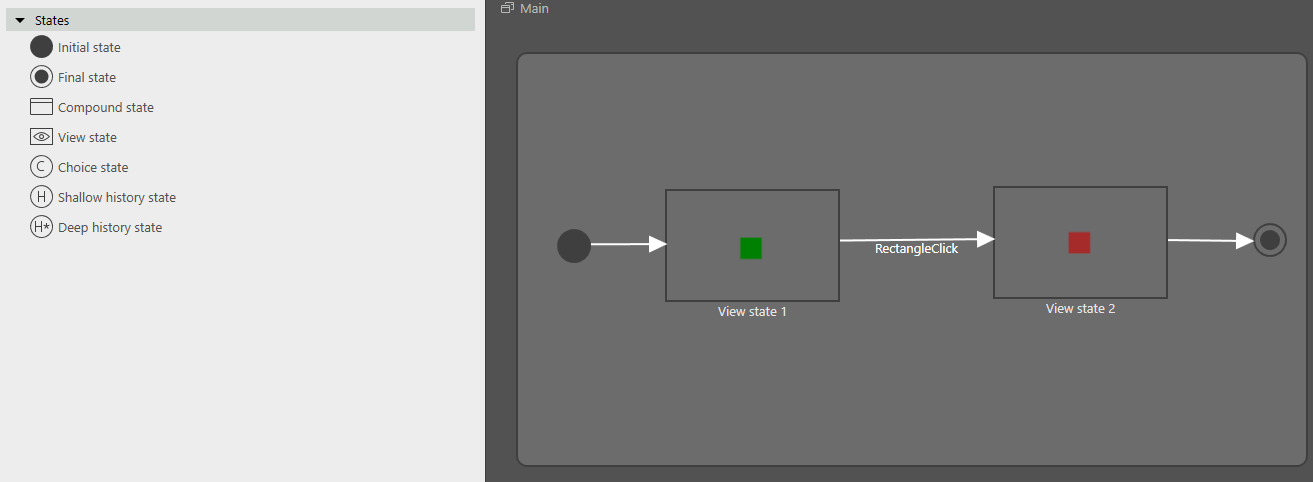
\includegraphics[scale=0.4]{figures/Guide_Statemachine.PNG}
  \caption{EB Guide Studio Statemachine}
  \label{fig:Guide_Statemachine}
\end{center}
\end{figure}

In \cref{fig:Guide_Statemachine} ist die Statemachine für ein simples Beispiel zu sehen.
Links neben der Arbeitsfläche befindet sich eine Toolbox mit deren Inhalt per Drag and Drop auf der Arbeitsfläche die benötigte Logik definiert wird.
Wie bei UML-Diagrammen gibt es einen Initial State der den Startpunkt angibt und einen Final State der die Statemachine beendet.
Die ebenfalls zu sehenden View States stehen für einen Screen im Endprodukt, dementsprechend wird in den View States auch das Aussehen der Interfaces definiert.
Die Verbindungen zwischen den States werden als Transitionen bezeichnet und mithilfe von Events ausgelöst.
Events stellen hierbei beliebige Ereignisse dar die durch Elemente in der View ausgelöst werden können.
Der Auslöser für das Event wird mithilfe einer eigens für EB Guide entwickelten Skriptsprache als Trigger für dieses gesetzt.
Die häufigsten Auslöser sind Benutzeraktionen mit Widgets, die in \cref{fig:Guide_View}zu sehen sind.
Widgets sind Elemente mit denen das Aussehen des Interfaces im sogenannten View Editor bestimmt wird und die sich in Basis- und 3D-Widgets einteilen lassen.
Alle Basiswidgets verfügen über Basiseigenschaften wie Höhe, Breite und Farbe sowie über spezifische Eigenschaften wie zum Beispiel "Touch-Released" bei einem Button.\cite{studio_guide}
Beipspielsweise wird das Event "RectangleClick", was sich in \cref{fig:Guide_Statemachine} an der Transition zwischen View State 1 und View State 2 befindet in diesem Beispiel durch das Klicken auf das grüne Rechteck in View State 1 ausgelöst.
Ist die Benutzeraktion abgeschlossen findet der Übergang von View State1 zu View State 2 statt und der Nutzer sieht nun anstatt dem grünen ein rotes Rechteck.
Damit diese Aktion erfolgreich ausgeführt wird muss das grüne Rechteck die Eigenschaft "Touch-Released"\ zugewiesen bekommen und über die EB Guide Skriptsprache mitgeteilt bekommen das Event RectangleClick zu feuern sobald das grüne Rechteck berührt wurde.
Da sich dieses Event in der Statemachine an der Transition zwischen den beiden States befindet wird nun durch einen Klick auf das grüne Rechteck ein Bildschirmwechsel zwischen den beiden View States ausgelöst.

\begin{figure}[!h]
\begin{center}
  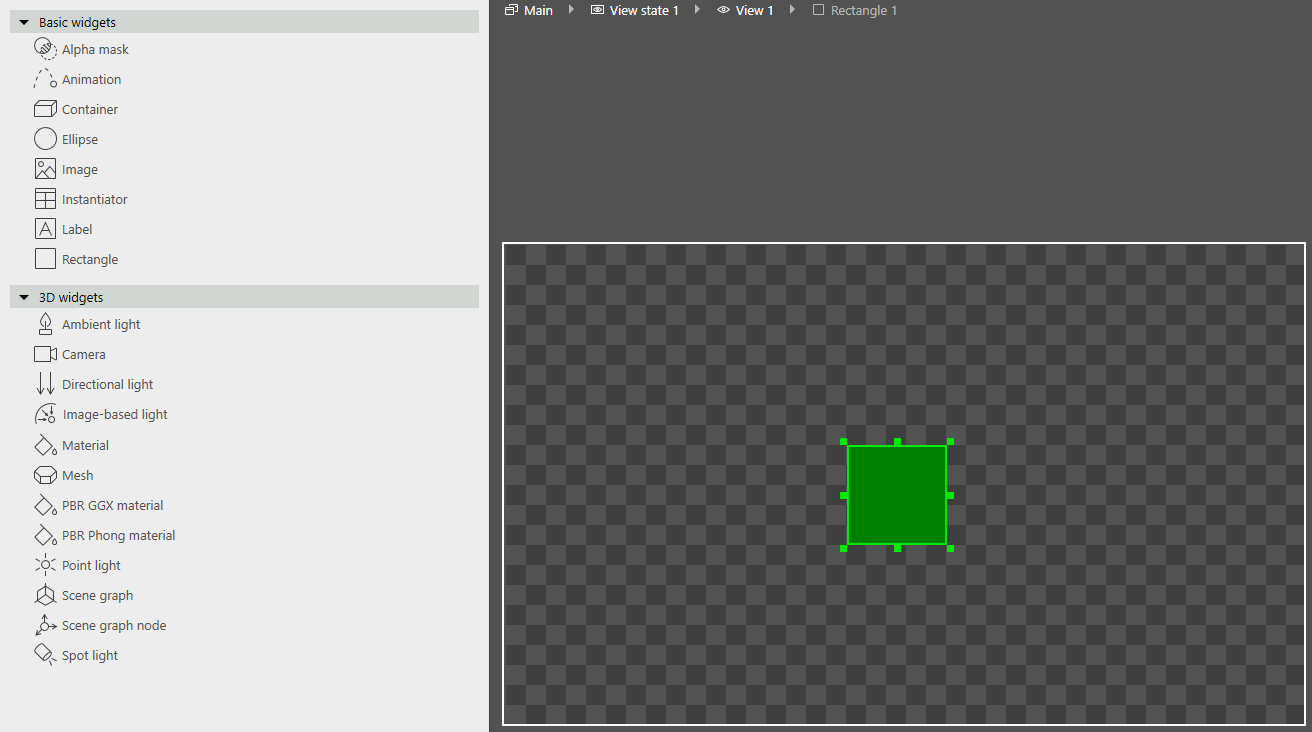
\includegraphics[scale=0.4]{figures/Guide_View.PNG}
  \caption{EB Guide VIEW}
  \label{fig:Guide_View}
\end{center}
\end{figure}



\chapter{Analysen}\label{ch:method}

\section {Voruntersuchungen}
\subsection{Ausgangssituation}
\subsection{Vorgehensweise}
\subsection{Ergebnisse}

\paragraph{Image List}
Jedes Listenelement muss einzeln hinzugefügt werden. Listen haben immer große Dimensionen, unglaublicher Zeitaufwand.

\begin{center}
  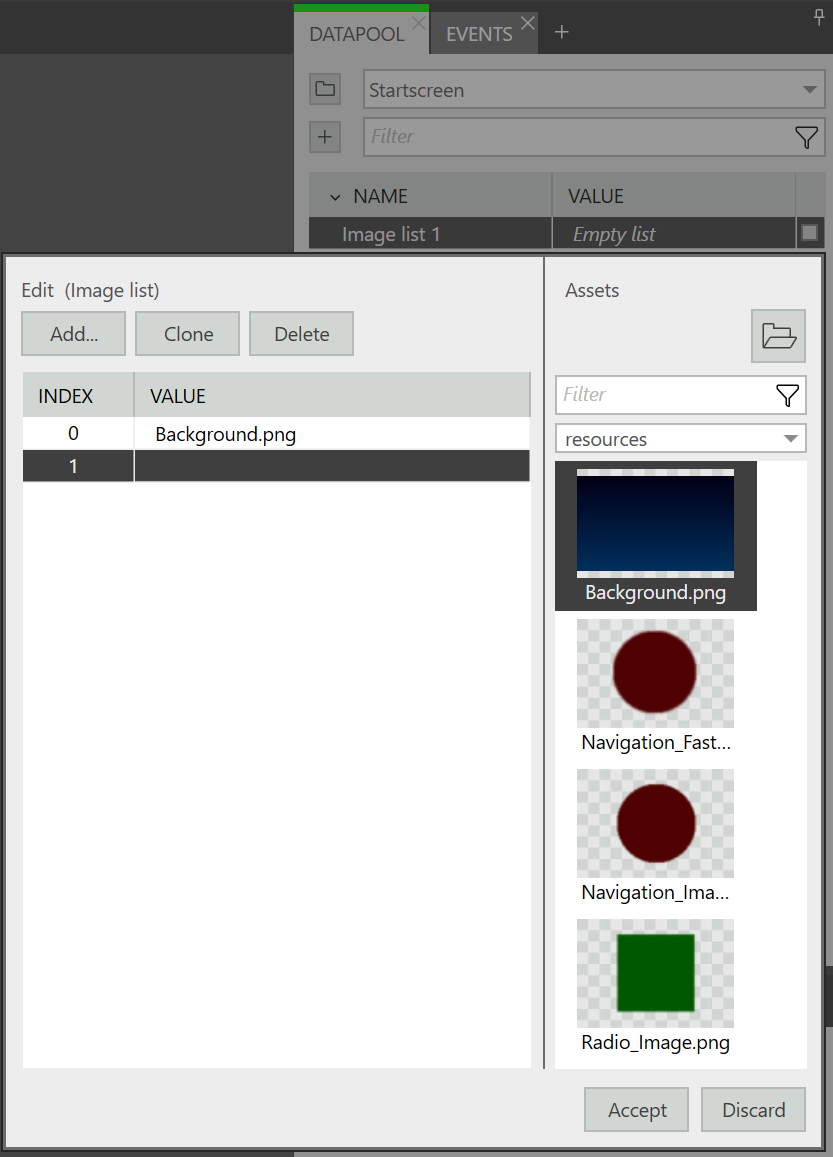
\includegraphics[scale=0.5]{figures/ImageList.png}
  \captionof{figure}{Usability - Schwäche Image List}
  \label{fig:ImageList}
\end{center}


\paragraph{Navigation}
Wird ein neues Element in der View hinzugefügt wird der Baum in der Naviagtion nicht automaisch ausgeklappt. Das Element muss zum umbenennen gesucht werden. Automatisches ausklappen und markieren des eingefügten Objektes zur Umbenennung.

\begin{center}
  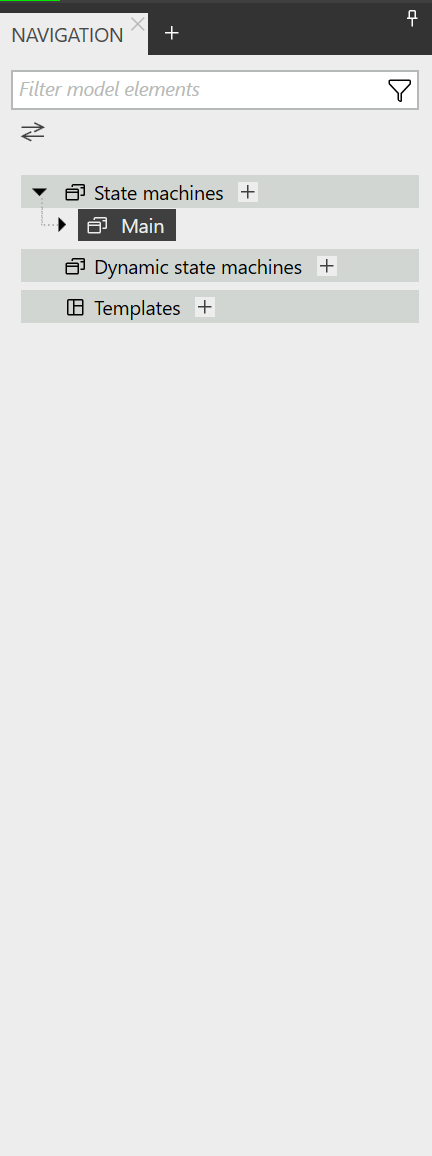
\includegraphics[scale=0.5]{figures/Navigation.png}
  \captionof{figure}{Usability - Schwäche Navigation}
  \label{fig:Navigation}
\end{center}


\paragraph{Template Properties}
Rechtsklick bei Widget Properties notwendig um Verlinkung zum Template Interface zu erstellen. Einfacher klick auf Kreis vorne?

\begin{center}
  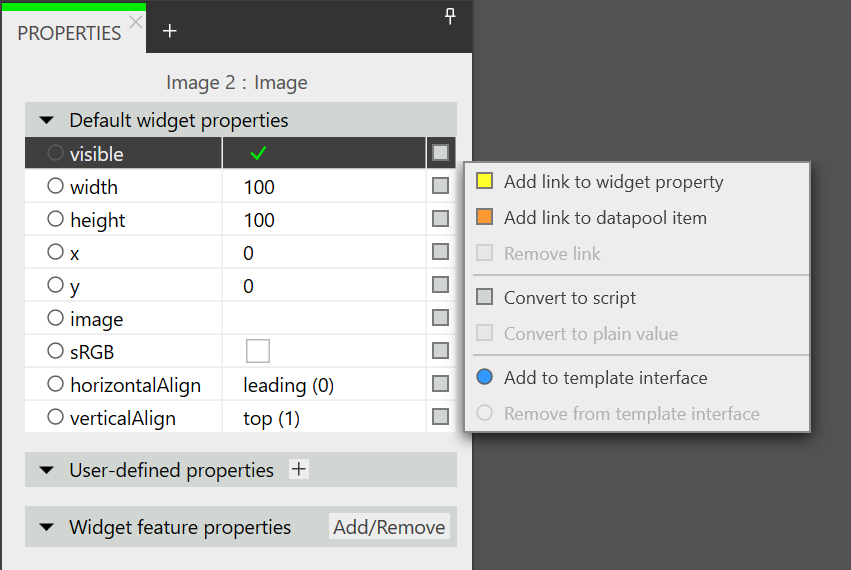
\includegraphics[scale=0.5]{figures/TemplateProperties.png}
  \captionof{figure}{Usability - Schwäche Template Properties}
  \label{fig:TemplateProperties}
\end{center}


\paragraph{Widget Feature Properties}
Häufiges Ausklappen der obermenüs bei der Suche nach bereits bekannten Features. Suche einbauen?

\begin{center}
  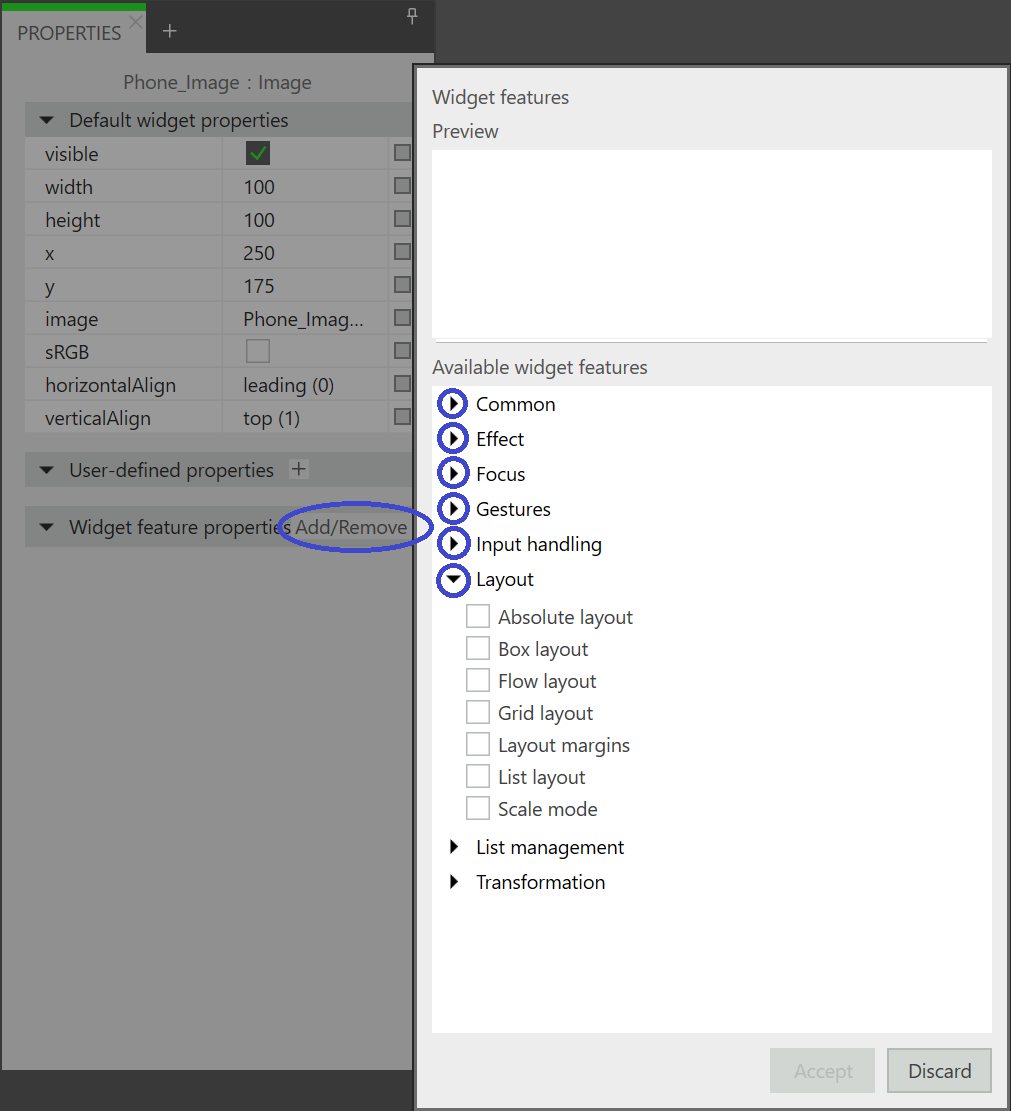
\includegraphics[scale=0.5]{figures/WidgetFeatureProperty.png}
  \captionof{figure}{Usability - Schwäche Widget Feature Properties}
  \label{fig:WidgetFeatureProperty}
\end{center}


\paragraph{Mehrfachselektion}
Bei Mehrfachselektion keine Anpassung der Properties mehr möglich. Im WidgetTree nicht sichbar was ausgewählt ist, hier ist eine mehrfache Markierung auch nicht möglich.

\begin{center}
  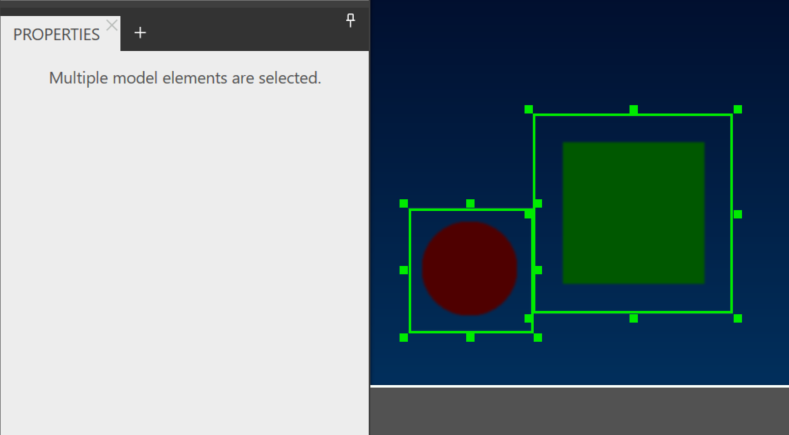
\includegraphics[scale=0.8]{figures/Mehrfachselektion.png}
  \captionof{figure}{Usability - Schwäche Mehrfachselektion}
  \label{fig:Mehrfachselektion}
\end{center}


\paragraph{Default Widget Properties}
Springen zum nächsten Property mit Enter/Pfeiltasten möglich, jedoch keine Markierung zur direkten Bearbeitung.
Auch hier keine Mehrfachselektion möglich, praktisch bei z.B quadratischen Bildern.
\begin{center}
  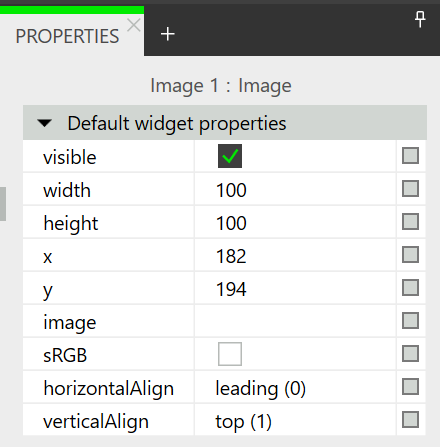
\includegraphics[scale=0.8]{figures/DefaultProperties.png}
  \captionof{figure}{Usability - Schwächen bei den Default Widget Properties}
  \label{fig:DefaultProperties}
\end{center}


\section{Verbesserungen}
\subsection{Auswahlkriterien}
\subsection{Gewinn für den Nutzer}
\subsection{Design der Verbesserungen}

\paragraph{Navigation}

\begin{center}
  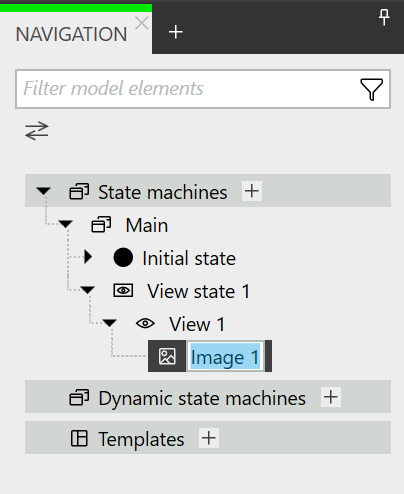
\includegraphics[scale=0.8]{figures/Navigation_Adaption.png}
  \captionof{figure}{Verbesserung Navigation}
  \label{fig:Navigation_Adaption}
\end{center}


\paragraph{Template Properties}

\begin{center}
  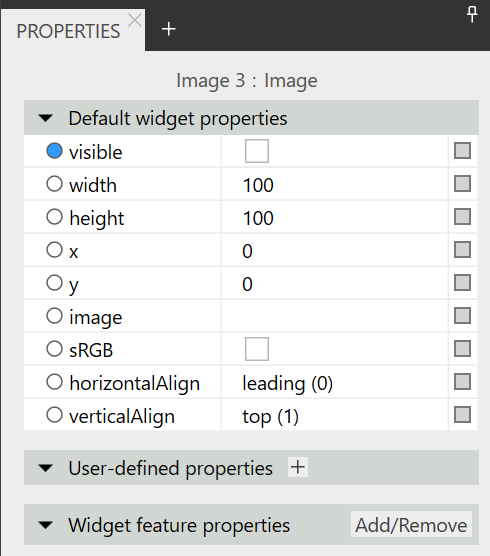
\includegraphics[scale=0.8]{figures/TemplateProperties_Adaption.png}
  \captionof{figure}{Verbesserung Template Properties}
  \label{fig:TemplateProperties_Adaption}
\end{center}


\paragraph{Widget Feature Properties}

\begin{center}
  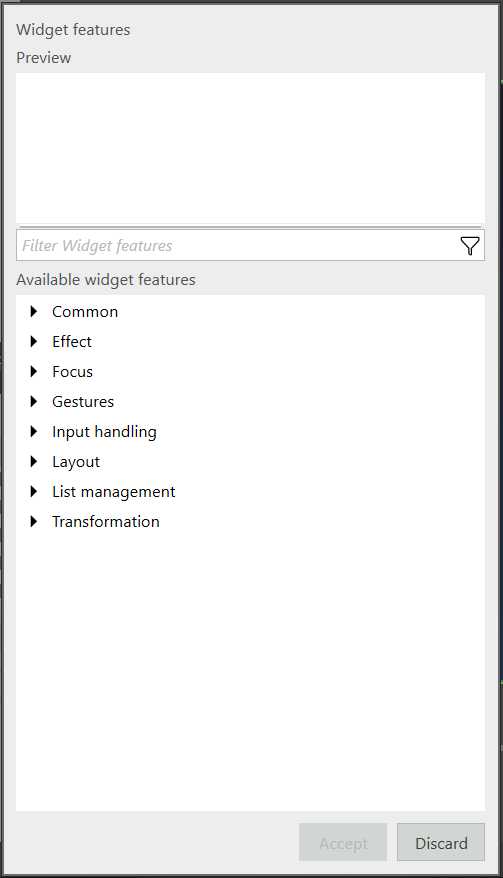
\includegraphics[scale=0.4]{figures/WidgetFeatureProperty_Adaption.png}
  \captionof{figure}{Verbesserung Feature Property Properties}
  \label{fig:FeatureProperty_Adaption}
\end{center}


\paragraph{Mehrfachselektion}

\begin{center}
  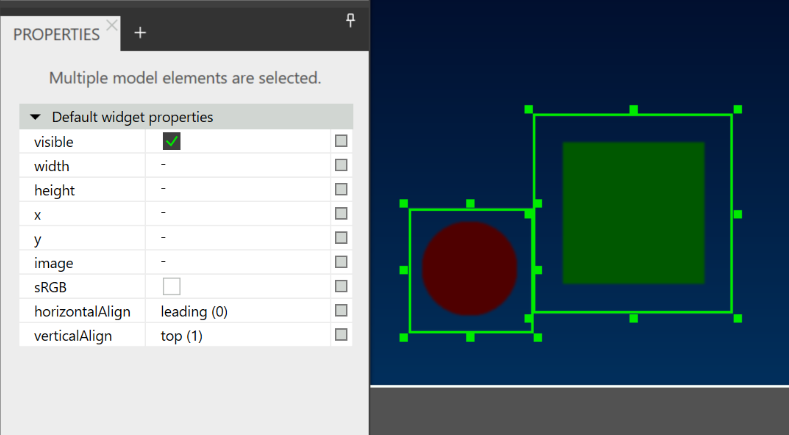
\includegraphics[scale=0.4]{figures/Mehrfachselektion_Adaption.png}
  \captionof{figure}{Verbesserung Mehrfachselektion}
  \label{fig:Mehrfachselektion_Adaption}
\end{center}


\paragraph{Default Widget Properties}

\begin{center}
  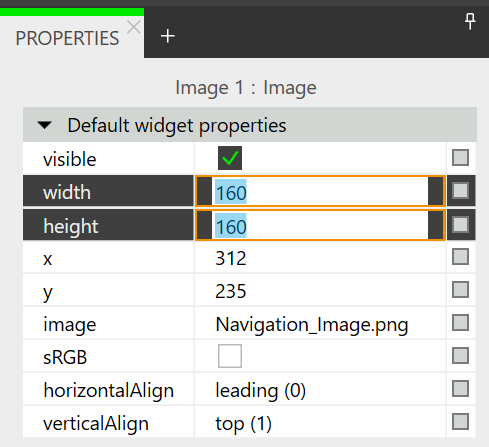
\includegraphics[scale=0.4]{figures/DefaultProperties_Adaption.png}
  \captionof{figure}{Verbesserung Default Widget Properties}
  \label{fig:DefaultProperties_Adaption}
\end{center}

\chapter{Umsetzung}\label{ch:experiments}

Nach Abschluss der Spezifikation der Benutzeranforderungen wird nun in den dritten Schritt des Human-Centered Design Process übergegangen.
Hier gilt es, dass UX Design zu erstellen, wobei der Styleguide bereits am Ende des letzten Kapitels fertiggestellt wurde.
In den folgenden Abschnitten werden noch die benötigten Interaktionsmöglichkeiten definiert und ein, auf diesen Erkenntnissen aufbauender Prototyp erstellt.

Der Großteil der Anpassungen wird in Form eines Prototypen umgesetzte, um weitere Evaluierungen leichter durchführen zu können und um eventuelle Anpassungen innerhalb kommender Iterationen leichter umsetzen zu können.
Konkret werden die große Anpassung der Multiselektion und die kleine Änderunge für die Template Properties innerhalb des Prototypen umgesetzt und untersucht, der Filter für die Widget Feature Properties hingegen wird direkt im EB GUIDE Projekt implementiert.
Dies hat den Hintergrund, dass es bei der Multiselektion absehbar ist, dass hier noch einige Anpassungen nötig sein werden, bis das Design und die Funktionalität an die Bedürfnisse der Nutzer angepasst sind.
Das liegt vor allem daran, dass hier noch keinerlei Grundlagen in EB GUIDE vorhanden sind, auf denen aufgebaut werden kann.
Bei den Template Properties hat die Umsetzung innerhalb des Prototypen den Hintergrund, dass hier nicht sicher gesagt werden kann, ob die Verlagerung der Funktion \glqq publish to template interface\grqq{} von den Nutzern tatsächlich angenommen oder überhaupt an der angedachten Stelle intuitiv erwartet wird.
Es ist hier auch sehr wahrscheinlich, dass an der Darstellung, Positionierung und der Kombination mit der bisherigen Position noch einige Anpassungen stattfinden müssen.
Daher ist es sinnvoll, sich in diesem Fall strikt an den Human-Centered Design Process zu halten und innerhalb dessen Iterationen, solange das UX Design zu verbessern bis es sicher den Nutzeranforderungen entspricht.
Ansonsten würde hoher Entwicklungsaufwand in Anpassungen fließen die noch häufig verändert oder komplett verworfen werden müssen.
Die Anpassung des Prototypen kann in diesen Fällen schneller, minimalistischer und mit kleinerem Aufwand erfolgen.

Im Gegensatz dazu macht es Sinn die Filterfunktion direkt in EB GUIDE zu implementieren.
Aus den bereits durchgeführten Analysen geht hervor, dass dieser Filter einen großen Mehrwert für die Nutzer bieten würde.
Im Gegensatz zu den beiden anderen Änderungen gibt es hier keinen großen Spielraum mehr für Anpassungen, da sich das Design an den bereits bestehenden Filter und Suchfunktionen innerhalb von EB GUIDE orientiert.
Die einzige eventuelle Anpassung die hier noch auftreten könnte, wäre eine Änderung der Position.
Ob dies jedoch innerhalb eines Prototypen oder im Code stattfindet, macht - betrachtet man den zeitlichen Aufwand - keinen Unterschied.
Daher ist es hier effizienter, die Änderungen direkt zu implementieren und das Verhalten nicht zuerst innerhalb eines Prototypen zu simulieren.

\section {Prototyp Multiselektion und Template Properties}
In den folgenden Abschnitten werden alle relevanten Aspekte im Bezug, auf die im Prototyp umgesetzten Änderungen erläutert.
Zuerst folgt eine kurze Begründung für die Wahl des Prototyping Tools.
Da für diese Arbeit eine Einarbeitung in dieses Tool erfolgt ist, wird dieses darauf folgend in seinen Grundfunktionen erläutert.
Dies ist auch notwendig um die abschließend dargestellte Vorgehensweise zur Erstellung des Prototyps nachvollziehen zu können.
Danach werden die nötigen Interaktionsmöglichkeiten definiert, die dem Nutzer für einen erfolgreichen Umgang mit dem Prototypen simuliert werden müssen, bevor letztlich die Vorgehensweise beschrieben wird um diese Anforderungen umzusetzen.

\subsection {Axure RP}
Axure RP ist eine Software die es ermöglicht Wireframes, Prototypen, Dokumentationen und Spezifikationen für Web-, Mobil- oder Desktopanwendungen zu erstellen.
Dies wird durch Drag and Drop Aktionen, Skalierung und Formatierung von Widgets ermöglicht, mit deren Hilfe man das gewünschte Endprodukt erstellen kann.
Für diese Arbeit ist vor allem die Möglichkeit einen Prototypen zu erstellen wichtig.
Ausschlaggebend für die Wahl dieser Software ist, dass AXURE RP 9 die Möglichkeit bietet dynamische Inhalte zu erstellen und logische Bedingungen in den Prototypen einzubinden.
Da es sich bei EB GUIDE Studio um ein Modellierungstool handelt, ist ein rein statischer Prototyp nicht ausreichend.
Ebenfalls reicht es nicht aus feste Hotspots zu haben bei deren Klick etwas passiert, sondern es ist notwendig, die in EB GUIDE herrschenden Einschränkungen für den Nutzer simulieren zu können.

Ein weiterer Grund sich für diese Software zu entscheiden ist es, dass die UX Designer bei Elektrobit ebenfalls mit AXURE RP arbeitet.
So ist zum einen gewährleistet, dass bei den Usabilitytest keine Schwierigkeiten mit der verwendeten Software auftreten würde, zum anderen ist dadurch gleichzeitig ein Ansprechpartner bei auftretenden Problemen vorhanden.

In \cref{fig:Axure_Full} ist das Standardprojekt von AXURE RP zu sehen, welches die Grundlage eines jeden neuen Projektes bildet.

\begin{center}
  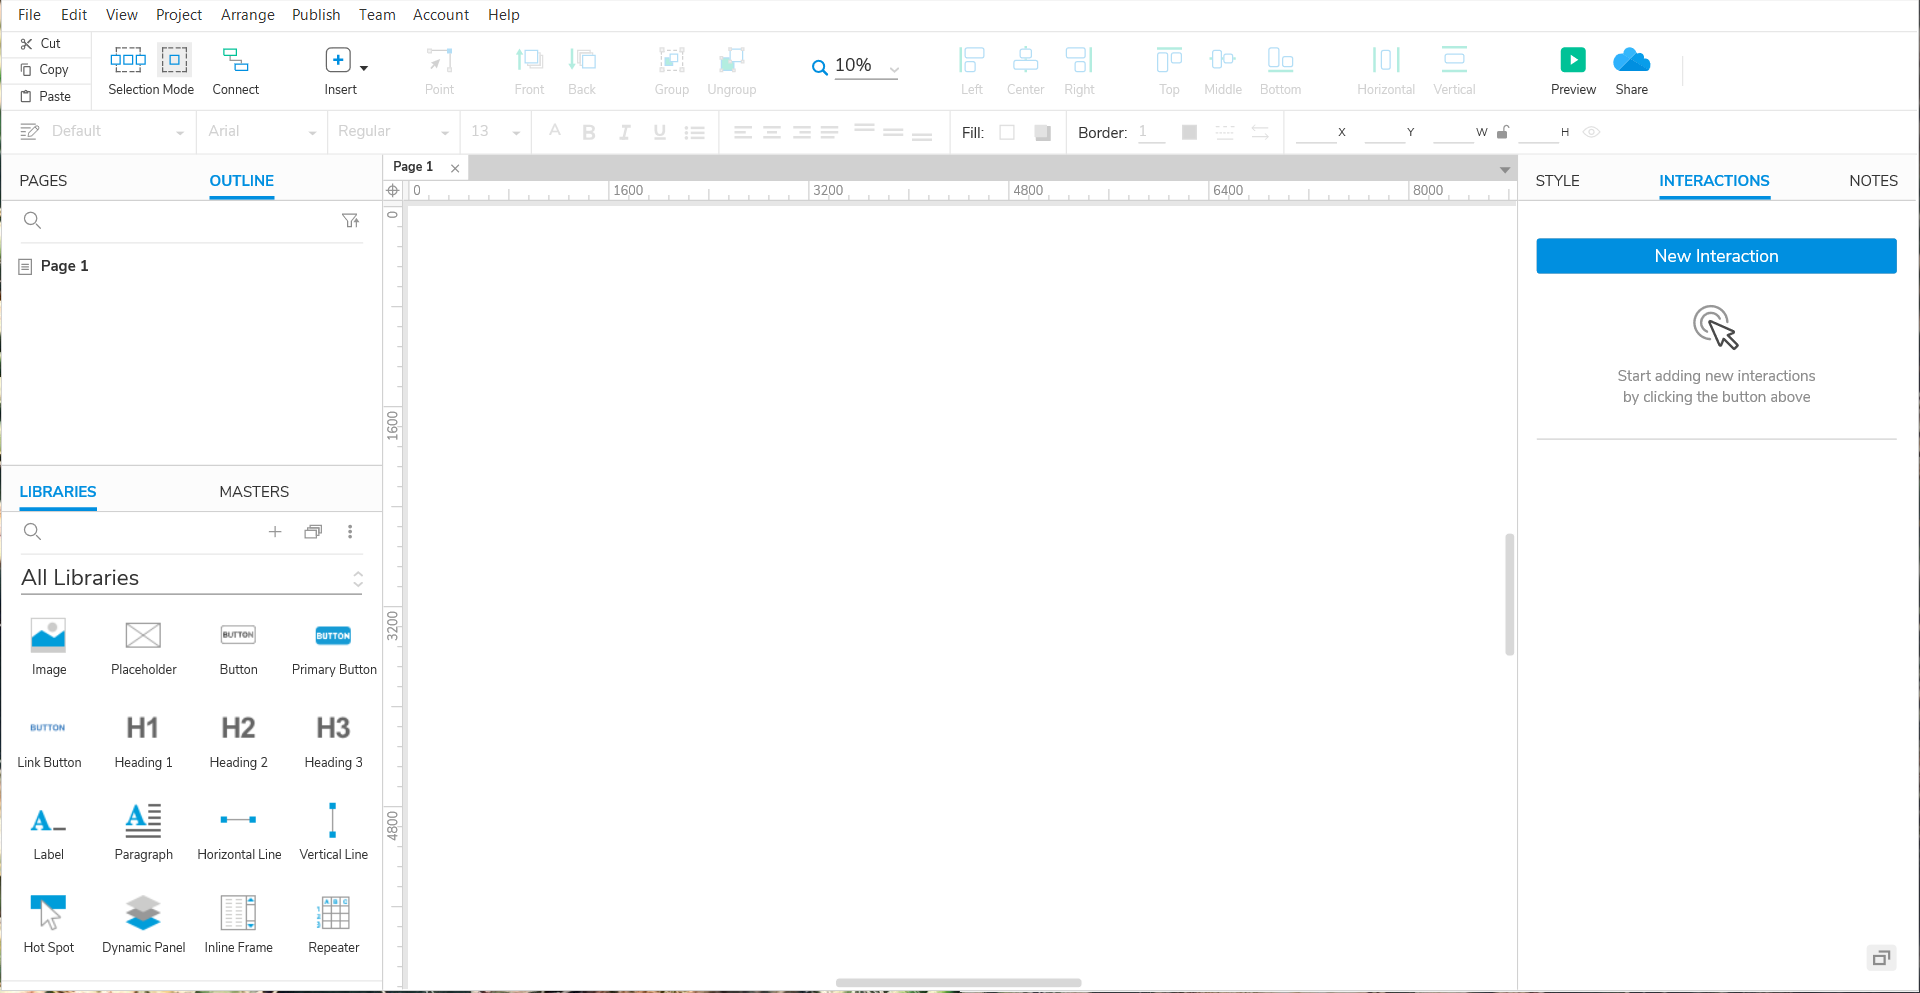
\includegraphics[scale=0.3]{figures/Axure_Full.png}
  \captionof{figure}{Axure RP 9}
  \label{fig:Axure_Full}
\end{center}

In den mittig platzierten Workspace können Elemente aus den Libraries links oder eigene, externe Elemente eingefügt werden.
Zieht man nun beispielsweise eine Droplist und drei Kreiselemente aus den Libraries links in den Workspace, passt sich die Outline wie in \cref{fig:Axure_Outline} zu sehen entsprechend an.
Mithilfe dieser Outline kann man innerhalb des Projektes navigieren, was vor allem praktisch ist wenn sich mehrere Elemente überlagern.
Elemente lassen sich auch zu Dynamic Panels gruppieren, was vor allem dann nötig ist, wenn man ein Drag und Drop Verhalten simulieren möchte, da dies die einzigen Widgets sind die dieses Verhalten unterstützen.

\begin{center}
  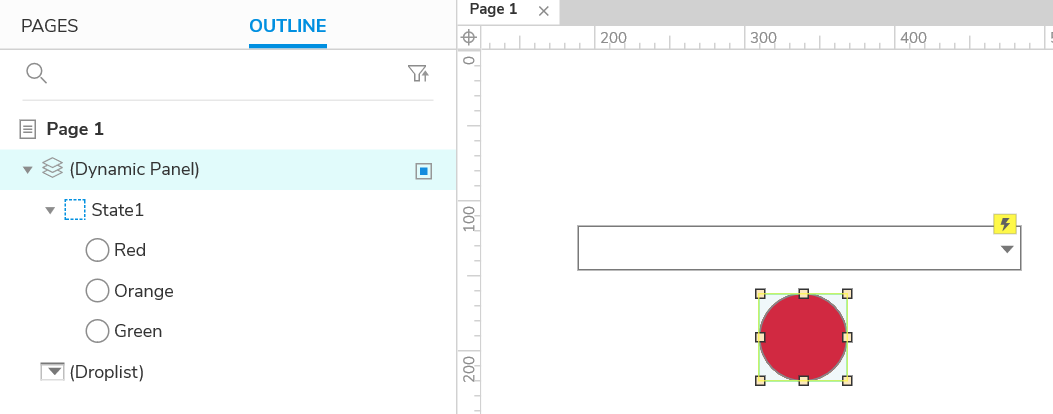
\includegraphics[scale=0.4]{figures/AXURE_Outline.PNG}
  \captionof{figure}{Axure RP 9 Outline}
  \label{fig:Axure_Outline}
\end{center}

Um den drei eingefügten Kreisen unterschiedliche Farben zuzuweisen ist es nötig deren Properties zu bearbeiten.
Dies ist in AXURE RP über das Stlye Panel möglich, welches in \cref{fig:Axure_Style} zu sehen ist.
Hier ist es beispielsweise ebenfalls möglich Skalierungen vorzunehmen oder Umrandungen und Schatten hinzuzufügen.

\begin{center}
  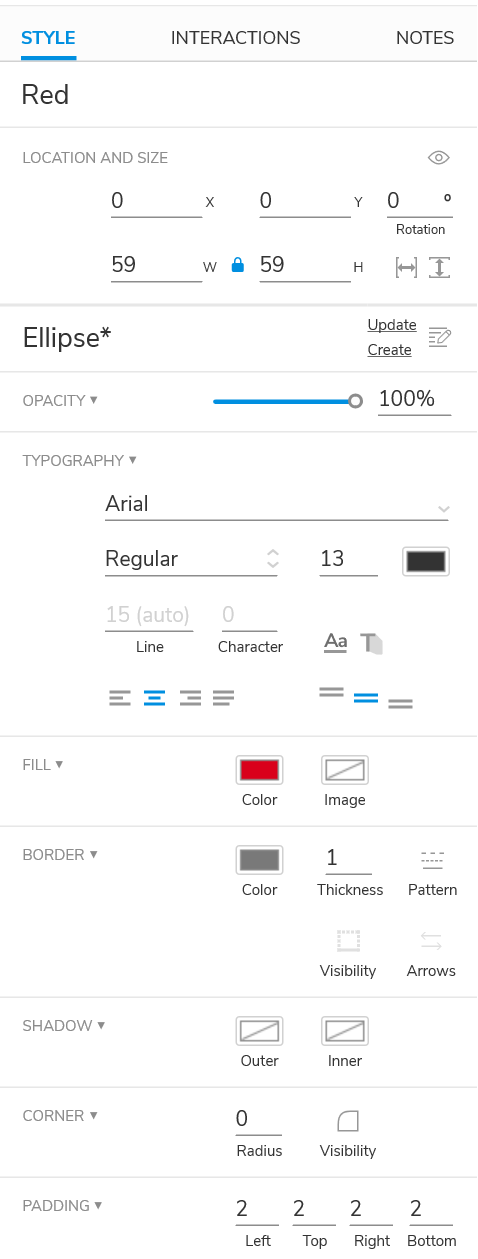
\includegraphics[scale=0.4]{figures/AXURE_Style.PNG}
  \captionof{figure}{Axure RP 9 Style Properties}
  \label{fig:Axure_Style}
\end{center}

Möchte man nun erreichen, dass die Farbe des sichtbaren Kreises sich an der Auswahl innerhalb der Droplist orientiert, muss Logik zu dem Prototypen hinzugefügt werden.
Zuerst ist es, wie in Teil a von \cref{fig:Droplist} zu sehen, nötig Optionen zu der Droplist hinzuzufügen.
Innerhalb des Interaction Panel besteht dann die Möglichkeit, über IF Conditions abzufragen, welche Option aktuell ausgewählt ist.
Passend dazu wird der Kreis mit der gewünschten Farbe angezeigt, und die Visibility der anderen Kreise entsprechend auf null gesetzt.

\begin{figure}%
\centering
\subfloat[][]{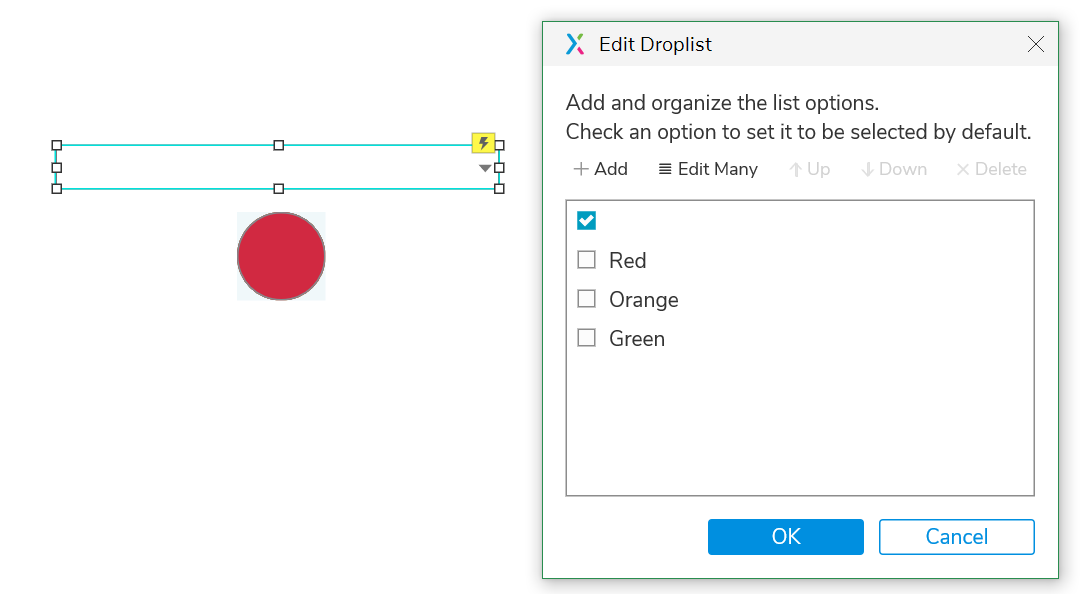
\includegraphics[width=0.3\linewidth]{figures/AXURE_Droplist.PNG}}%
\qquad
\subfloat[][]{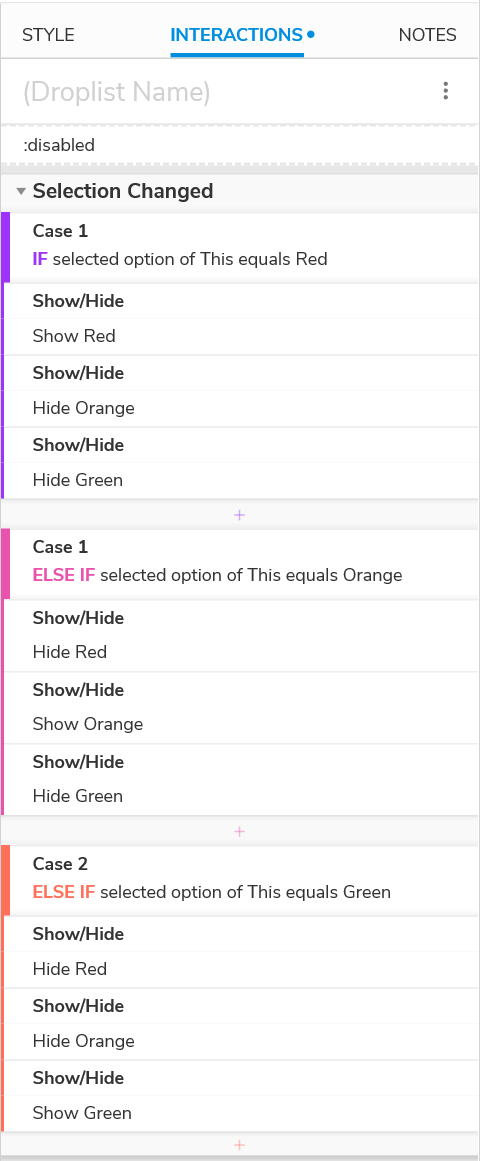
\includegraphics[width=0.3\linewidth]{figures/AXURE_Droplist_Conditions.PNG}}%

\caption{Axure RP Droplist und Conditions}%
\label{fig:Droplist}
\end{figure}

Hat man die Modellierung abgeschlossen, oder möchte Anpassungen überprüfen, bietet AXURE RP die Möglichkeit einer lokalen Preview.
Diese verhält sich exakt so, wie sich der abgeschlossene Prototyp verhalten wird und eignet sich deshalb gut für selbständige Validierung der bisherigen Umsetzung.
Testet man das soeben modellierte Beispiel in der Preview sieht man in \cref{fig:Droplist} , dass sich die Farbe des Kreises, wie gewünscht, immer an die Auswahl der Droplist anpasst.
\begin{figure}%
\centering
\subfloat[][]{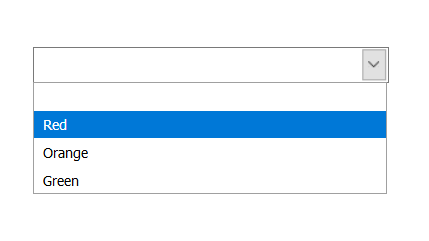
\includegraphics[width=0.3\linewidth]{figures/AXURE_red.PNG}}%
\qquad
\subfloat[][]{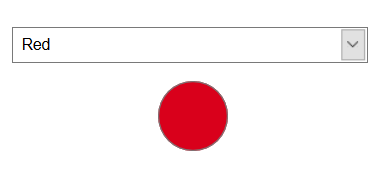
\includegraphics[width=0.3\linewidth]{figures/AXURE_red02.PNG}}%
\qquad
\subfloat[][]{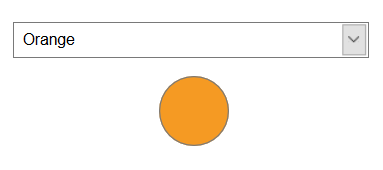
\includegraphics[width=0.3\linewidth]{figures/AXURE_orange.PNG}}%
\qquad
\subfloat[][]{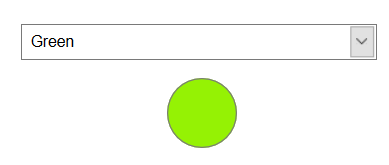
\includegraphics[width=0.3\linewidth]{figures/AXURE_green.PNG}}%

\caption{Axure RP Preview}%
\label{fig:Preview}
\end{figure}

Ist die Modellierung beendet, bietet AXURE RP die Möglichkeit, das Projekt in die AXURE CLOUD zu laden.
Hier können andere Mitarbeiter über einen generierten Link auf das funktionale Endprodukt zugreifen, ohne das eigentliche Projekt sehen oder bearbeiten zu können.
Dadurch ist es nun einerseits möglich andere UX Designer Funktionalitäten des Prototypen testen zu lassen, wobei sie auch an den entsprechenden Stellen Kommentare und TODO's hinterlassen können.
Außerdem besteht durch die Online Verfügbarkeit die Möglichkeit den Prototypen für die Testpersonen im Rahmen des Usability Tests zugänglich zu machen.

\subsection{Interaktionsmöglichkeiten}

Im dritten Schritt des Human-Centered Design Process ist es die Aufgabe des Interaction Designers die Interaktionsmöglichkeiten, die der Prototyp bieten muss, zu spezifizieren.
Dies ist deshalb notwendig, da es gerade bei Prototypen die ein komplexes System simulieren sollen, nicht möglich oder nötig ist alle Funktionen des Systems zu simulieren.
Daher wird vor der Erstellung des Prototyps festgelegt welche Interaktionen von den Nutzern durchführbar sein müssen um die geplanten Verbesserungen validieren zu können.

Für die Prüfung der Usability der Ergänzungen ist es jedoch nicht ausreichend nur die neuen oder ergänzten Funktionen zu simulieren.
Um diese überhaupt anwenden zu können muss der Nutzer einen gewissen Fortschritt innerhalb des Modellierungsprozesses erreicht haben.
Um an diesen Punkt zu gelangen ist es unbedingt notwendig, dass dem Nutzer gewisse Grundfunktionen von EB GUIDE zur Verfügung stehen.
Das bedeutet für den konkreten Fall dieser Bachelorarbeit, dass es für den Nutzer möglich sein muss wie gewohnt Elemente per Drag and Drop in den View zu ziehen, und diese dort auch frei bewegen zu können.
Ebenfalls müssen die Properties aller Widgets frei anpassbar sein und die Elemente müssen wie gewohnt auf die Eingaben des Nutzers reagieren.
Da sich die Funktion \glqq publish to template interface\grqq{} innerhalb der Templates befindet, muss auch die Möglichkeit bestehen Templates anzulegen.

Darauf aufbauend müssen noch die neuen oder veränderten Funktionen in den Prototypen integriert werden.
Dazu zählt konkret, dass die Funktion \glqq publish to template interface\grqq{} verlagert wird und die vorhandene Möglichkeit dafür vorerst nicht simuliert werden muss.
Zusätzlich muss es nun möglich sein, mehrere Elemente gleichzeitig auszuwählen und hierfür ein Property Panel einzublenden.
Die Anpassung der Properties müssen sich in diesem Fall auch auf alle angewählten Elemente auswirken und diese müssen gemeinsam im View bewegt werden können.
Zusätzlich müssen noch die neuen Alignment Actions, sowie die Funktion \glqq Insert in Template\grqq{} angezeigt werden und ausführbar sein.

Da sehr viele unterschiedliche Widget- und Templatetypen in EB GUIDE existieren, ist es an dieser Stelle des Prozesses auch sinnvoll sich bereits Gedanken über den abschließenden Usability Test zu machen und die Funktionen des Prototypen entsprechend einzuschränken.
Die Modellierer bei Elektrobit setzen hauptsächlich HMIs für den Fahrzeuginnenraum mit EB GUIDE um.
Daher erscheint es sinnvoll für den Usability Test einen minimalistischen Startscreen eines solchen Interfaces modellieren zu lassen.
Da diese, wenn man die Interaktionslogik außen vor lässt, nur aus Images und Labels bestehen ist es ausreichend diese beiden Widgets funktionsfähig zu machen.
Zusätzlich dazu ist es noch notwendig die Menge an verfügbaren Templates einzuschränken.
Für den soeben erläuterten Use Case ist es hier ebenfalls ausreichend nur Image Templates erstellen zu können.
Genauere Erläuterungen zu den Aufgaben innerhalb des Usability Test folgen entsprechend in Kapitel 5.


\subsection{Vorgehensweise}
Im folgenden werden die grundlegenden Vorgehensweisen erläutert die angewandt werden, um den Prototypen zu erstellen.
Es ist im Rahmen dieser Arbeit nicht möglich alle exakten Anpassungen zu erläutern die umgesetzt werden.
Es werden jedoch alle maßgeblichen Konzepte und Funktionen aufgeführt die in Zusammenhang mit den eingebauten Neuerungen stehen.
Alle nicht ausführlich erklärten Änderungen sind auf ähnliche Art und Weise umgesetzt, wie solche die in den nächsten Abschnitten erläutert werden.

\paragraph{Grundlage}
Vor allem bei Expertennutzern ist es wichtig, dass der Prototyp sich nicht nur verhält wie die  gewohnte Software, sondern sich auch optisch an ihr orientiert.
Aus diesem Grund ist der Ansatz zur Modellierung des Prototypen, einen Screenshot der aktuellen Version von EB GUIDE Studio zu machen und diesen als statischen Hintergrund, wie in \cref{fig:Prototyp_01} zu sehen, für das weitere Vorgehen zu verwenden.
Darauf aufbauend können nach und nach Interaktionsmöglichkeiten innerhalb des Prototypen platziert werden.

\begin{center}
  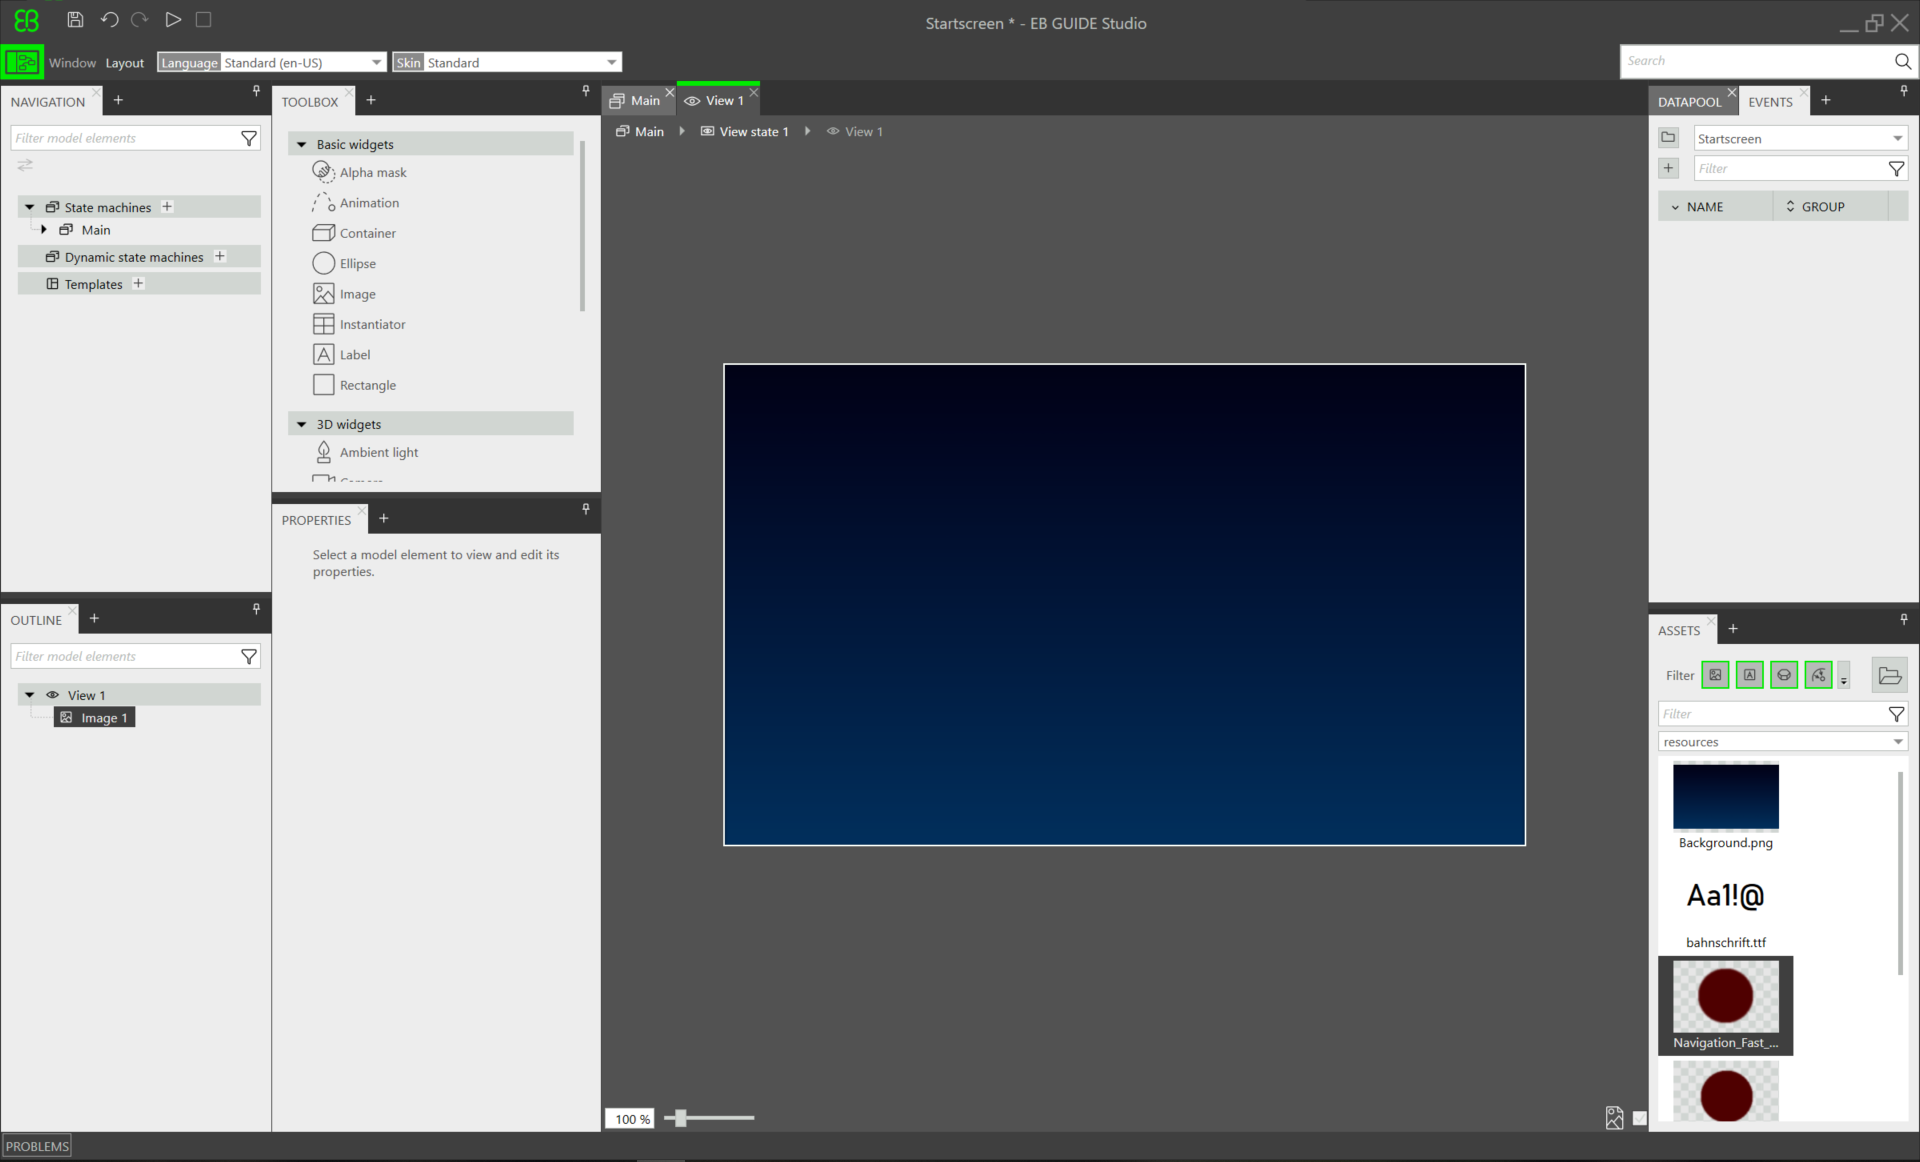
\includegraphics[scale=0.4]{figures/Prototyp_01.PNG}
  \captionof{figure}{Grundlage des Prototyps}
  \label{fig:Prototyp_01}
\end{center}

\paragraph{Assets und Toolbox}
Die Assets und die Toolbox sind wichtige Interaktionsmöglichkeiten für den Nutzer, da von hier alle zur Verfügung stehenden Widgets oder Ressources in den View gezogen werden.
Für beide Elemente wird eine Scrollbar benötigt, da die Nutzer dies an dieser Stelle gewohnt sind, und sonst keine Möglichkeit bestünde alle Widgets und Elemente anzuzeigen.
In AXURE ist es hierfür nötig ein Dynamic Panel zu erstellen und es mit allen benötigten Elementen zu befüllen, die in der Scrollbar vorhanden sein sollen.
Für ein Dynamic Panel ist es möglich eine feste Größe anzulegen, sollten dessen Elemente in der vorgegebenen Dimension nicht alle Platz finden, hat man nun die Möglichkeit Vertikales oder Horizontales Scrolling zu aktivieren.
In \cref{fig:Prototyp_02} sieht man beispielhaft die Umsetzung für das Assetspanel.
Teil a) zeigt die Implementierung mithilfe von ineinander geschachtelter Dynamic Panels, in Teil b) ist das entsprechende Ergebnis im Prototypen zu sehen.

\begin{figure}%
\centering
\subfloat[][]{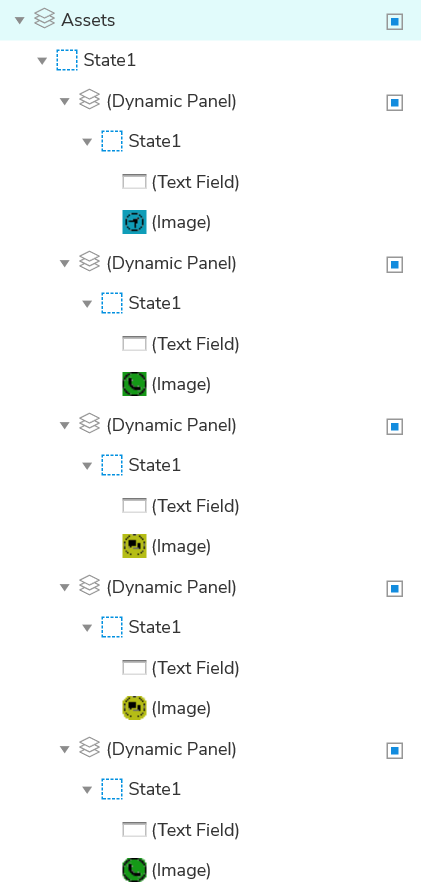
\includegraphics[width=0.4\linewidth]{figures/Prototyp_Assets.PNG}}%
\qquad
\subfloat[][]{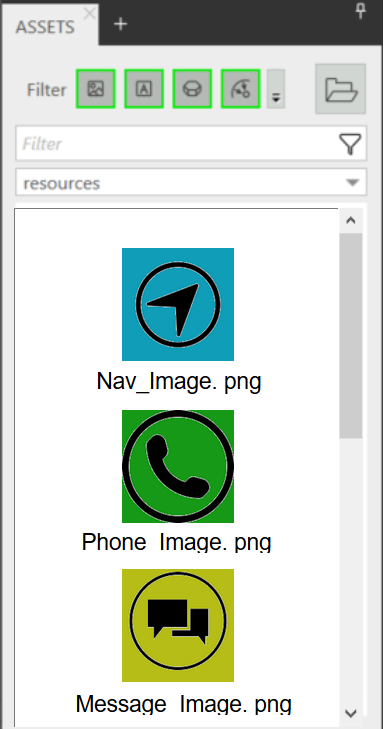
\includegraphics[width=0.4\linewidth]{figures/Prototyp_02.PNG}}%

\caption{Scrollbar für Assets}%
\label{fig:Prototyp_02}
\end{figure}

Der Grund dafür, dass jedes einzelne Bild in den Assets ebenfalls ein Dynamic Panel ist, ist der Tatsache geschuldet, dass dies die einzigen Widgets sind die Drag und Drop unterstützen.
Sie bieten die einzigartigen Interactions \glqq Drag Started\grqq{},\glqq Dragged\grqq{} und \glqq Drag Dropped\grqq{} über welche gesteuert werden kann, wie sich die Items während des Vorgangs verhalten.
Hier erweist es sich als praktisch \glqq Drag Dropped\grqq{} mit einer If Bedingung zu versehen, damit das Element nur über dem dafür vorgesehenen View abgelegt werden kann und nicht zum Beispiel im Bereich der Datapoolitems.

\paragraph{Widget Tree}
Sobald etwas in den View hinzugefügt wird, muss dies für den Nutzer ebenfalls im Widget Tree sichtbar werden.
Dies ist mithilfe eines Screenhots gelöst - zu sehen in \cref{fig:Prototyp_03} -  wobei sich noch weitere Elemente im Widget Tree befinden, die vorläufig überdeckt werden.
Fügt der Nutzer nun das entsprechende Element zum View hinzu, wird die Abdeckung entfernt und das Objekt kann nun über den Widget Tree ausgewählt werden.
Die Interaktionsmöglichkeit wird von AXURE mit den gelben Blitzen gekennzeichnet und ist ebenfalls mit logischen Bedingungen umgesetzt.

\begin{center}
  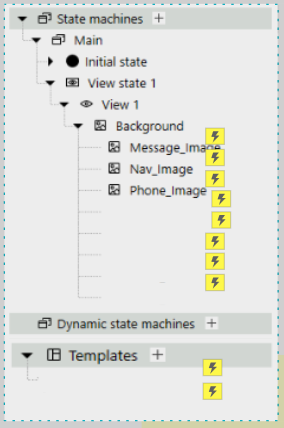
\includegraphics[scale=0.8]{figures/Prototyp_03.PNG}
  \captionof{figure}{Widget Tree}
  \label{fig:Prototyp_03}
\end{center}

\paragraph{Properties}
Um die Interaktion mit allen eingefügten Elementen möglich zu machen, erhält jedes Element sein eigenes Property Panel, welches in \cref{fig:Prototyp_04} zu sehen ist.
Damit dem Nutzer immer klar ist, welches Element aktuell ausgewählt ist, wird auch hier das Verhalten von EB GUIDE nachgebaut, indem jedes ausgewählte Element einen grünen Rahmen erhält.
Die Auswahl hierfür muss über das Element selbst oder den Widget Tree möglich sein.

Ist das Objekt aktuell ausgewählt erscheint ein entsprechendes Property Panel, welches ebenfalls einen Screenshot beinhaltet der mit Textfeldern überlagert wird.
Diese Felder sind mit globalen Variablen verknüpft, welche wiederum die Properties der Bilder im Workspace von AXURE anpassen.
Dadurch wird es ermöglicht, dass Eingaben in das Textfeld das Objekt verändern und umgekehrt, Bewegungen des Objektes die Werte in den Textfeldern aktualisieren.
Damit wird für den Nutzer das exakt gleiche Verhalten nachmodelliert, welches in EB GUIDE existiert.
Ein identisches Verhalten ist für die Texte modelliert, nur haben diese statt eines Image Properties ein Text Property.

\begin{center}
  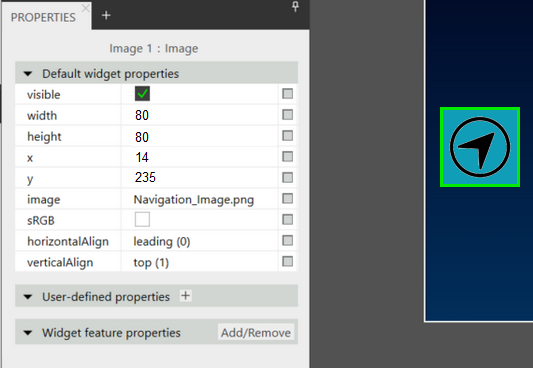
\includegraphics[scale=0.8]{figures/Prototyp_04.PNG}
  \captionof{figure}{Properties Panel}
  \label{fig:Prototyp_04}
\end{center}

\paragraph{Multiselektion}
Ist nur ein Objekt ausgewählt wird der Wert der globalen Variable im entsprechenden Textfeld angezeigt.
Dieser Wert soll bei der Multiselektion jedoch nur angezeigt werden, wenn er für alle ausgewählten Objekte identisch ist.
Da ansonsten ein Strich sichtbar sein soll, ist es hier notwendig die Properties der ausgewählten Objekte zu vergleichen.
Hierfür muss zuerst abgefragt werden welche Objekte ausgewählt sind, um dann deren Properties zu vergleichen.
Da AXURE bei den logischen Bedingungen nur \glqq Match Any\grqq{} oder \glqq Match All\grqq{} unterstützt ist keine Kombination von AND und OR Bedingungen möglich.
Deshalb wird an diesem Punkt nur mit AND Bedingungen in den Abfragen gearbeitet, da jedoch für alle möglichen Kombinationen der drei zur Verfügung stehende Bildern jede Property einzeln abgefragt und angepasst werden muss, ergibt das eine Anzahl von 36 Abfragen.

\begin{center}
  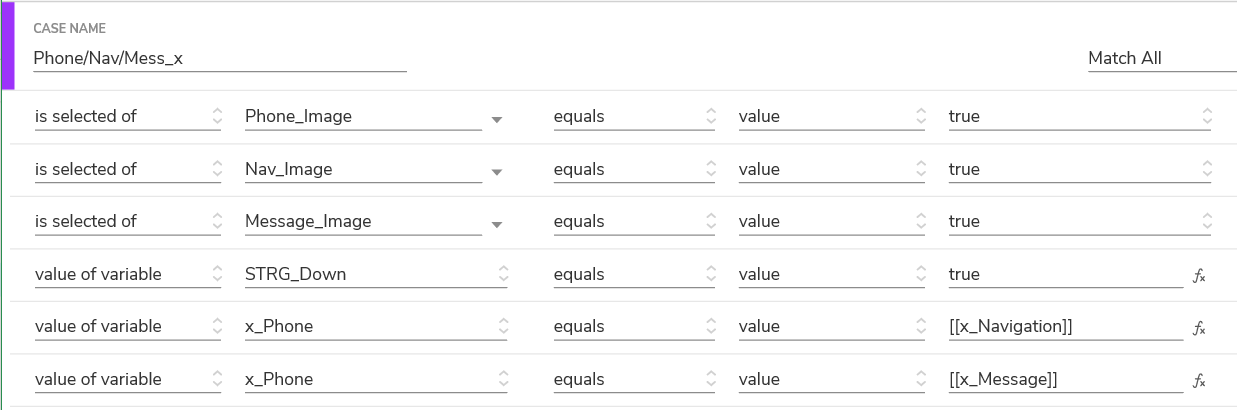
\includegraphics[scale=0.6]{figures/Prototyp_05.PNG}
  \captionof{figure}{Beispielbedingung Multiselektion}
  \label{fig:Prototyp_05}
\end{center}

Auf identische Art und Weise wurde diese Funktionalität für die verfügbaren Labels umgesetzt.
Aufgrund der Performance des Prototyps und der Fehleranfälligkeit wurde auf diese Anpassung bei der gleichzeitigen Auswahl von Texten und Bildern verzichtet.
Es ist hier möglich die Properties anzupassen, es wird jedoch nicht verglichen, ob deren Variablen den gleichen Wert aufweisen, stattdessen wird immer ein Strich angezeigt.
In \cref{fig:Prototyp_05} ist die logische Bedingung für den Fall zu sehen, dass alle drei Bilder gleichzeitig ausgewählt sind und deren x-Koordinate jeweils identisch ist.

Zeitgleich mit den Properties werden bei der Mehrfachselektion die Alignment Actions angezeigt.
Hier wird im Prototypen die Umsetzung in Bezug auf den Testcase eingeschränkt.
Da ein Startscreen modelliert werden soll, reicht die Möglichkeit die Bilder Horizontal aneinander auszurichten, die Vertikale Ausrichtung ist von Texten an Bildern möglich.
In \cref{fig:Prototyp_06} ist die Umsetzung im Prototyp zu sehen, wobei Teil a) bei zwei ausgewählten Bildern und Teil b) bei der gleichzeitigen Auswahl von Bild und Label sichtbar ist.
Die Alignment Actions liegen bei der Auswahl von zwei Objekten des gleichen Typs unten, und bei der Auswahl von zwei unterschiedlichen oben.
Bei letzterem Fall kann eher davon ausgegangen werden, dass keine Properties gemeinsam angepasst werden müssen, sondern die zwei unterschiedlichen Objekte eher aneinander ausgerichtet werden sollen.
Die tatsächliche Ausrichtung wird durch Klick auf den Button ausgelöst, indem der eingegebene Abstand auf den Variablenwert des weiter links oder weiter oben liegenden Objektes aufaddiert wird und der globalen Variable des zweiten Items zugewiesen wird.
Dadurch verschiebt sich das zweite Objekt und der Abstand der zwei Objekte entspricht dem eingegebenem Wert.

\begin{figure}%
\centering
\subfloat[][]{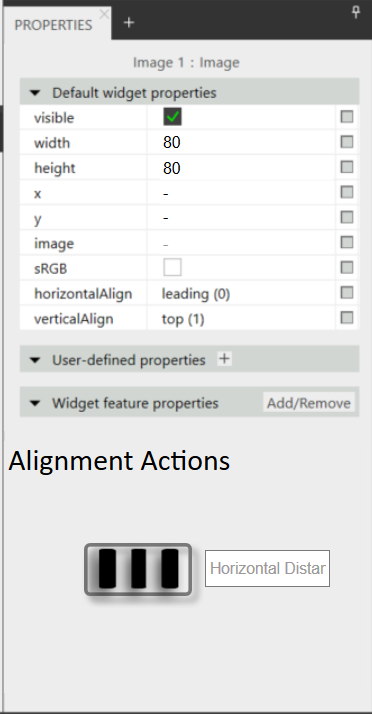
\includegraphics[width=0.3\linewidth]{figures/Prototyp_06.PNG}}%
\qquad
\subfloat[][]{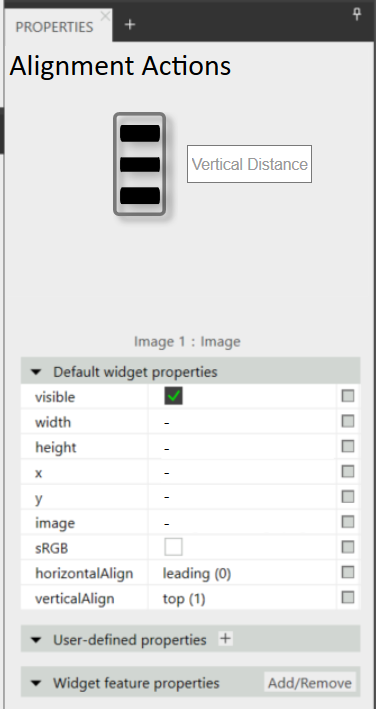
\includegraphics[width=0.3\linewidth]{figures/Prototyp_07.PNG}}%

\caption{Alignment Actions}%
\label{fig:Prototyp_06}
\end{figure}

\paragraph{Templates}
Das Anlegen von Templates wird ebenfalls mit Screenshots simuliert die mit Hotspots versehen werden.
Zusätzlich besteht hier noch die Notwendigkeit einen Imagetab neben dem View anzulegen, da das Erstellen der Templates in einer anderen View stattfindet.
In diesem Tab existiert ebenfalls ein Property Panel, die Funktion \glqq publish to template interface\grqq{} geschieht wie geplant über einen Klick auf den Kreis, der sich nach der Auswahl blau einfärbt.
Wird hier ein Wert angepasst wirkt sich das über eine globale Variable auch auf das Template Interface aus.
Eine Änderung im Template Interface darf jedoch nie ein Property des Templates anpassen.
Deshalb wurden hier zwei getrennte Sets von globalen Variablen angelegt, welche nur in eine Richtung synchronisieren.

\begin{center}
  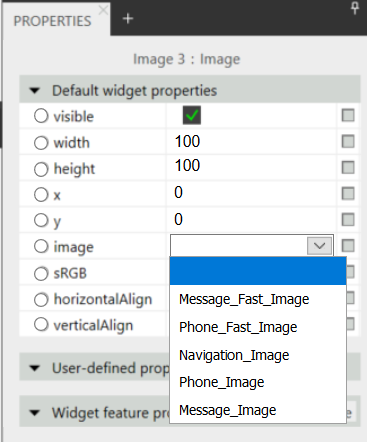
\includegraphics[scale=0.6]{figures/Prototyp_08.PNG}
  \captionof{figure}{Droplist für Images}
  \label{fig:Prototyp_08}
\end{center}

Die Zuweisung der Bilder im Template findet über ein Droplist statt, welche in \cref{fig:Prototyp_08} zu sehen ist.
Die Vorgehensweise, wie der sichtbare Inhalt eines Dynamic Panels mithilfe einer Droplist angepasst werden kann, wurde bereits in Abschnitt 4.1.1 erklärt.
Statt der bunten Kreise befindet sich in diesem Fall jeweils eine Ausführung aller Bilder in den Dynamic Panels welche je nach Auswahl aus der Droplist sichtbar oder unsichtbar geschaltet werden können.
Die alternative Vorgehensweise \glqq Insert in Template\grqq{} funktioniert nach dem selben Prinzip.
Nur wird hier nicht aus der Droplist abgefragt, sondern welches Bild aktuell im Template ausgewählt ist.
Dieses wird dann, nach einem Klick auf den Button entsprechend angezeigt.


\section {Implementierung Filter}
Nach Fertigstellung des Prototyps ist es nun nötig den Filter zu implementieren.
Da hier eine direkte Umsetzung im Sourcecode von EB GUIDE geplant ist, gibt es im Folgenden, nach der Formulierung der Zielsetzung,  einen groben Überblick über den Aufbau des Projektes.
Wie bei der Erstellung des Prototypen im vorherigen Kapitel wird abschließend noch aufgezeigt mit welchem Vorgehen die formulierten Ziele umgesetzt werden.

\subsection {Zielsetzung}
Das Ziel dieses Arbeitsabschnittes ist die Umsetzung des in Abschnitt 3.1.3 definierten optischen und funktionalen Designs.
Da es sich um eine Implementierung handelt ist hier keine Einarbeitung in ein Tool wie AXURE RP notwendig, vielmehr muss der Aufbau des bereits bestehenden Projektes verstanden werden.
Konkret muss für die Umsetzung des Designs eine Filterfunktion implementiert werden, die die bereits vorhandenen Widget Feature Properties nach den Wünschen des Nutzers filtert.
Hierfür wird für den Nutzer eine Eingabemöglichkeit benötigt, mit der er interagieren kann, wie er es von den Filterfunktionen anderer Anwendungen gewohnt ist.
Zusätzlich sollen bei der Nutzereingabe die aktuell bestehenden Kategorien verschwinden und in Echtzeit nur die passenden Features ohne zugehörige Kategorie angezeigt werden.

\subsection {Projektaufbau}

\paragraph{Programmiersprachen und Entwicklungsumgebung}
EB GUIDE Studio wird als WPF Anwendung umgesetzt und ist somit in C\# geschrieben.
WPF ist Teil des .NET-Frameworks 3.0, auf dessen Basis dem Entwickler eine große objektorientierte Klassenbibliothek zur Verfügung steht.
Innerhalb dieser Klassenbibliothek ist auch C\# zu finden, welche eine typsichere, objektorientierte Allzweck-Programmiersprache ist.
Für die Deklaration der Elemente des User Interfaces benutzt WPF die Beschreibungssprache XAML, welche auf XML basiert.

Da das Projekt firmenintern als eine Visual Studio Solution vorliegt, werden auch sämtliche Implementierungen im Rahmen dieser Arbeit innerhalb dieser Entwicklungsumgebung umgesetzt.

\paragraph{Design Pattern}
In der Projektentwicklung wird das Model-View-ViewModel (MVVM) Design Pattern angewandt.
Bei früheren Entwicklungen von User Interfaces, haben Entwickler häufig eine grafische View erstellt und im Nachhinein die Logik hinzugefügt.
Dies geschieht meist in Form von Eventhandlern, Initialisierungen oder Datenmodellen im Code Behind, was zu einer starken gegenseitigen Abhängigkeit von Interface und der dahinter liegenden Logik führt.
Dadurch entstehen Problematiken wie die Tatsache, dass nicht mehrere Entwickler gleichzeitig an der gleichen View arbeiten können, oder gegenseitig Code unbrauchbar gemacht wird.
Logik und Aussehen eines Interface an einer Stelle zu bündeln führt also zu schlechter Wartbarkeit, Erweiterbarkeit und ist kaum testbar\cite{.g}.
Die aufgeführten Probleme entstehen durch die starke Abhängigkeit der folgenden Komponenten.

\begin{itemize}
 	\item View (User Interface)
 	\item Model (Im User Interface angezeigte Daten)
	\item Zusammenfügender Code (Eventhandling, Abhängigkeiten, Logik)
\end{itemize}

Innerhalb des MVVM Pattern wird dieser zusammenfügende Code als das View Model bezeichnet.
Dessen grundlegende Aufgabe ist es, eine Trennung der View und des Models zu arrangieren und dadurch die Erstellung der Struktur und die Wartung der Anwendung zu vereinfachen.
Sobald sich ein Wert innerhalb des View Models ändert, wird die Anpassung, mithilfe von Data Binding und Benachrichtigungen, automatisch im View aktualisiert.
Wenn der Nutzer hingegen mit dem View interagiert, zum Beispiel einen Button drückt, wird eine, sich im View Model befindende Command ausgelöst, die die gewollte Aktion ausführt.
Während dieses Prozesses modifiziert das View Model die Daten des Models, die View selbst führt nie eine direkte Änderung auf dem Model aus.
Tatsächlich weiß die View nicht von der Existenz der Model Klasse, während das Model nicht weiß das die View existiert.

Das Pattern umfasst also die drei Hauptbestandteile:
\begin{itemize}
 	\item View (User Interface)
 	\item Model (Datenzugriffe, Modelklassen)
	\item ViewModel (Vermittler zwischen View und Model)
\end{itemize}

Wie in \cref{fig:MVVM} zu sehen, fungiert das ViewModel als Schnittstelle zwischen dem Model und der View. Es stellt ein Data Binding zwischen den beiden Instanzen bereit und verarbeitet über Commands alle Eingaben des Nutzers.
Die View bindet ihre Kontrollwerte an Properties des ViewModels, welche im Gegenzug die Daten der Modelobjekte bereit stellen.

\begin{center}
  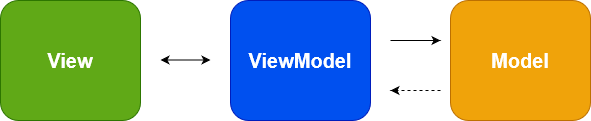
\includegraphics[scale=0.6]{figures/MVVM.PNG}
  \captionof{figure}{Model-View-ViewModel (MVVM) Design Pattern}
  \label{fig:MVVM}
\end{center}

Im aktuellen Projekt werden alle benötigten Models, meist in Form von Interfaces, in die ViewModel Klasse WidgetFeaturesOverlayViewModel importiert.
Aufgrund des Datenschutzes ist es nicht möglich, die genauen Models und die vollständige Implementierung der Klassen in dieser Arbeit offenzulegen.
Die in den folgenden Kapiteln erläuterten Ergänzungen, werden in die soeben erwähnte ViewMode Klassen und der dazugehörigen View WidgetFeaturesOverlayViewModel.xaml eingearbeitet.

\paragraph{CollectionViewSource}
Die zu filternden Elemente liegen innerhalb des Projektes bereits in Form einer CollectionViewSource vor.
Diese besitzt die Eigenschaften View und Source, welche jeweils unterschiedliche Varianten einer Collection beinhalten können.
Die View kann man hier als eine, über der Source liegenden Ebene verstehen, mit deren Hilfe die Darstellung der Collection manipuliert werden kann.
Das geschieht beispielsweise durch sortieren, filtern und gruppieren von Elementen, ohne jedoch die darunter liegende Source an sich zu verändern.
Falls die Source das Interface INotifyCollectionChanged implementiert, werden alle Änderungen, die durch das CollectionChanged event entstehen, an die View weitergeleitet.\cite{dotnetbot.}

Im konkreten Fall des vorliegenden Projektes besteht die Source aus einer ObservableCollection, welche die Feature Models des aktuell ausgewählten Widgets beinhaltet.
Eine ObservableCollection ist eine Collection dynamischer Daten, welche Benachrichtigungen für das Hinzufügen, Entfernen, oder Neuladen der Liste bereit stellt.
\cite{dotnetbot.c}
Aktuell wird die CollectionViewSource gruppiert und sortiert, wodurch die Einteilung in Kategorien und die alphabetische Sortierung in der View erzeugt wird.

\subsection {Vorgehensweise}
Zusätzlich zur Gruppierung und Sortierung stellt die CollectionViewSource ein Filter Event bereit.
Diese Filter können mithilfe der View auf die Collection angewendet werden. 
Das bedeutet konkret, dass ein Item zwar in der Collection Source existiert, mithilfe des Filterevents jedoch nur ein ausgewählter Teil dieser Collection in der View angezeigt wird.\cite{dotnetbot.b}
Das Event kann durch Setzen eines EventHandlers genutzt werden, welcher die gewünschte Filterlogik bereitstellen kann.
Dieser Eventhandler ist in Auflistung \ref{lst:CollectionViewSource}, in den Zeilen 22 bis 23 zu sehen, die dazugehörige Filterlogik in Auflistung \ref{lst:Filter}.

\newpage
\lstinputlisting[caption={CollectionViewSource()},captionpos=b, label=lst:CollectionViewSource]{listings/ICollectionView.cs}

Innerhalb der Filterfunktion muss zuerst abgefragt werden, ob der Filtertext leer ist oder Text beinhaltet.
Falls dies der Fall ist, ist es nicht nötig die Features zu filtern, weshalb alle verfügbaren mithilfe von Accepted zurückgegeben werden.
Sollte der Filtertext jedoch initialisiert worden sein, wird jedes Item innerhalb des Events als FeatureViewModel gespeichert.
FeatureViewModels enthalten alle relevanten Informationen über die Features.
Dazu zählt auch deren Namen, weshalb an dieser Stelle überprüft werden kann, ob die Eingabe des Nutzers einem Featurenamen entspricht oder in diesem enthalten ist.
Sollte dies der Fall sein, wird das Feature der gefilterten View hinzugefügt, anderenfalls wird das Feature durch den Filter entfernt.

\lstinputlisting[caption={Widget Properties Filter},captionpos=b,  label=lst:Filter]{listings/Filter.cs}

Die Grundstruktur des in Auflistung \ref{lst:CollectionViewSource} zu sehenden ICollectionView war im Projekt bereits vorhanden. 
Zusätzlich zu dem eben erwähnten Filter ist noch die If Abfrage in Zeile 9 ergänzt worden.
Diese dient dazu die ausklappbaren Kategorien auszublenden, sobald ein Filterbegriff eingegeben wird.
Die zweite Bedingung der If Abfrage in den Zeilen 5 und 6 ist ebenfalls neu hinzugefügt worden, um die Filterung in Echtzeit zu ermöglichen.
Bis jetzt war der erste Teil der Abfrage ausreichend, da die Liste nur einmal bei der Anzeige des entsprechenden Panels aktualisiert und angelegt werden musste, nach der Implementierung der Filterfunktion ist dies jedoch bei jeder Änderung des Filterbegriffes notwendig.
Aus diesem Grund wird nun auch abgefragt ob der Filtertext aktuell Text enthält, damit bei jedem ChangeEvent die Liste neu gefiltert wird.

Ausgelöst wird dieses ChangeEvent über den in Auflistung \ref{lst:Properties} zu sehenden Setter des Filtertextes.
Sobald eine Änderung im Textfeld registriert wird, schickt die View ein Update an das ViewModel, wodurch der Filtertext angepasst wird.
Zusätzlich dazu wird dem AvailableWidgetFeatures in Auflistung \ref{lst:CollectionViewSource} über das OnPropertyChanged Event mitgeteilt, dass die View aktualisiert werden muss.


\lstinputlisting[caption={Filtertext Properties},captionpos=b,  label=lst:Properties]{listings/Filter_Properties.cs}

Das Update vonseiten der View wird aufgrund des, in Auflistung \ref{lst:XAML} in Zeile 5 bis 6 zu sehenden, UpdateSourceTriggers ausgelöst. 
Hier wird über die Angabe des Paths festgelegt, dass bei jeder Änderung der Text Property die Properties des FilterTextes aktualisiert werden.
Zusätzlich wird hier ein Delay von 100 ms eingeführt, um die Filterung in Echtzeit zu ermöglichen.
Dieses Zeitintervall führt dazu, dass der Nutzer auch bei einer schnellen Eingabe nicht durch eine verzögerte Aktualisierung in seinem Arbeitsablauf unterbrochen  oder verlangsamt wird.

\lstinputlisting[caption={Filterpanel in xaml},captionpos=b,  label=lst:XAML]{listings/Filter_Panel.xaml}



\chapter{Usability Test}\label{ch:outlook}

Aufbauend auf allen bisher getätigten Analysen und Anpassungen des Interface, gilt es abschließend noch den Prototypen und die Implementierung mithilfe eines Usability Tests zu evaluieren.
Hierbei wird im Schritt \glqq Finalize the UX design\grqq{} des Human-Centered Design Process die Rolle des Usability Testers abgedeckt, welcher für die Durchführung der Auswertung des Usability Tests zuständig ist.
Auf weitere Anpassungen des Interface wird verzichtet.

In diesem abschließenden Kapitel werden die Grundlagen des verwendeten Tools für den Usability Test erläutert.
Darauf folgend wird die Art des durchgeführten Tests definiert und dargelegt auf welchen Grundlagen diese Wahl getätigt wurde.
Aufbauend auf den theoretischen Erläuterungen wird die letztendliche Testaufgabe konkret definiert und die nötigen Anweisungen, sowie die Materialien zur Auswertung der Tests erstellt.
Abschließend werden die Ergebnisse der durchgeführten Auswertungen der Tests dargestellt und interpretiert, bevor es einen Ausblick auf das mögliche weitere Vorgehen gibt.

\section{Lookback}

Bei Lookback handelt es sich um eine Cloudbasierte Softwarelösung, die es ermöglicht User Experience geräteübergreifend zu dokumentieren.
Bei der Durchführung der Tests besteht die Möglichkeit, als Tester aktiv teilzunehmen oder die Probanden unmoderiert mit dem Prototyp oder der Software interagieren zu lassen.
Möchte der Usability Tester teilnehmen -  also einen \glqq In Person\grqq{} Test durchführen - kann aus den beiden Möglichkeiten gewählt werden, die Tests mit dem Nutzer innerhalb einer Live-Session oder persönlich vor Ort an einem Rechner abzuhalten.

Für die durchzuführenden Tests erstellt der Usability Tester innerhalb von Looback ein Projekt.
Zugunsten des Datenschutzes besteht hier die Möglichkeit die Projekte auf privat zu setzen und nur ausgewählten Personen des Teams Zugriff zu den Aufnahmen  der Tests zu gewähren.
Innerhalb der Projekteinstellungen können Instruktionen für die Nutzer bereitgestellt werden, die während des Tests erscheinen und durch die Aufgaben führen.
Das ist vor allem dann hilfreich, wenn die Testperson den Test autonom durchführen soll.

Sollte der Test nicht gemeinsam in einem Raum stattfinden, kann mithilfe eines Links der Test mit den Probanden geteilt werden.
Der Tester bekommt eine Benachrichtigung, sobald der Proband bereit ist bzw. mit der autonomen Durchführung begonnen hat.
Während der Session hat der Tester die Möglichkeit mit Zeitstempel versehene Notizen zu machen oder mit eventuell teilnehmenden Teamkollegen zu chatten.
Diese Möglichkeit der Livedokumentation erleichtert die darauffolgende Auswertung des Test erheblich, da man sofort Auffälligkeiten festhalten kann und diese in der Aufzeichnung leichter auffindbar sind.
Nach Abschluss des Tests speichert Looback die Aufnahme in der Cloud, wodurch diese für die nachträgliche Auswertung des Tests abrufbar bleibt. \cite{.10.01.2020}

Die Möglichkeit der Livedokumentation bildet das ausschlaggebende Argument für die Wahl des Tools, ebenfalls besteht die Möglichkeit in der hochgeladenen Aufnahme Kommentare hinzuzufügen, was die Auswertung sehr erleichtert.
Zusätzlich ist es wichtig den Test online durchführen zu können, da viele Modellierer nicht am Hauptstandort von EB beschäftigt sind, wodurch persönliches Testen nicht immer möglich ist.

\section{Remote Usability Test}
Die im vorherigen Kapitel bereits kurz benannten \glqq In Person\grqq{} Tests finden in der Regel in einem Usability Labor statt.
Dies bezeichnet einen abgeschlossenen Raum ohne Störungsquelle, der mit der benötigten Hard- und Software ausgestattet ist und in dem sich nur der Proband und der durchführende Tester aufhalten.

Bei einem Remote Usability Test wird die Arbeitsaufgabe nicht gemeinsam im Labor, sondern räumlich getrennt durchgeführt.
Hier lässt sich noch zwischen asynchronen und synchronen Tests unterscheiden.
Bei letzteren besteht, trotz der räumlichen Trennung, eine direkte Verbindung mithilfe von Webcam und Sprachübertragung, zwischen Tester und Proband.
Gleichzeitig dazu wird der Bildschirminhalt der Testperson übertragen, um es dem Tester zu ermöglichen dessen Interaktionen zu verfolgen und durch die Aufgaben führen zu können.
Durch diese direkte Verbindung ist es für den Tester ebenfalls möglich, während, oder unmittelbar nach dem Test, Fragen zu stellen.
Bei synchronen Tests besteht der Vorteil darin, mit geringem Aufwand örtlich weit verteilte Nutzer in den Test einbinden zu können.
Zusätzlich dazu findet der Test in der gewohnten Umgebung des Nutzers statt, es wird also keine unnatürliche Situation in einem Labor geschaffen, was die Nervosität der Nutzer eventuell steigern könnte.
Auch können die Probanden hier mit ihrer gewohnten Hard- und Software arbeiten, was vor allem für repräsentative Werte, die die Effizienz betreffen, von Vorteil ist.
Durch den Umstand der gewohnten Arbeitsumgebung entsteht jedoch in vielen Fällen auch ein technischer Zusatzaufwand aufseiten des Nutzers.
So kann beispielsweise ein Headset und eine Webcam benötigt, oder zusätzliche Software auf dem Arbeitsgerät installieren werden müssen.
Dies ist in einem Usability Labor nicht notwendig, da hier eine einmalige Einrichtung der benötigten Hard- und Software stattfindet, die exakt auf den geplanten Test ausgelegt ist.

Im Rahmen eines asynchronen Tests besteht zusätzlich zu der räumlichen, auch noch eine zeitliche Trennung von Proband und Tester.
Identisch zum synchronen Test werden hier Gesicht und Bildschirminhalt der Testperson aufgezeichnet, der Nutzer kann jedoch aufgrund der Unabhängigkeit den Test zu einer, ihm passenden Zeit durchführen.
Da er dadurch jedoch auch auf sich allein gestellt ist, empfiehlt es sich zusätzliche Kommentare und Fragebögen in den Test einzubauen, um die direkte Befragung und Hilfestellung des synchronen Tests zu ersetzen.
Hier besteht ebenfalls der Vorteil, dass mit geringem Aufwand, großräumig verteilte Nutzergruppen eingebunden werden können.
Zusätzlich können durch die vollautomatische Erfassung der Ergebnisse auch sehr große Nutzergruppen effizient evaluiert werden.
Allerdings entstehen durch die zeitliche Trennung die Nachteile, dass - abgesehen von der Aufnahme - keine Beobachtungsdaten existieren.
Es kann also beispielsweise nicht darum gebeten werden, etwas genauer zu erläutern oder einen anderen Lösungsweg zu testen.
Die wohl größte Problematik bildet jedoch die Tatsache, dass nicht auf unerwartete Handlungen des Nutzers reagiert werden kann, was vor allem, bei nur teilweise funktionalen Prototypen, fatal sein kann.
Versuchen die Probanden hier einen Lösungsweg einzuschlagen, der in der vorliegenden Softwareversion nicht implementiert ist und auch nicht bedachte wurde, erhält die Testperson eventuell keine Rückmeldung des Systems.
Dies kann ohne weitere Unterstützung durch den Tester zum Abbruch des Test führen, was zu Unzufriedenheit aufseiten des Testers und Nutzers führen kann.\cite{Sarodnick.2016}

Da Lookback jeden der eben erläuterten Tests unterstützt, wirkt sich das Tool nicht einschränkend aus und die Wahl kann aufgrund relevanter Gründe getroffen werden.
Aufgrund der Tatsache, dass innerhalb der Testaufgabe mit einem Prototyp interagiert werden muss, ist ein synchroner Test dem asynchronen vorzuziehen.
Da dieser nicht alle, in GUIDE zur Verfügung stehenden, Interaktionsmöglichkeiten simuliert und die Funktion \glqq publish to template interface\grqq{} verlagert wurde, ist es wahrscheinlich, dass die Probanden an gewissen Punkten Unterstützung benötigen.
Es ist ebenfalls zu erwarten, dass in Bezug auf die neuen Funktionen Fragen bei den Testpersonen auftauchen werden, die nicht in der Arbeitsaufgabe beantwortet werden können.
Andererseits wird auch der Tester einige Aktionen genauer hinterfragen oder herausfinden wollen, warum gewisse Aktionen nicht durchgeführt wurden.

Grundsätzlich ist ein Test im Usability Labor, aufgrund der Ungestörtheit, immer dem Remote Test vorzuziehen.
Zum einen erstreckt sich die Nutzergruppe für diese Arbeit über mehrere Firmenstandorte von Elektrobit, weshalb es nicht möglich ist den Test mit allen Probanden in einem Labor durchzuführen.
Zum anderen soll mithilfe der Tests überprüft werden, ob eine Effizienzsteigerung erzielt werden kann.
Die Ausstattung in den Laboren entspricht nie hundertprozentig der gewohnten Umgebung der Nutzer, weshalb hier auch verminderte Leistungen, aufgrund der fremden Hardware zu erwarten sind.
Es wäre möglich, die Tests mit einem Teil der Probanden im Labor und mit dem anderen Remote durchzuführen.
Um die Ergebnisse jedoch so gut vergleichbar wie möglich zu halten, werden alle Untersuchungen unter den gleichen Bedingungen, in einem Remote Test, durchgeführt.

\section{Arbeitsaufgaben}
Um in der abschließenden Arbeitsaufgabe alle Änderungen testen zu können, ist es nötig sich an den ursprünglich analysierten Benutzeranforderungen zu orientieren, auf deren Grundlage die Änderungen entworfen und der Prototyp gebaut wurde.
Daher werden zu den, in Kapitel 3.0.3. bereits formulierten, qualitativen Anforderungen nun die, im Rahmen eines Tests messbaren, quantitative Nutzeranforderungen, für die ausgewählten Anpassungen ergänzt.

\textbf{Quantitative Benutzeranforderung für Template Properties}\newline
\textbf{Messung der Effizienz:}
Nutzer, die die Funktion \glqq publish to template interface\grqq{} über einen Linksklick auf den Kreis ausführen, sollen messbar schneller sein, als Nutzer, die dies über einen Rechtsklick auf das Quadrat tun. \newline
\textbf{Messung der Fehlerrate:} 
Nutzer, die die Funktion \glqq publish to template interface\grqq{} über einen Linksklick auf den Kreis ausführen, sollen eine niedrigere Fehlerrate aufweisen, als Nutzer, die dies über einen Rechtsklick auf das Quadrat tun.

\textbf{Quantitative Benutzeranforderung für Widget Feature Properties} \newline
\textbf{Messung der Effizienz:}
Nutzer, die die Filterfunktion nutzen, sollen schneller ein gewünschtes Widget Feature Property finden, als Nutzer die diese händische suchen müssen. \newline
\textbf{Messung der Fehlerrate:}
Bei Nutzern, die die Filterfunktion nutzen, soll die Fehlerrate sich, bei der Suche nach dem gewünschten Widget Feature Property, auf 0 reduzieren.

\textbf{Quantitative Benutzeranforderung für Mehrfachselektion}\newline
\textbf{Messung der Effizienz:}
Nutzer, die mehrere Objekte gleichzeitig selektiert haben, sollen deren korrekte Positionierung  und Skalierung schneller abgeschlossen haben, als Nutzer die keine Mehrfachselektion benutzen.\newline
\textbf{Messung der Fehlerrate:}
Nutzer, die Objekte mithilfe der Mehrfachselektion skalieren oder positionieren, sollen diesen Vorgang mit einer geringeren Fehlerrate abschließen, als Nutzer die keine Mehrfachselektion nutzen.

Zusätzlich wird hier darauf geachtet, inwiefern die Ergänzungen genutzt werden, vor allem die neu eingeführten \glqq Alignment Actions\grqq{} und die Funktion \glqq Insert in Template\grqq{} und welche Verbesserungen hier noch einzubringen sind.

Aus den aufgeführten Benutzeranforderungen lassen sich wiederum Subtask ableiten, anhand deren überprüft werden kann welche Interaktionen, vonseiten des Nutzers, in welcher Zeitspanne abgeschlossen werden, an welcher Stelle Fehler auftreten und welche Möglichkeiten nicht genutzt werden.
Hierfür ist es notwendig, jede Interaktion in kleine Subtasks zu untergliedern, um die exakte Stelle feststellen zu können, an der die Interaktion mit dem Interface zu Fehlern führt.
Bei der Filterung der Feature Widget Properties kann dies eventuell schon daran scheitern, dass nicht in das Texteingabefeld geklickt wird, oder erst durch die Eingabe eines falschen Filterbegriffes.
Die formulierten Subtasks für den in dieser Arbeit durchgeführten Test, lassen sich in Anhang \ref{app:Subtasks} nachvollziehen.

\begin{center}
  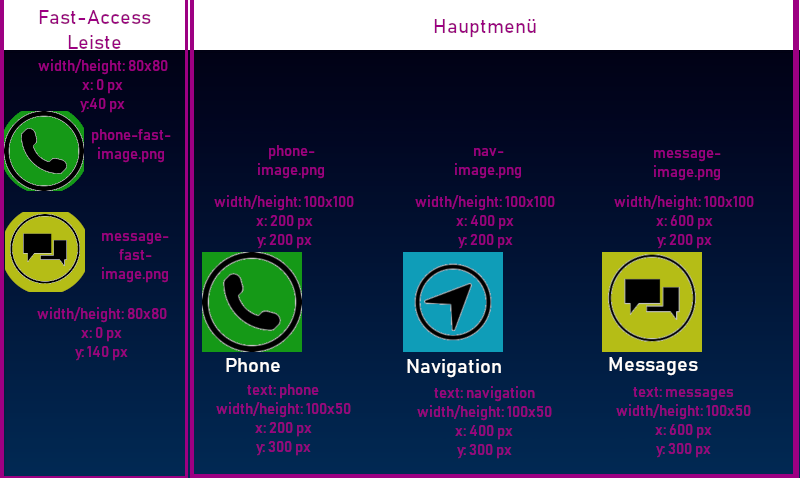
\includegraphics[width=0.9\linewidth]{figures/Styleguide_Rahmen.png}
  \captionof{figure}{Styleguide}
  \label{fig:Styleguide}
\end{center}

Auf Grundlage dieser Subtasks, scheint es weiterhin sinnvoll, den Testpersonen die Modellierung einen Startscreens eines Human Machine Interface der Automobilbranche als Testaufgabe modellieren zu lassen.
Hierfür ist es notwendig einen grafischen Styleguide zu erstellen an dem sich die Nutzer, wie aus ihrer täglichen Arbeit gewohnt, orientieren können.
Darüber hinaus ist es auch, für die Evaluierung der Tests, notwendig die Nutzer die exakt gleichen Aufgaben durchführen zu lassen.
Der, in \cref{fig:Styleguide} zu sehende, Styleguide zeigt einen Startscreen mit drei Bildern und Bildunterschriften im Hauptmenü und zwei Bildern in der Fast-Access-Leiste.
Für jedes dieser Elemente sind, die für den Modellierer relevanten Eigenschaften sichtbar, sowie die Namen der Bilder, wie sie auch in den Assets von EB GUIDE verwendet werden.
Diese Anmerkungen sind, innerhalb des Styleguides, alle in pink gehalten, um sie deutlich vom tatsächlichen Design abzugrenzen.
Wobei die Rahmen für das Hauptmenü und die Fast-Access Leiste ebenfalls der Orientierung dienen und zum Verständnis der, im Folgenden beschriebenen Arbeitsaufgabe notwendig sind.

Zusätzliche zu dieser grafischen Darstellung der Arbeitsaufgabe, wird noch eine textuelle Angabe erstellt, die für die Durchführung des Tests nötig ist.
Es werden insgesamt drei verschiedene Angaben erstellt, die in den Anhängen \ref{app:Aufgabe_Filter}, \ref{app:Aufgabe_Prototyp} und \ref{app:Aufgabe_Guide} zu finden sind.
Da ein Teil der Anpassungen implementiert und der andere Teil mithilfe eines Prototyps umgesetzt wurde ist es nötig den Test in zwei Teile aufzuspalten, weshalb auch zwei getrennte Angaben existieren.
In Testaufgabe \ref{app:Aufgabe_Filter} gilt es den implementierten Filter zu testen, weshalb die Nutzer hier aufgefordert werden, die drei Bilder für das Hauptmenü zu platzieren und mit Widget Feature Properties zu versehen.
Für diesen ersten Teil wird den Nutzern ein vorbereitetes Projekt mit den benötigten Assets zur Verfügung gestellt, um zu gewährleisten, dass Probanden mit einer identischen Ausgangssituation starten.
Es wird hier explizit nicht auf die implementierten Änderungen hingewiesen, da überprüft werden soll, ob diese von den Nutzern intuitiv benutzt wird.
Um jedoch zu gewährleisten, dass jeder Nutzer das Filterfeld theoretisch nutzen kann, wird darum geben die Bilder mit Widget Feature Properties zu versehen.

Für Aufgabe \ref{app:Aufgabe_Prototyp} ist es notwendig den Übergang in den Prototyp so nahtlos wie möglich zu gestalten und gleichzeitig wieder eine identische Ausgangssituation für alle Nutzer zu schaffen.
Das initiale Aussehen des Prototyps beinhaltet deshalb die drei eingefügten Bilder im Hauptmenü, entspricht also der Situation, mit der das vorherige Projekt in GUIDE von den Testpersonen verlassen wurde.
Da die Multiselektion eine Neuerung ist, die eher unwahrscheinlich selbstständig von den Nutzern entdeckt wird, wird hier zu Anfang darauf hingewiesen, dass der vorliegende Prototyp Multiselektion unterstützt.
Mit der Fast-Access Leiste, welche mithilfe von Templates modelliert werden soll, wird die Verlagerung der Funktion \glqq publish to template interface\grqq{} überprüft.
Ebenfalls wird in diesem Zuge darauf hingewiesen, dass nun auch Bilder mithilfe von Multiselektion in Templates eingefügt werden können, jedoch ohne genaue Erklärung, auf welche Art und Weise das funktioniert.
Abschließend sollen noch die Bilder und Labels positioniert und skaliert werden.
Es wird hier nicht mehr explizit auf die Multiselektion verwiesen, da herausgefunden werden soll, inwiefern die Probanden dies, nach der Information zu Beginn der Angabe, intuitiv für die restliche Aufgabe nutzen.

Die letzte Aufgabe \ref{app:Aufgabe_Guide} dient zur Erlangung der Vergleichswerte der Effizienz und wird deshalb in der unmodifizierten Version von GUIDE umgesetzt.
Da hier kein Übergang in den Prototyp notwendig ist, ist eine zusammenhängende Arbeitsaufgabe ausreichend.
Die Probanden sollen hier die identische Aufgabe durchführen und werden, angepasst an die beiden vorherigen Angaben, in der Nutzung von Templates eingeschränkt oder dazu aufgefordert.
Den Nutzern hier ein komplett freies Arbeiten zu gestatten ist nicht möglich, da möglichst identische Arbeitsschritte getätigt werden müssen um einen validen Vergleich anstellen zu können.

\section {Ergebnisse}
Die Anzahl der - in einem mit n Nutzern durchgeführten Test -  gefundenen Usabilityprobleme lässt sich laut Nielsen und Landauer nach folgender Formel berechnen.

\begin{center}
$\mathbf{N (1-(1- L ) ^n )}$ 
\end{center}

Wobei N der kompletten Anzahl der Usabilityprobleme im System entspricht und L der Anzahl der entdeckten Probleme nach dem Test mit einem Nutzer.
L entspricht hier im Durchschnitt 31\%, was zu der folgenden Grafik führt.  \cite{Nielsen.1993}

\begin{center}
  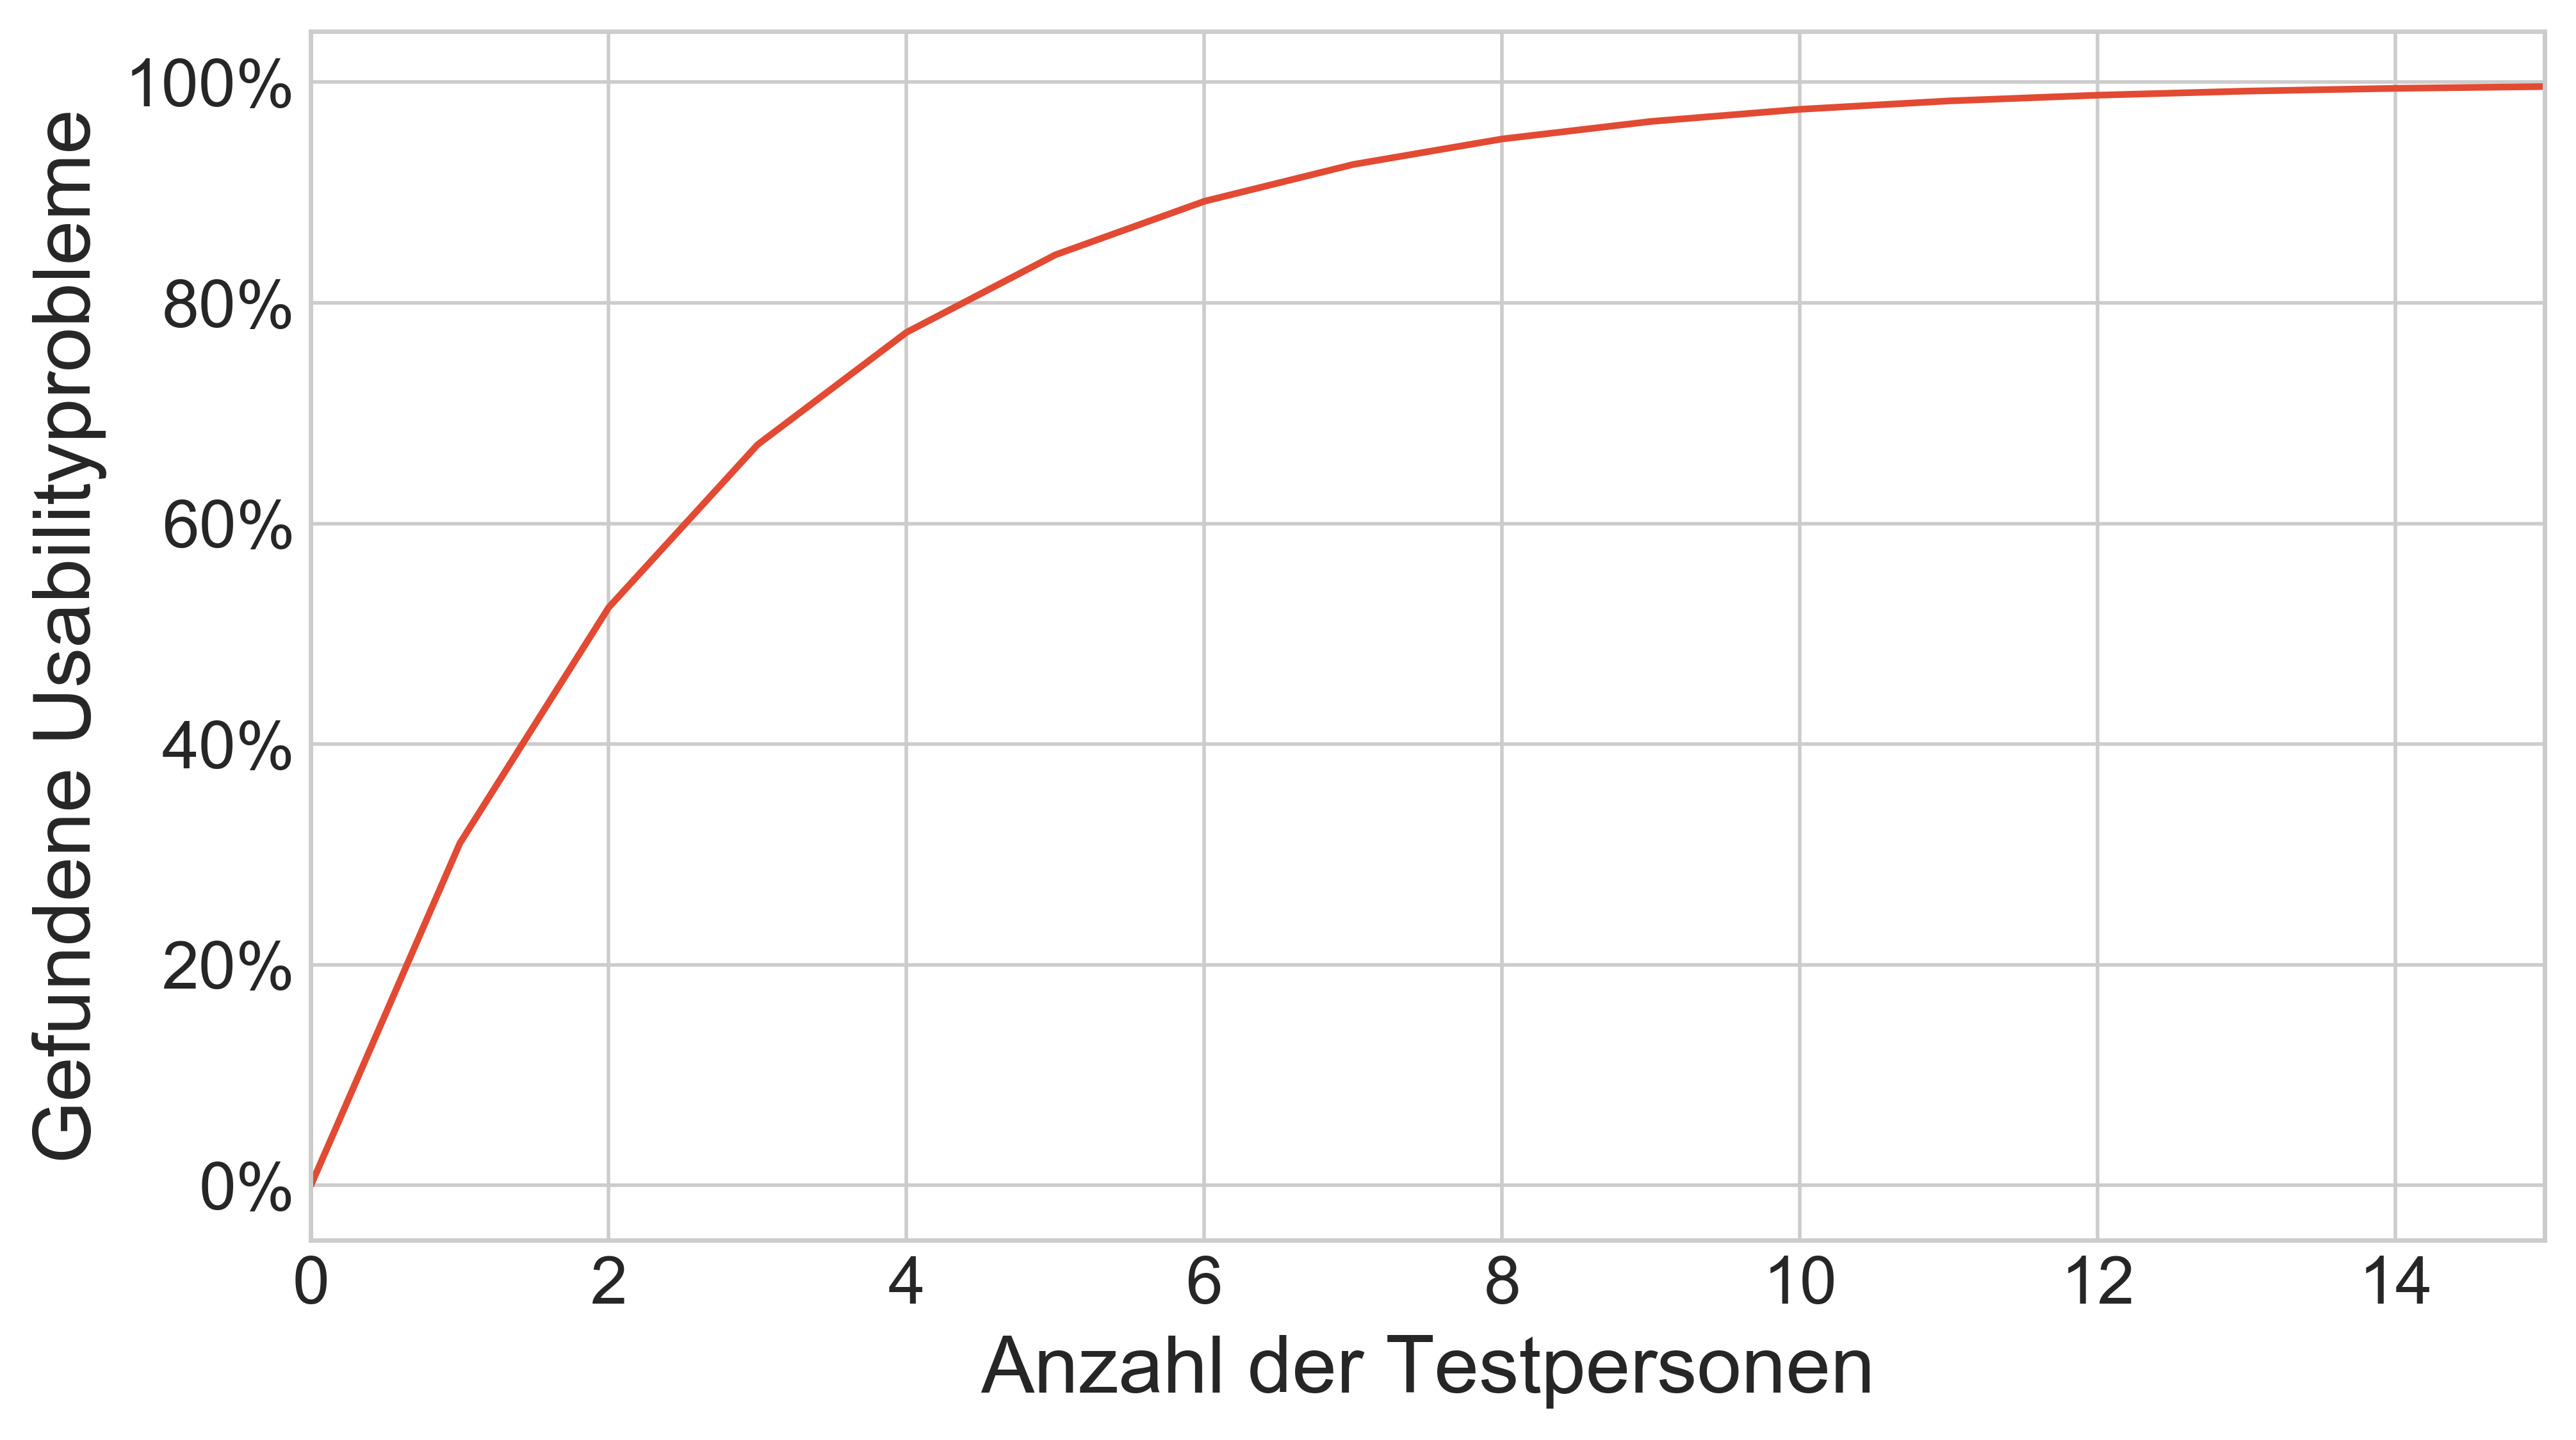
\includegraphics[width=0.7\linewidth]{figures/curve.png}
  \captionof{figure}{Aufdeckungsrate von Usabilityproblemen}
  \label{fig:curve}
\end{center}

Bei Betrachtung von \cref{fig:curve} wird deutlich, dass - solange mit keinem Nutzer getestet wurde - es auch keinen Aufschluss über die Usability Probleme eines Systems gibt.
Nach dem Test mit einem Nutzer, werden bereits fast ein Drittel der Schwächen aufgedeckt.
Wird der Test mit einem zweiten Nutzer durchgeführt, decken sich bereits einige der Beobachtungen, es werden aber durchaus noch neue Schwächen entdeckt und unterschiedliche Messergebnisse treten auf.
Je mehr Nutzer untersucht werden, desto häufiger decken sich die Beobachtungen und Messungen mit den Ergebnissen der bereits untersuchten Nutzer.\cite{.h}
Entgegen einer häufigen Annahme ist es also nicht unbedingt sinnvoll einen Usability Test mit einer möglichst großen Zahl an Testpersonen durchzuführen, da der Tester, ab einem gewissen Punkt, fast ausschließlich identische Probleme sehen und Messwerte erhalten wird.
Neue Informationen erhält man meist bis zur Untersuchung des fünften Nutzers, weshalb dies auch die optimale Anzahl an Probanden darstellt.

Wird nun aber, wie im Falle dieser Arbeit, eines der messbaren Usability Attribute verglichen, ist es nötig die Anzahl der Nutzer zu verdoppeln.
Es werden zwei verschiedene Versionen eines Systems verglichen, die jeweils von fünf Nutzer getestet werden.
Dadurch werden bei jedem System etwa 80\% bis 90\% der Schwächen aufgedeckt.
Bei der Messung der Attribute Effizienz und Fehlerrate kann ein repräsentativer Mittelwert gebildet werden.

Alternativ gäbe es die Möglichkeit den Test mit nur fünf Nutzern durchzuführen, was zu dem Vorteil führen würde, die Ergebnisse einer Person mit dem neuen und alten Interface direkt vergleichen zu können.
Allerdings würde hier die Problematik entstehen, dass der Nutzer die gleiche Arbeitsaufgabe doppelt durchführen würde, was zu einer Verfälschung der Ergebnisse führt, da die Angaben und Koordinaten der Objekte bereits bekannt sind.
Die Durchführung der identischen Arbeitsaufgabe ist jedoch dringend notwendig, um vergleichbare Werte zu erhalten.
Aus diesem Grund bevorzugt Nielsen die Messung mit der doppelten Anzahl an Probanden, statt Nutzern zweimal die gleiche Aufgabe durchführen zu lassen.\cite{.h}

Die im Folgenden dargestellten Ergebnisse wurden durch das Testen einer Gruppe aus zehn Personen erzeugt, die aus sechs Expertennutzern und vier Gelegenheitsnutzern besteht.
Zwar wäre eine 1:1 Zusammensetzung der Gruppe der Testpersonen wünschenswerter, firmenintern standen jedoch zum Zeitpunkt der Messung nicht mehr Personen zur Verfügung, weshalb es einen Expertennutzer mehr in der Testgruppe gibt.
Die Einstufung eines Expertennutzers wird dadurch definiert, dass die Person aktuell aktiv in einem Projekt mit EB GUIDE 6 arbeitet und dies auch schon seit mindestens 2 Monaten ununterbrochen tut.
Gelegenheitsnutzer sind all diejenigen, die zwischen dem Nutzen der Software immer mindestens 2 Wochen pausieren und eine einführende Schulung erfolgreich abgeschlossen haben.

Aus den gemessenen Werten wird jeweils ein Mittelwert gebildet, zusätzlich wird bei den Neuerungen untersucht welcher der möglichen Wege zur Problemlösung genutzt wird und welcher nicht.
Über die Fehlerrate kann ergänzend aufgedeckt werden, ob noch Verbesserungen am Design vorgenommen werden müssen.

\subsection{Ergebnisse überarbeitetes Interface}
Der Prototyp und der implementierte Filter werden demnach mit fünf Probanden getestet, welche sich aus drei Experten und zwei Gelegenheitsnutzern zusammensetzen.
Nach der Durchführung der Aufgabe werden den Nutzern noch zusätzliche Fragen zu ihrem Verhalten gestellt, welche in der folgenden Auswertung ebenfalls aufgeführt werden.

\paragraph{Widget Feature Properties}
Der Filter wird im Test von drei Probanden genutzt, die anderen beiden, jeweils ein Experte und ein Gelegenheitsnutzer, geben anschließend an die Funktion nicht gesehen zu haben.
Ein Nutzer wendet den Filter erst an, nachdem er zwei Menüs auf der Suche nach dem richtigen Feature ausgeklappt hat.
Er und die anderen Beiden geben anschließend an, den Filter nicht als Neuerung wahrgenommen zu haben, ihn jedoch intuitiv genutzt zu haben.

Die Auswahl eines Feature Properties dauert mithilfe des Filters durchschnittlich 2 Sekunden.
Zwei der Nutzer erzeugen eine Fehlerrate von 2 Fehlern bei der Auswahl.
Aus der Suche nach dem Scale Mode filtern die Probanden mit dem Wort \glqq Scal\grqq{}.
Dadurch taucht, wie in \cref{fig:Feature_Test} zu sehen, in der Ergebnissen zusätzlich zu dem Scale Mode das Feature Scaling auf, welches dann fälschlicherweise ausgewählt wird.

\begin{center}
  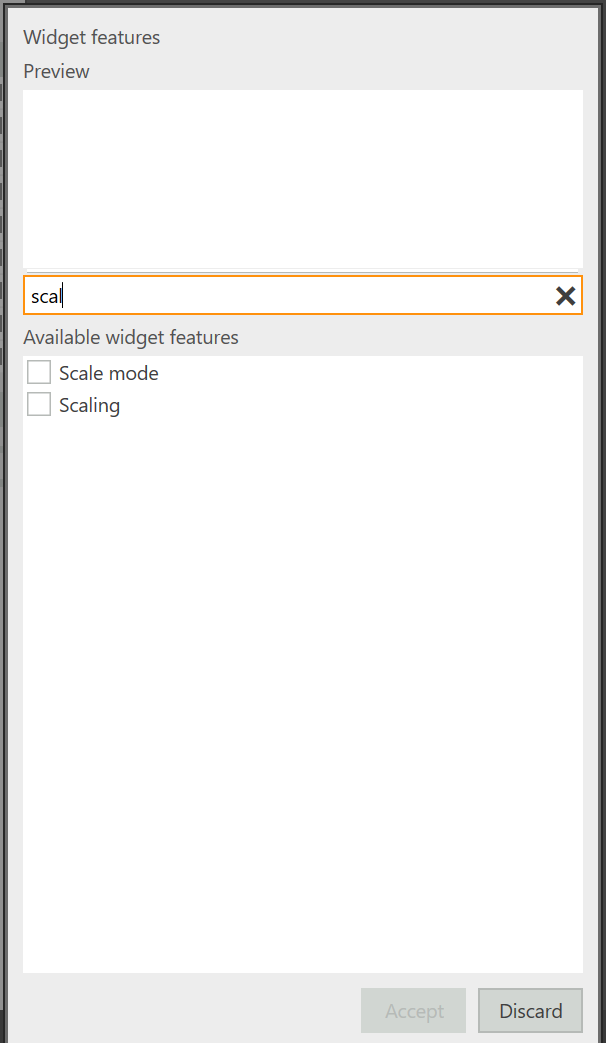
\includegraphics[scale= 0.6]{figures/Feature_Test.PNG}
  \captionof{figure}{Filterung nach Scale Mode}
  \label{fig:Feature_Test}
\end{center}

\paragraph{Publish to template interface}
Die Verlegung des Hotspots für die Funktion \glqq publish to template interface\grqq{} wird ebenfalls von drei, der fünf Probanden selbstständig gefunden, die alle benötigten Properties dadurch in durchschnittlich 4,6 sek publishen können.
Die neue Position wird von einem Experten und einem Gelegenheitsnutzer nicht entdeckt, jedoch - nach Aufklärung vonseiten des Testers - als nützlicher Shortcut eingestuft.
Bei den nötigen Klicks für die das Publishen der Objekteigenschaften wird eine Fehlerrate von 0 erzielt.

\paragraph{Multiselektion}
Für die Skalierung der drei Bilder des Hauptmenüs nutzen alle Probanden die Multiselektion und schließen den Vorgang in durchschnittlich 7,2 Sekunden ab, wobei ihnen keine Fehler unterlaufen.

Bei den Labels haben nur vier Testpersonen die Multiselektion in durchschnittlich 8 Sekunden mit einer Fehlerrate von 0 genutzt, der fünfte Nutzer hat, nach eigenen Aussagen, aus Gewohnheit jeden Text einzeln positioniert, obwohl vorher für die Bilder die Mehrfachselektion verwendet wurde.

Bei der Positionierung muss unterschieden werden, ob die Arbeitsaufgabe mithilfe der Alignment Actions oder mit einfacher Multiselektion gelöst wurde.

Ein Proband macht bei den Bildern Gebrauch von den Alignment Actions und schließt die Positionierung aller drei Bilder in 5 Sekunden ab.
Allerdings lässt sich hier eine Fehlerquelle beobachten.
Der Nutzer legt zuerst den Abstand zwischen den Objekten fest, vergisst jedoch das Ankerbild, an dem sich die anderen Bilder ausrichten, an die richtige Position zu setzen.
Nachdem dieses korrekt positioniert ist muss die Ausrichtung erneut durchgeführt werden.
Drei der anderen Nutzer haben die Alignment Actions bei den Bildern nicht gesehen, ein Vierter hat sie zwar wahrgenommen, hatte zu diesem Zeitpunkt die Bilder jedoch einzeln schon korrekt positioniert, dass er von der Nutzung abgesehen hat.

Bei den Labels nutzt dieser Proband die Alignment Actions, ebenso die Testperson, die diese Funktion auch bei den Bildern angewandt hat.
Dadurch kann die Positionierung hier in durchschnittlich 6 Sekunden abgeschlossen werden, es tritt jedoch ein identischer Fehler mit dem Ankerobjekt auf, was hier ebenfalls eine Fehlerrate von 1 ergibt.
Die Probanden die diese Funktion nicht nutzen, geben hierfür die gleichen Gründe an wie bei den Bildern.

Zusätzlich gibt es bei den Texten die Möglichkeit diese mithilfe der Alignment Actions an den Bildern auszurichten.
Auf die Idee ein Bild und den dazugehörigen Text gleichzeitig auszuwählen kommt jedoch keine der Testpersonen.
Dies ist darauf zurückzuführen, dass sich erst noch an die neuen Funktionen gewöhnt werden muss und die gleichzeitige Auswahl verschiedener Objekte zum aktuellen Zeitpunkt noch zu verwirrend ist.

Die Positionierung über normale Multiselektion wird bei den Bildern von vier Nutzern durchgeführt, wobei die identischen y-Koordinaten zusammen angepasst werden und danach die x-Koordinate für jedes Bild einzeln.
Mit diesem Vorgehen ist die Positionierung in durchschnittlich 3,5 Sekunden abgeschlossen und es werden zusätzlich keine Fehler gemessen.

Bei den Texten ist das Vorgehen für die Positionierung identisch, es treten ebenfalls keine Fehler auf und die durchschnittliche Zeitspanne beträgt 4,6 Sekunden.

Die Funktion \glqq Insert in Template\grqq{} wird von keinem der Nutzer entdeckt. Bei der abschließenden Befragung geben auch alle Probanden an, dass sie diese Funktion als nicht sinnvoll erachten.

\subsection{Ergebnisse altes Interface}
Um die Vergleichswerte zu erhalten wurde die Testaufgabe mit dem bestehenden Interface ebenfalls mit fünf Personen durchgeführt.
Die Zusammensetzung aus drei Experten und zwei Gelegenheitsnutzern ist hier identisch zu der Testgruppe des Prototypen.

\paragraph{Widget Feature Properties}
Da hier keine Filterfunktion zur Verfügung steht treten, wie zu erwarten, mehr Fehler bei den Nutzern auf.
Von den fünf Probanden begehen zwei Nutzer 2 Fehler und ein Nutzer 3 Fehler.
Die restlichen beiden Testpersonen finden das gewünschte Feature auf Anhieb, müssen hier jedoch einige Sekunden überlegen, weshalb bis zu Wahl des gewünschten Properties durchschnittlich 8,8 Sekunden vergehen.

\paragraph{Publish to template interface}
Die Funktion \glqq publish to template interface\grqq{} wird in der aktuellen Version von den Probanden in durchschnittlich 16 Sekunden abgeschlossen.
Eine Person erzeugt hier eine Fehlerrate von 1, indem sie nach dem Rechtsklick auf das Rechteck hinter dem zu verlinkenden Property zuerst die falsche Funktion auswählt.
Bei allen anderen Probanden lässt sich ebenfalls beobachten, dass sie kurz überlegen, welche der in \cref{fig:Template} zu sehenden Alternativen ausgewählt werden muss.
\begin{center}
  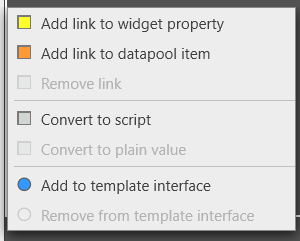
\includegraphics[scale= 0.8]{figures/Template.PNG}
  \captionof{figure}{Auswahlmöglichkeiten nach Rechtsklick auf Templateproperties }
  \label{fig:Template}
\end{center}

\paragraph{Positionieren/Skalieren ohne Multiselektion}
Das Skalieren und Positionieren der Texte und Bilder wird in der aktuellen Version von GUIDE  von den Nutzern meist so gelöst, dass ein Bild mit allen nötigen Features ausgestattet und dieses dann kopiert wird.
Anschließend ist es noch nötig die unterschiedlichen Eigenschaften der Kopien entsprechend der Spezifikation anzupassen.

Da bei der Skalierung die Werte nach dem Kopieren nicht mehr verändert werden müssen, kommen die Probanden hier auf eine durchschnittliche Arbeitszeit von 4,8 Sekunden, in der der Kopiervorgang bereits einberechnet ist.
Fehler treten hier nur auf, wenn die Probanden die Werte nicht händisch eingeben, sondern mit dem etwas komplizierteren Ansatz der Datapoolitems arbeiten.
Hierbei werden die Eigenschaften, wie Breite und Höhe mit einem Item verlinkt, dessen Wert sich an einer Stelle zentral anpassen lässt und alle verlinkten Objekte entsprechend verändert.
Fehler treten hierbei durch Verlinkung des falschen Datapoolitems oder der Eingabe des falschen Wertes auf.
Die Anzahl bemisst sich in diesem Testfall auf 2 Fehler bei einem Probanden, der diesen etwas komplizierteren Modellierungsansatz wählt.

Bei der Skalierung der Labels arbeitet keiner der Nutzer mit Datapoolitems, weshalb hier eine Fehlerrate von 0 erzeugt wird und der Vorgang für alle Texte in durchschnittlich 9 Sekunden abgeschlossen ist.

Für die Positionierung der Bilder und Labels müssen die Eigenschaften der kopierten Elemente angepasst werden.
Dies geschieht für erstere in 8,5 Sekunden, bei den Labels dauert es durchschnittlich 10,8 Sekunden.
Hierbei tritt bei den Bildern ebenfalls ein Fehler bei der Arbeit mit den Datapoolitems auf, bei den Texten beläuft sich die Fehlerrate bei allen Nutzern auf 0.

\subsection{Vergleich und Interpretation}Auf Grundlage der gemessenen Daten kann nun ein direkter Vergleich zwischen dem bestehenden und dem überarbeiteten Interface von EB GUIDE getätigt werden.
Weiterhin können Beobachtungen über die Nutzung der Ergänzungen interpretiert werden und anhand der Messwerte evaluiert werden, ob die definierten quantitativen Benutzeranforderungen erfüllt wurden.

\paragraph{Widget Feature Properties}
Mithilfe des Filters gelingt es den Probanden 8,8 Sekunden schneller das gewünschte Feature Property zu finden, wodurch die Anforderung an die Effizienz erfüllt ist.
Die angestrebte Fehlerrate von 0 kann jedoch aktuell noch nicht erzielt werden.
Die Fehler können sich vermutlich darauf zurückführen lassen, dass die Nutzer an die übergeordneten Kategorien gewöhnt sind und sich deshalb nicht sicher sind, ob sie Scaling oder Scale Mode auswählen müssen.
Hier bestünde die Möglichkeit in einer weiteren Iteration zu testen ob sich die Fehleranzahl wieder verringert, wenn die Kategorien während des Filterns eingeblendet bleiben.

\paragraph{Publish to template interface}
Die neue Position der Publish Funktion wurde zwar nicht von allen Nutzern selbstständig gefunden, wurde jedoch im Nachhinein von allen als sinnvoll eingestuft.
Die erreichte Fehlerrate von 0 stellt hier eine Verbesserung dar, da bei der jetzigen Implementierung teilweise falsche Optionen ausgewählt werden und die Nutzer lange überlegen müssen.
Zusätzlich schließen die Probanden ihr Vorgehen 11,4 Sekunden schneller ab, was sich auf den fehlenden Rechtsklick zurückführen lässt.
Damit sind beide Benutzeranforderungen für diese Funktion erfüllt.
Trotzdem kann die neue Position die vorherige nicht in Gänze ersetzen, da es für Erstnutzer nicht möglich ist, die Funktion des Klicks zu erkennen.
Daher bietet sich eine Kombination der bisherigen Implementierung und der Neuerung an.
Nutzer, die sich der Funktion bewusst sind, können den schnelleren Weg über Klick auf den Kreis wählen, Modellierer die sich noch mit der Funktionsweise von GUIDE vertraut machen, können die bisherige Variante mit dem erklärenden Text wählen.

\paragraph{Multiselektion}
Die Funktion \glqq Insert in Template\grqq{} wurde von keinem der Probanden benutzt und auch bei einer nachträglichen Befragung als nicht hilfreich eingestuft.
Deshalb erscheint es hier sinnvoll diese Funktion nicht weiterzuverfolgen.

Die Alignment Actions beschleunigen die Positionierung der Bilder und der Texte, bringen jedoch aktuell noch eine höhere Fehlerrate mit sich, als die bis jetzt übliche Art der Positionierung.
Die begangenen Fehler lassen sich jedoch auch darauf zurückführen, dass diese Funktion in GUIDE eine komplett neue und daher ungewohnte Ergänzung bietet.
Neue Funktionen müssen erst getestet und verstanden werden.
Die falsche Ausführungsreihenfolge ist ein Fehler, der vermutlich nur zu Anfang und nicht mehr bei regelmäßigem Gebrauch auftritt.
Diese Möglichkeiten zu erweitern und fortlaufend zu untersuchen würde sich also lohnen.
Auch das Alignment von Text an Bildern sollte, zumindest für eine weitere Iteration, weiter verfolgt werden, um herauszufinden, ob die Nutzer, da sie nun von dieser Funktionalität wissen, diese auch benutzen.
Die Anforderung der höheren Effizienz wird durch die Alignment Actions demnach bereits erfüllt, in Bezug auf die Fehlerrate sind jedoch noch Nachbesserungen erforderlich.

Die Positionierung der Elemente ohne Alignment Actions, sondern nur mit Multiselektion, hat innerhalb des durchgeführten Tests  mit 3,5 Sekunden zeitlich am besten abgeschnitten, auch wurden hier keine Fehler durch die Nutzer begangen.
Gleichzeitige Anpassung von Properties scheint sowohl zeitlich sinnvoll, als auch für den Nutzer intuitiv zu verlaufen und erfüllt zudem die formulierten Benutzeranforderungen.

Bei der Skalierung der Bilder bietet die Multiselektion, auf den ersten Blick, keinen zeitlichen Vorteil.
Es gilt jedoch zu bedenken, dass im Testfall nur drei Bilder vorhanden sind, der Kopiervorgang dieser Bilder also kein großes zeitliches Gewicht hat.
Beinhaltet eine Spezifikation jedoch beispielsweise zehn, statt nur drei Bilder, geht durch den Kopiervorgang bereits mehr Zeit verloren.
Den Ansatz, die Objekte zu kopieren und dann entsprechend anzupassen, haben die Nutzer nur bei den Bildern, jedoch nicht bei den Texten verfolgt.
Deshalb lässt sich bei den Messwerten innerhalb des Prototyps eine zeitliche Verbesserung gegenüber der bisherigen Version verzeichnen.
Da sich die Multiselektion für die Positionierung bereits als Mehrwert erwiesen hat, ist es sinnvoll die gleichzeitige Anpassung aller Properties bei Mehrfachselektion zu ermöglichen.
Es würde den Nutzer irritieren, wenn nur gewisse Eigenschaften gleichzeitig anpassbar wären, weshalb es sinnvoll ist, auch weiterhin width und height der Objekte zusammen anpassen zu können.
In weiteren Iteration wäre es hier jedoch sinnvoll zu untersuchen, ob bei größeren Projekten tatsächlich ein zeitlicher Mehrwert eintritt, da dies hier lediglich vermutet wird.
Die Benutzeranforderungen sind, im Bezug auf die Skalierung der Objekte, dementsprechend noch nicht komplett erfüllt.
Die Fehlerrate beläuft sich zwar weiterhin auf 0, allerdings ist ein Mehrwert im Bezug auf die Effizienz noch nicht sichergestellt.

\section {Ausblick}
Die vorliegenden Ergebnisse werden auf Grundlage einer Iteration des Human Centered Design Process erlangt.
Je nachdem, ob nach dieser Iteration die Benutzeranforderungen erfüllt sind, ist es notwendig das Design anzupassen und nochmals zu evaluieren oder es als abgeschlossen zu betrachten und zur Implementierung überzugehen.

Wie im vorherigen Abschnitt bereits festgehalten erfüllt die Filterfunktion noch nicht alle Anforderungen und bedarf in Bezug auf die Fehlerrate noch einer Nachbesserung.
Diese gilt es in einem weiteren Test erneut zu evaluieren.

Die neue Position der Funktion \glqq publish to template interface\grqq{} erfüllt alle definierten Bedingungen und kann deshalb, zusätzlich zur bestehenden Funktion, implementiert werden.

Die Funktionen der Multiselektion gilt es an diesem Punkt differenziert zu betrachten.
Da diese Ergänzung komplett neu in EB GUIDE sind, gibt es hier noch viele Möglichkeiten und Funktionen, die hinzugefügt und evaluiert werden können.
Das gleichzeitige Anpassen von Eigenschaften, wie der Position und Skalierung von Objekten, hat sich im Rahmen dieser Iteration bereits als nützlich erwiesen und kann ebenfalls implementiert werden, da herausgefunden wurde, dass die Modellierer diese Funktion auch nutzen.
Dadurch wird eine Grundlage für weitere Interaktionsmöglichkeiten dieser Art gelegt.
So ist es beispielsweise üblich die Eigenschaften, die nun gemeinsam anpassbar sind, mit Datapoolitems zu verlinken.
Bei den Befragungen nach dem Tests äußern hier einige der Nutzer den Wunsch diese Verlinkung ebenfalls, mithilfe der Multiselektion durchführen zu können, was für eine weitere Iteration im Prototyp ergänzt und evaluiert werden kann.
Zusätzlich wird angegeben, dass über dem Propertie Panel angezeigt werden soll, welche Objekte aktuell zusammen ausgewählt sind, da dies bis jetzt nur im View erkennbar ist.

Da bei den durchgeführten Tests deutlich wird, dass die Nutzer sich für die Alignment Actions interessieren, kann nun in folgenden Iterationen noch eine Verbesserung und Erweiterung der Funktionalitäten angestrebt werden.
Für diesen Test war der Prototyp so ausgelegt, dass bereits bekannt war, welches der drei Bilder des Hauptmenüs links, rechts und in der Mitte liegt.
Dadurch hat sich die Anordnung, durch einen Klick auf den Button, automatisch an die Spezifikation angepasst.
Für tatsächliche Arbeitsabläufe ist dies nicht der Fall, weshalb es für den Nutzer möglich sein muss, anzugeben in welcher Anordnung die Bilder platziert werden sollen.
Dies wäre zum Beispiel dadurch umsetzbar, dass der Nutzer ein Objekt als Ausrichtungspunkt deklarieren kann.

Die Multiselektion bietet also noch viele Möglichkeiten, die in weiteren Durchführungen des Human Centered Design Process den Prototyp zu ergänzen und die neuen Funktionen zu evaluieren, die Funktion \glqq Insert in Template\grqq{} gilt es jedoch zum aktuellen Zeitpunkt zu verwerfen.
\chapter{Fazit}\label{ch:summary}

Im Rahmen dieser Bachelorarbeit, wurde eine Iteration des Human-Centered Design Process durchlaufen.
Hierbei wurden Usabilityschwächen im Interface von EB GUIDE 6 entdeckt, woraufhin drei dieser Defizite verbessert wurden.
Durch diese eingearbeiteten Verbesserungen konnte eine Steigerung der Usability verzeichnet werden, auch wenn nicht alle definierten Benutzeranforderungen zufriedenstellend erfüllt werden konnten.
Für den zeitlichen Rahmen, in dem nur eine Iteration des Design Process vorgesehen war, entspricht dieses Ergebnis jedoch den Erwartungen, und kann mithilfe weiterer Iterationen noch verbessert werden.

Die, für die Bewertung der abschließenden Messungen benötigten Benutzeranforderungen, wurden hierbei auf der Grundlage von durchgeführten Untersuchungen der Arbeitsabläufe formuliert.
Während dieser Untersuchungen, wurden Personen aus der zutreffenden Zielgruppe, bei ihrer täglichen Arbeit beobachtet.
Dadurch konnten repräsentative Schwachstellen im User Interface von EB GUIDE aufgedeckt werden, für welche qualitative Nutzeranforderungen definiert werden konnten.
Aus allen gefunden Schwächen wurden drei ausgewählt, wobei darauf geachtet wurde eine große und zwei kleine Anpassungen zu wählen, anhand deren die Usabilitymerkmale Effizienz und Fehlerrate überprüft werden können.

Zu diesem Zeitpunkt der Arbeit war noch nicht klar, dass ein Teil der ausgewählten Anpassungen mithilfe eines Prototyps und ein Teil implementiert umgesetzt werden würde.
Diese Tatsache führte bei dem abschließenden Test zur Notwendigkeit, diesen in zwei Teile aufzuspalten, was für den Nutzer durch die Unterbrechung des Arbeitsablaufes eine unnatürliche Situation erzeugt hat.
Von daher wäre es bereits an dieser Stelle hilfreich gewesen sich über die Umsetzung der Anpassungen Gedanken zu machen, und nur Solche zu wählen die einen zusammenhängenden Testablauf ermöglichen.

Bei der Überarbeitung der ausgewählten Schwächen - Funktion  \glqq puplish to template interface\grqq{}, Filter für die \glqq Widget Feature Properties\grqq{} und  \glqq Mehrfachselektion\grqq{} - wurde sich beim Entwurf des Designs, an bekannte Gestaltprinzipien gehalten.
Für die Umsetzung dieser Entwürfe mussten zusätzlich Interaktionsmöglichkeiten definiert werden, die der Prototyp oder die Software dem Nutzer bereitstellen muss, um eine erfolgreiche Interaktion zu gewährleisten.
Im Rahmen des durchgeführten Test wurde deutlich, dass zwar nicht alle gewünschten Interaktionen durchgeführt werden konnten, es jedoch für jeden Nutzer möglich war das Ziel der Arbeitsaufgabe zu erreichen.
Allgemein ist es - bei einer so umfangreichen Software wie EB GUIDE - nicht möglich oder nötig alle Funktionen derselbigen innerhalb eines Prototyps zu simulieren.
Da die Nutzer alle ihr verfolgtes Ziel erreichen konnten, lässt sich jedoch festhalten, dass die Interaktionsmöglichkeiten die Bedürfnisse der Nutzer ausreichend abgedeckt haben, ohne unnötigen Aufwand für den Modellierer des Prototyps zu erzeugen.

Die Umsetzung - in Form eines Prototyps - wurde mit AXURE RP gelöst, was eine Einarbeitung in dieses Tool erfordert hat.
Da die Dokumentation hierzu jedoch sehr ausführlich ist und auch Hilfestellung von Mitarbeitern von Elektrobit möglich war, war die Software, rückwirkend betrachtet, gut geeignet.
Auch war es möglich alle definierten Interaktionsmöglichkeiten - aufgrund der Möglichkeit Logik und globale Variablen in den Prototyp einzubauen - wie gewünscht umzusetzen.
Die Implementierung des Filters wurde mithilfe von WPF und C\# gelöst, wobei bereits im Studium erlangte Kenntnisse zu diesen Programmiersprachen genutzt werden konnten.
Deshalb war es lediglich nötig, sich in das Konzept des MVVM Pattern einzuarbeiten, sowie die Struktur des bestehenden Projektes zu verstehen.

Die abschließenden Tests wurden in Form von Remote Usability Tests umgesetzt.
Aufgrund der örtlichen Verteilung der Probanden war dies eine offensichtliche Wahl, die auch zu gut vergleichbaren Ergebnissen bei der Auswertung führte.
Die Wahl der Arbeitsaufgabe kann insofern positiv bewertet werden, dass die Nutzer intuitiv wussten was sie tun sollten und in welchem Zusammenhang die textuelle Angabe und der Styleguide zu betrachten sind.

Als Ergebnisse der Tests kann abschließend festgehalten werden, dass der Filter der Widget Feature Properties zwar die Effizienz steigert, jedoch aktuell noch zu Fehlern führt.
Die neue Position der Funktion \glqq Publish to template interface\grqq{}, verringert die Fehlerrate der Nutzer und steigert gleichzeitig die Effizienz, weshalb diese Anpassung als abgeschlossen betrachtet, und implementiert werden kann.
Im Rahmen der Multiselektion kann die Funktion \glqq Insert in Template\grqq{} verworfen werden, da die Probanden diese Funktion einstimmig als nicht intuitiv eingestuft haben.
Die \glqq Alignment Actions\grqq{} steigern aktuell die Effizienz, erhöhen jedoch - vermutlich aufgrund der Fremdheit der neuen Funktionen - aktuell noch die Fehlerrate.
Die gemeinsame Anpassung von Eigenschaften ausgewählter Elemente, bringt bei der Positionierung einen Mehrwert bei der Effizienz und senkt die Fehlerrate auf 0, bei der Skalierung von Objekten ist aktuell jedoch keine Verbesserung erkennbar.

Aufgrund der Tatsache, dass der Prototyp einsatzfähig vorliegt, können damit noch weiterer Iterationen des Design Process durchlaufen werden und weiter auf die noch bestehenden Usabilityschwächen eingegangen werden.
Es wurde mit dieser Arbeit also zum einen nach einer Iteration Ergebnisse erlangt, die in EB Guide als Verbesserung implementiert werden können.
Zum anderen wurde eine Grundlage geschaffen und weitere Iterationen durchlaufen zu können und die große Anpassung der Multiselektion noch um weitere Inhalte zu ergänzen und testen zu können.


% remove if not needed
\appendix
\chapter{Subtasks}\label{app:Subtasks}
\begin{center}
  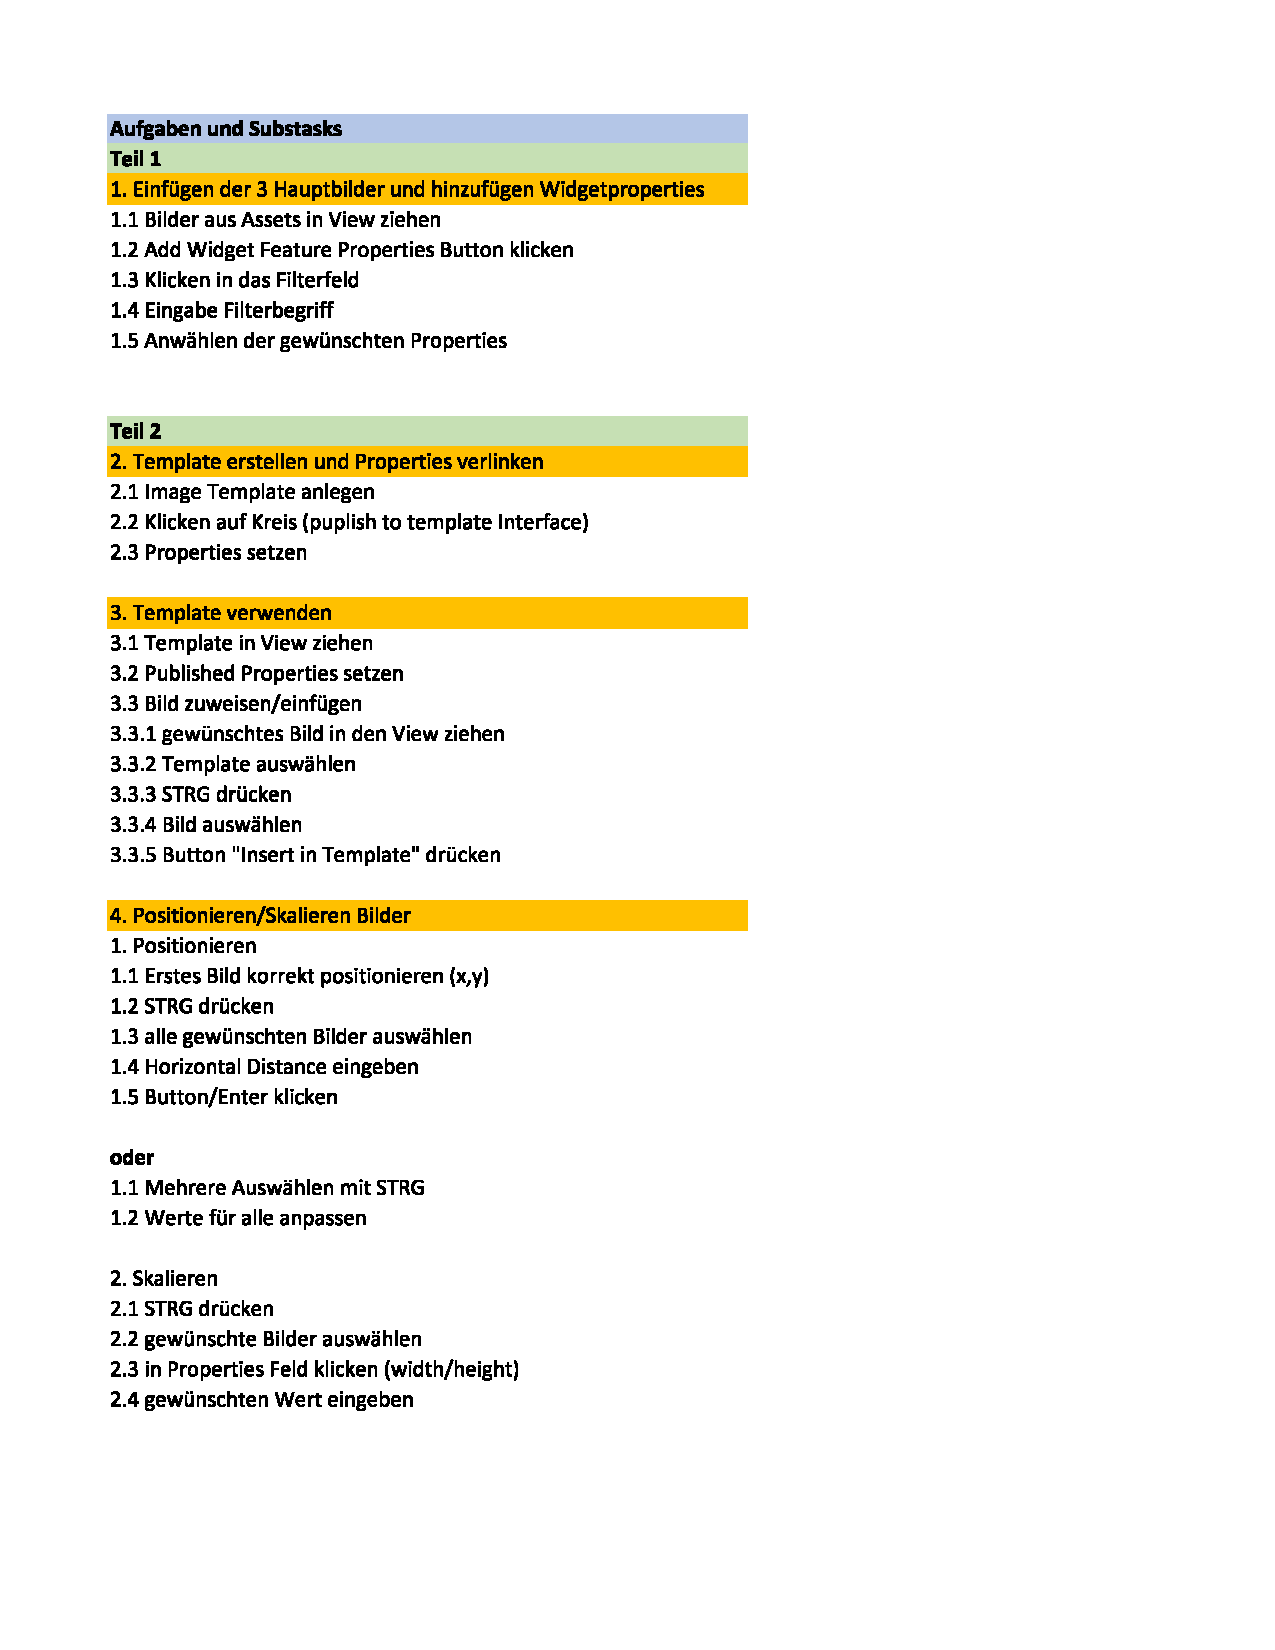
\includegraphics[scale=0.9]{supplement/Subtasks_01.pdf}
\end{center}

\begin{center}
  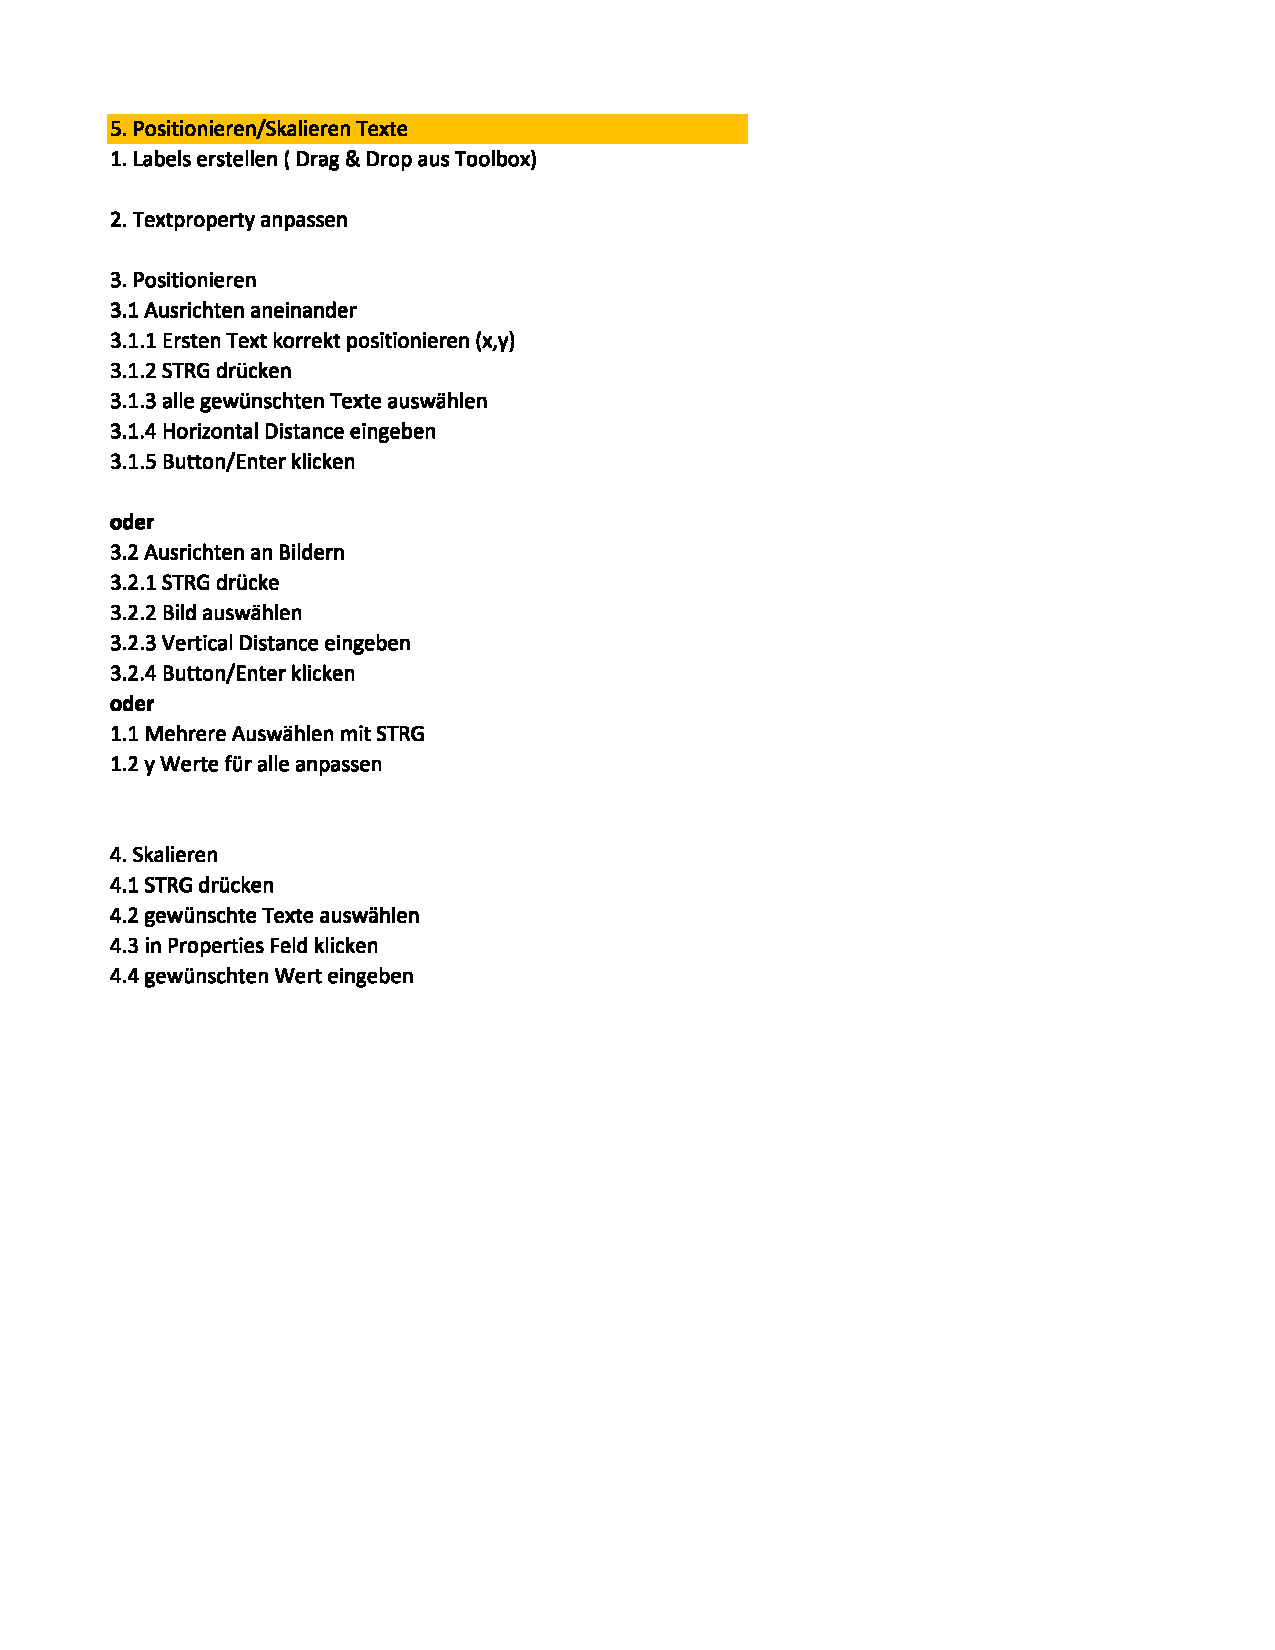
\includegraphics[scale=0.9]{supplement/Subtasks_02.pdf}
\end{center}

\chapter{Arbeitsaufgabe Implementierter Filter}\label{app:Aufgabe_Filter}
\begin{center}
  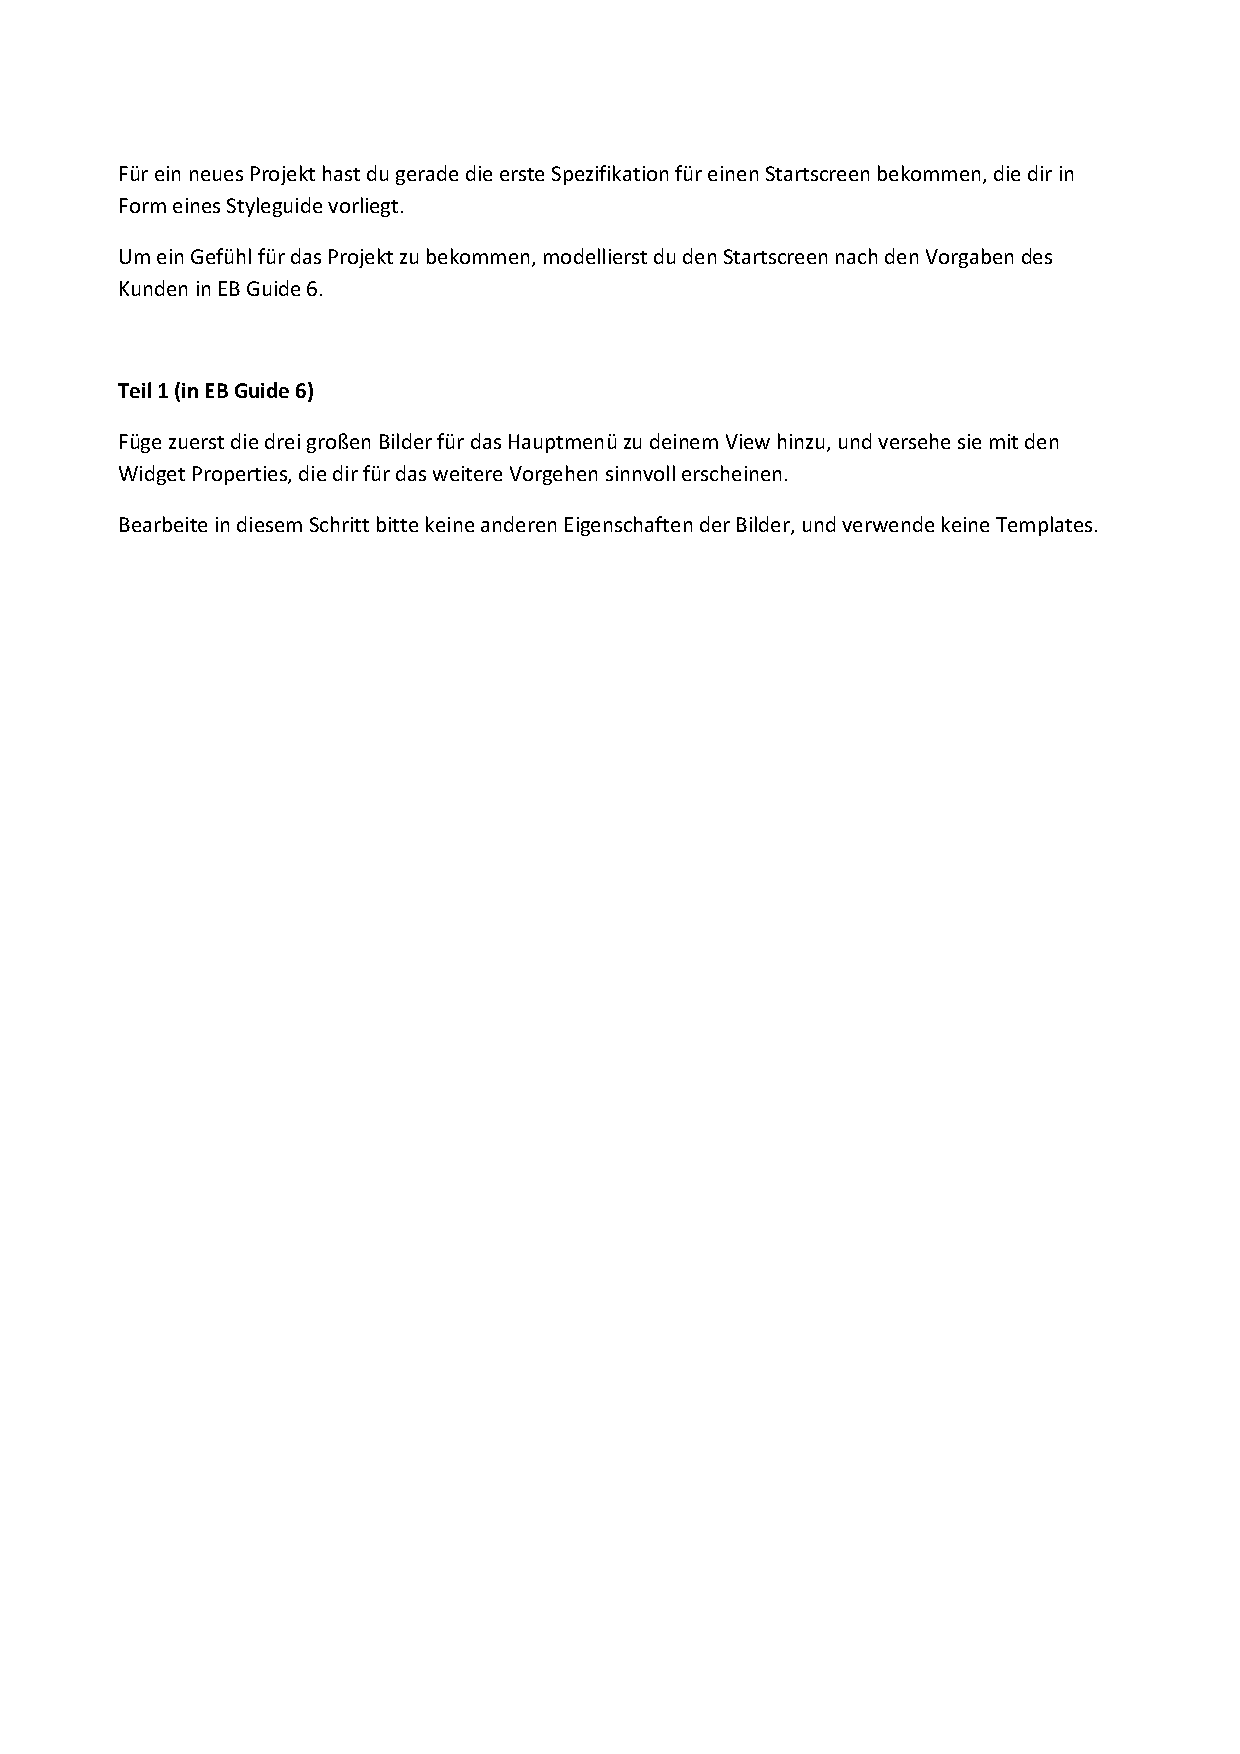
\includegraphics[scale=0.9]{supplement/Arbeitsaufgabe_Prototyp_Teil1.pdf}
\end{center}

\chapter{Arbeitsaufgabe Prototyp}\label{app:Aufgabe_Prototyp}
\begin{center}
  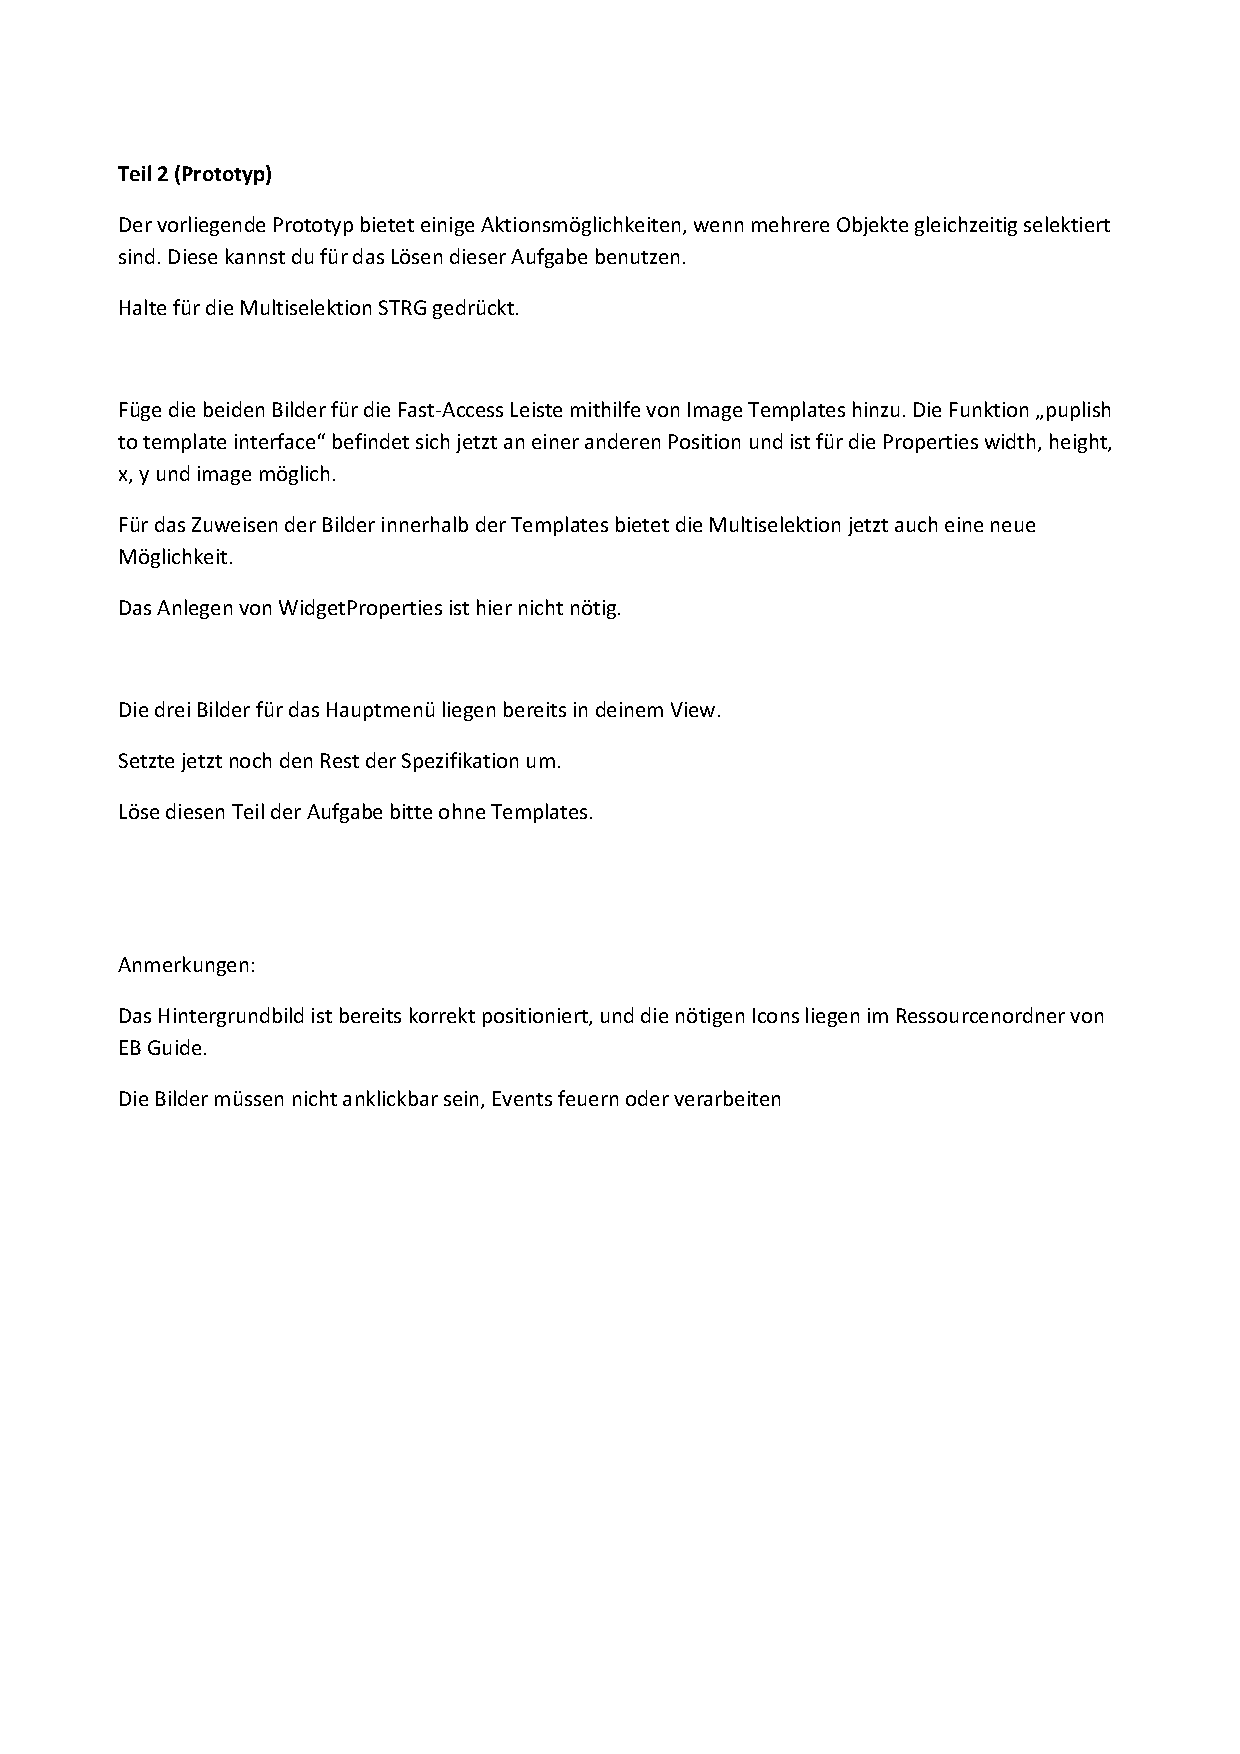
\includegraphics[scale=0.9]{supplement/Arbeitsaufgabe_Prototyp_Teil2.pdf}
\end{center}

\chapter{Arbeitsaufgabe bestehende Software}\label{app:Aufgabe_Guide}
\begin{center}
  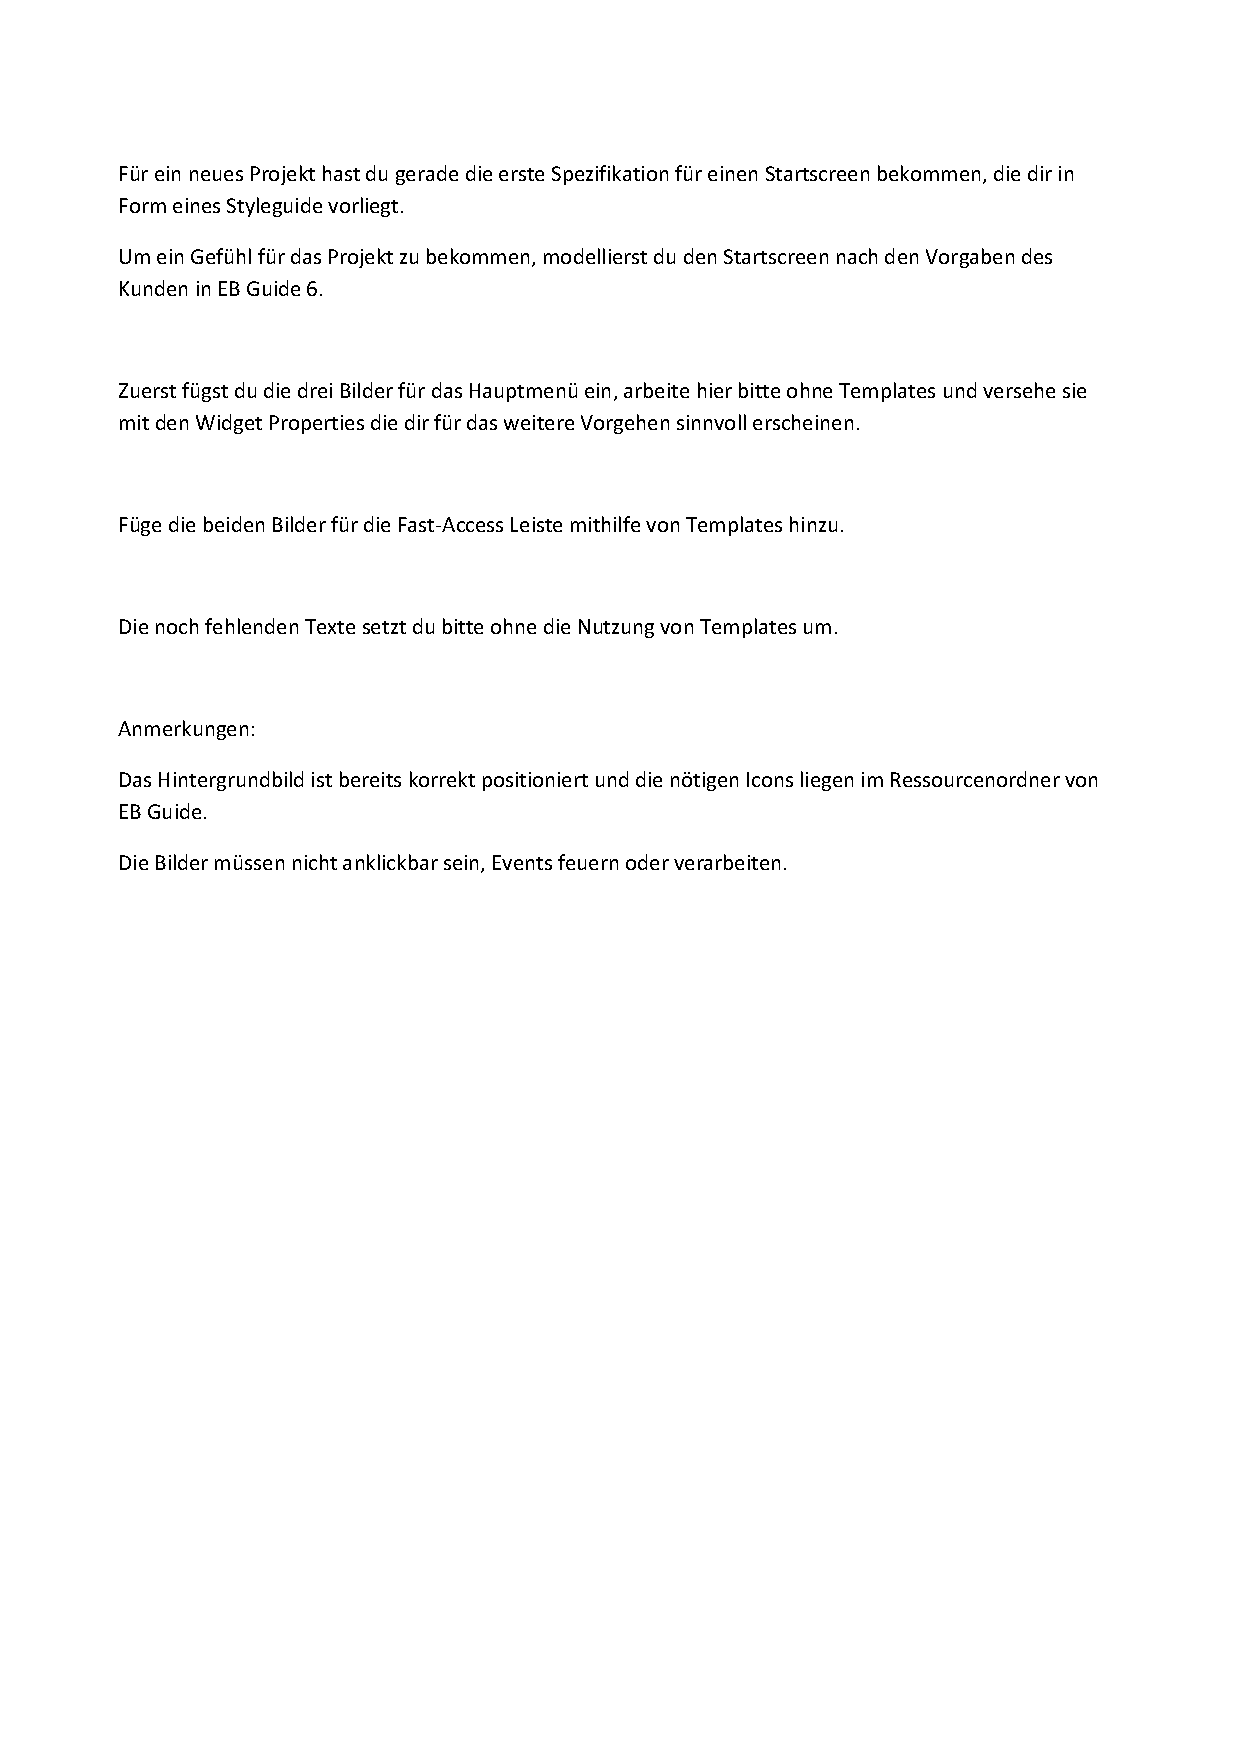
\includegraphics[scale=0.9]{supplement/Arbeitsaufgabe_Guide.pdf}
\end{center}



\backmatter
\listoffigures
\cleardoublepage

\listoftables
\cleardoublepage

\renewcommand{\lstlistlistingname}{Liste der Auflistungen}  % change for German thesis
\lstlistoflistings
\cleardoublepage

\bibliographystyle{wmaainf}
\bibliography{refs}

\end{document}
